%*******************************************************************************
%****************************** Sixth Chapter *********************************
%*******************************************************************************

\chapter{Analysis of LISP mobility and ns-3 implementation}
\label{cha:ns-3}

% **************************** Define Graphics Path **************************
\ifpdf
    \graphicspath{{Chapter7/Pics/Raster/}{Chapter7/Pics/PDF/}{Chapter7/}}
\else
    \graphicspath{{Chapter7/Pics/Vector/}{Chapter7/}}
\fi

%-< ABSTRACT >--------------------------------------------------------------------
The \emph{Locator/Identifier Separation Protocol} (LISP) reconstructing the current IP addressing space brings the benefits to the mobility. LISP Mobile Node (LISP-MN) is based on the basic LISP functionality to provide mobility across networks. Thus, LISP can be implemented either on the border routers or directly on the end hosts to manage mobility. However, there are no experimental results comparing the advantages and disadvantages of each solution. Assessing the LISP mobility performance needs the testbeds or the simulators. The basic LISP architecture is deployed on LISP Beta Network and LISP-Lab platform to offer the researchers a realistic experimental environment, but both do not support LISP-MN. Moreover, since the simulators can help researchers quickly verify the proposals and test new features, we plan to implement a LISP simulator with the mobility extensions.
% Some simulation models with LISP extensions are implemented on various simulators, but are not open source. Fortunately, there is an open source project implementing the fundamental LISP on ns-3 in 2016. Providing a free and flexible LISP simulator so to help researchers quickly test new LISP mobility behaviors motivates our work. 
This chapter introduces the implementation of LISP mobility extensions under ns-3.27 leveraging on an open source basic LISP simulator. In addition, this chapter analyzes the different LISP mobility scenarios from the respects of handover delay and overhead of LISP Control Plane. It describes the characteristics of each scenario. % It also provides the evaluation results in mobility scenario to validate the model and shows when the current proposal of LISP-MN is behind a LISP-site has a very high delay during the handover procedure.

The rest of chapter is organized as follows: Sec.~\ref{sec:ns3_ns3} and Sec.~\ref{sec:ns3_basic_lisp} respectively introduces ns-3 and the existing LISP simulator on it. Sec.~\ref{sec:ns3_lispmn} analyzes the design and implementation of our prototype, and afterwards, Sec.~\ref{sec:ns3_analysis} illustrates three different LISP scenarios supporting mobility, presents their traffic schema, modelizes the handover delay and overhead of LISP Control Plane, and compares their advantages and disadvantages. % Sec.~\ref{sec:evaluation} presents preliminary evaluation results of our implementations. 
Sec.~\ref{sec:ns3_conclusion} provides some ideas of evaluation based on the proposed simulation for future work.
%-< ABSTRACT >--------------------------------------------------------------------

%%-< SECTION >--------------------------------------------------------------------
%\section{Related work}
%\label{sec:ns3_related_work}
\section{NS-3}
\label{sec:ns3_ns3}
ns-3~\cite{ns3} is a popular and free discrete-event network simulator for networking research. It is developed completely in the C++ programming language. %, because it better facilitated the inclusion of C-based implementation code. 
The ns-3 architecture is similar to Linux computers with application, TCP/IP protocol stack, network interface, sockets, etc. ns-3 is very well documented and has an active community which facilitate the researches to adapt ns-3 source code for their researches. Besides, ns-3 offers the possibility to visualize the simulation instance so to allow the users to visually confirm the packets flow as they expect. 
%\begin{itemize}
%    \item Description of ns-3.
%    \item The simulator supporting LISP is introduced in Sec.~\ref{subsec:implementation_OMNet}.
%\end{itemize}

%-< SUB SECTION >--------------------------------------------------------------------
\section{Basic LISP implementation on ns-3}
\label{sec:ns3_basic_lisp}
Simulation is becoming more important for deploying new technologies or as a proof of concept of new protocols. In the study of LISP, there exist few simulators based on OMNet++~\cite{vesely2015locator, vesely2014multicast, klein2012integration} or based on Java~\cite{stockmayer2016jlisp}. However, these existing simulators are not open-source, which hinders other researchers to modify or adapt the simulator with respect to their own research purposes.

To our best knowledge, the unique open-source LISP simulator that we found in the literature is the one proposed by Agbodjan~\cite{lionel2016}. The authors implemented a basic LISP simulator under ns-3.24, but this work can be further polished. For example, the encoding of LISP Control Plane messages does not respect RFC 6830~\cite{rfc6830} so that the Wireshark~\cite{wireshark} can not resolve the captured results in the correct format. % and there exist some bugs when using this simulator. 
More importantly, its implementation has no support for LISP mobility. % Our implementation work is inspired by work of~\cite{lionel2016}. 
By leveraging the source code of Agbodjan, we implement an open source LISP simulator with LISP mobility extension. Besides, we also cover the shortage of the original source code. For example, the encoding of LISP control messages is according to RFC 6830~\cite{rfc6830} so that Wireshark can correctly decode these messages for analysis. The case of Negative Map-Reply has been covered. Recall that the work of Agbodjan is still under ns-3.24, but ns-3.24 evolved lots from ns-3 to the latest version ns-3.27. This implementation is under ns-3.27, which allows the other researchers to profit the newest functionalities of ns-3 simulator.

 
%-< SECTION >--------------------------------------------------------------------
\section{ LISP mobility extensions on ns-3}
\label{sec:ns3_lispmn}
Our implementation respects LISP RFC 6830~\cite{rfc6830} and LISP mobility standards~\cite{meyer2016lisp}. As a design choice, we implement LISP and LISP mobility functionalities by modifying and extending two already existing modules of ns-3:~\emph{internet} and \emph{internet-apps}, instead of by creating a new independent module. The justification behind this design is that LISP protocol and legacy Internet module have an interdependent relationship: an IP layer packet is processed by LISP and then passed to IP protocol again. However, this kind mutually dependent relationship between modules is not supported by ns-3. Our implementation consists of two parts: LISP Data Plane and LISP Control Plane. The communication between LISP Data and Control Plane is achieved via a dedicated socket (i.e. \emph{LispMappingSocket}) that inherits from ns-3 \emph{Socket} class. The Data Plane implementation is in "kernel space" (i.e. ns-3's \emph{TCP/IP stack}) and Control Plane is implemented in "user space" (i.e. ns-3 \emph{Application}). Such a design is inspired by that of OpenLISP~\cite{saucez2009openlisp}.  

The UML diagram of proposed LISP and LISP mobility implementation is illustrated Fig.~\ref{LISP_UML}. The darker blocks are classes already in ns-3, while the white blocks refer to the classes that Agbodjan~\cite{lionel2016} added into ns-3. It should be noted that our implementation keeps the same class names used in the Agbodjan's implementation. Except for the class~\emph{Header}, we rewrite the contents of all his classes to support LISP mobility, especially for the  class~\emph{LispEtrItrApplication},~\emph{LispOverIpv4Impl}, and~\emph{BasicMapTables}. % \yue{Add one sentence to differentiate our work compared with Lionel's work.} 
This work currently only supports IPv4 at time of this writing. The IPv6 support (i.e. the implementation related to IPv6 such as \emph{LispOverIpv6Impl}) is still in process. In addition, the authentication procedure involved in LISP is not considered in our implementation.% \yue{This figure should be revised. For example, LispHeader should be renamed as LispDataPlaneHeader. MapTable should contains a list of MapEntry.}
%-< FIGURE >--------------------------------------------------------------------
\begin{figure*}[!t]
	\centering
	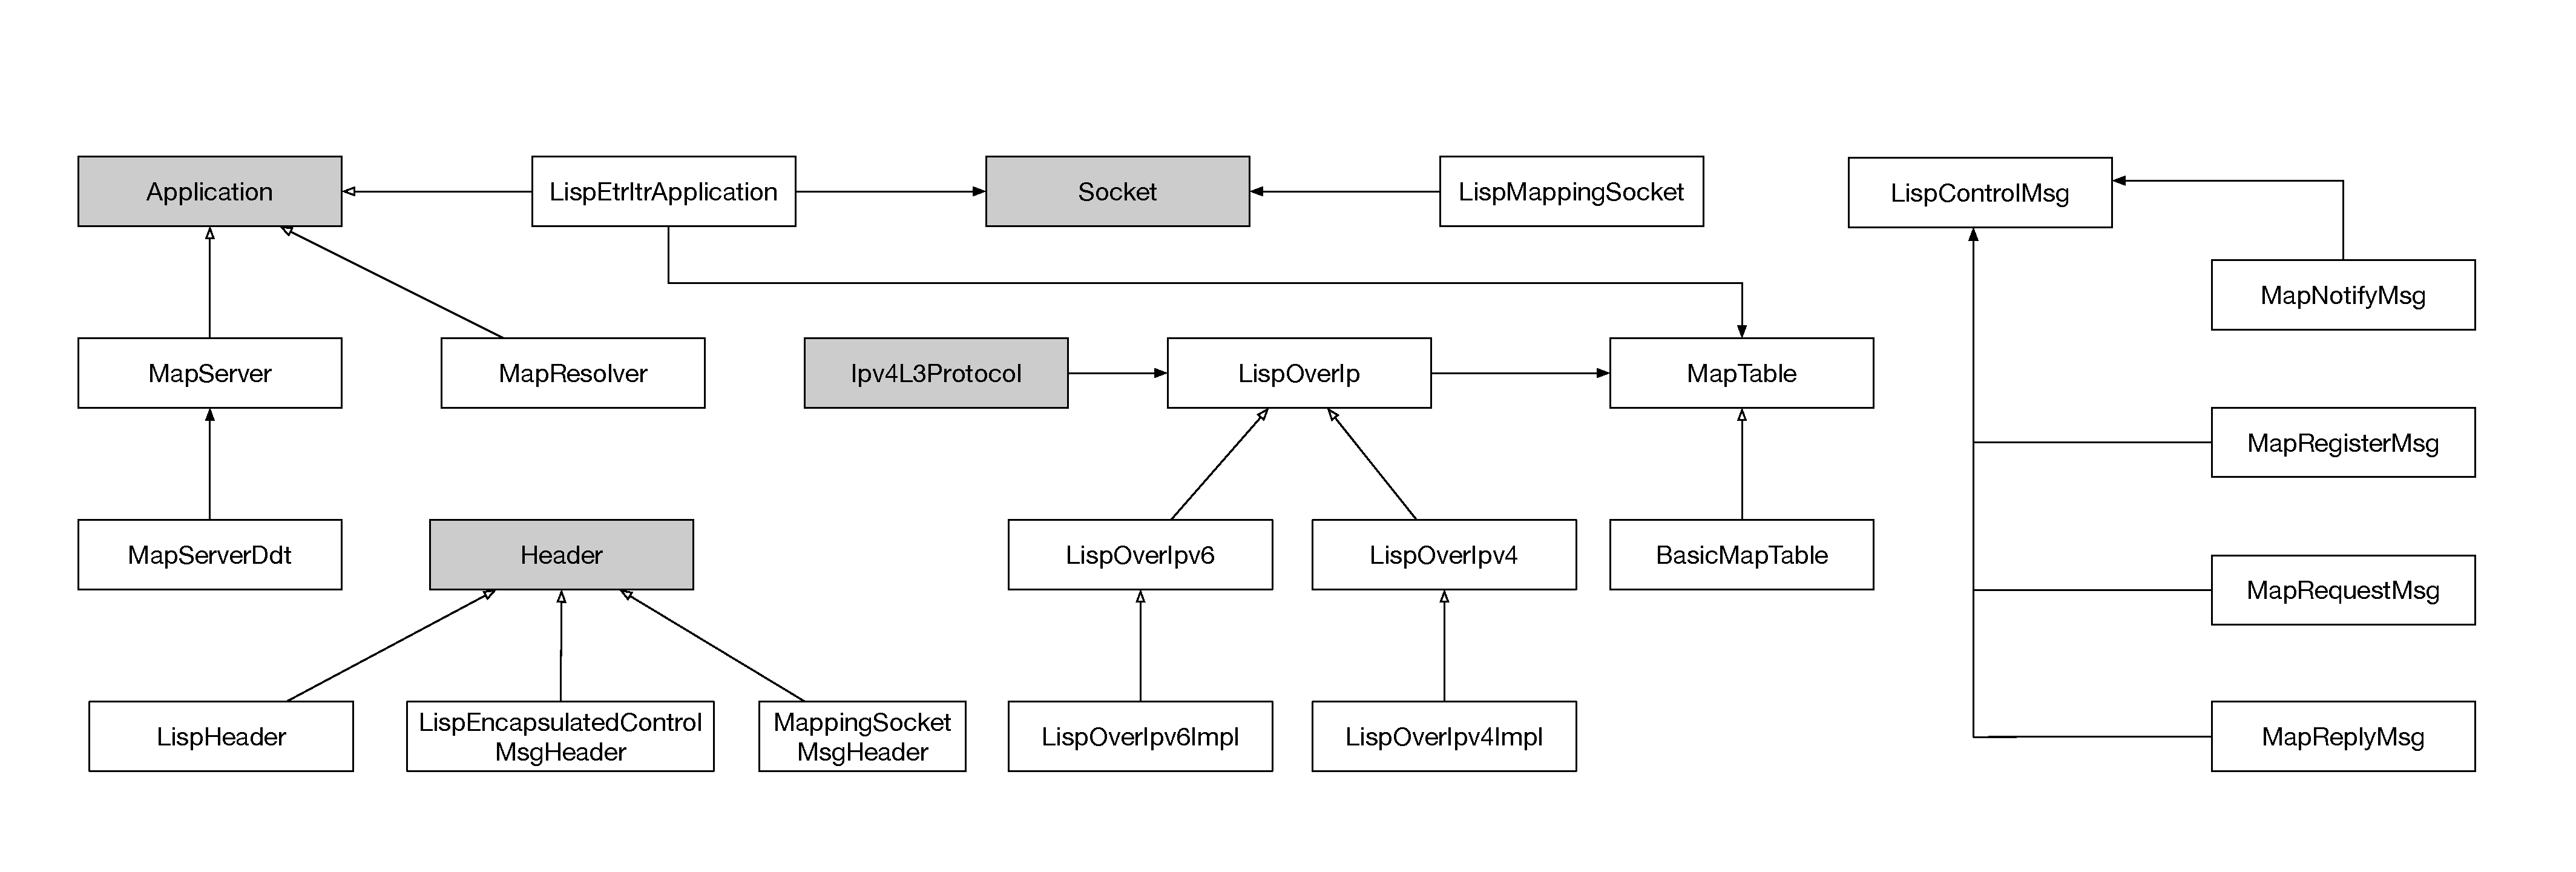
\includegraphics[width=\textwidth]{Pics/LISP_NS3_UML}
	\caption{UML diagram of LISP and LISP mobility implementation. The solid arrow refers to a composition relation, while the blank one refers to a inheritance relation.}
	\label{LISP_UML}
\end{figure*}
%-< END FIGURE >--------------------------------------------------------------------
%-< SUB SECTION >--------------------------------------------------------------------
\subsection{Implementation of LISP Data Plane}
\label{subsec:modifyInternet}
%\begin{itemize}
%    \item Modification of Receive method
%    \item Modification of Delivery method
%    \item Implementation of LISP encapsulation and decapsulation
%\end{itemize}
The implementation of LISP Data Plane mainly consists of \emph{LispOverIp} and \emph{MapTable} classes and their subclasses, along side with some auxiliary classes (e.g. \emph{LispHeader}). In addition, to support LISP functionalites, \emph{Ipv4L3Protcol}'s packet transmission, reception, forward and delivery procedures are accordingly adapted.
\subsubsection{LISP database and cache}
\label{subsec:database-impl}
Each LISP-speaking node should maintain one LISP database and LISP cache for LISP encapsulation and decapsulation operations. In our implementation, both LISP database and cache are modellized by the same class~\emph{MapTable} that stores and manages EID-RLOC mapping information. This class is in charge of CRUD (Create, Retrieve, Update, Delete) operations for mappings. Each mapping entry in LISP database and cache is an instance of \emph{MapEntry}. For the sake of flexibility, the class \emph{MapTable} is an abstract base class. The CRUD methods are implemented in its subclass \emph{BasicMapTable}. The mapping search operation is a straightforward iteration over LISP database or cache. It is possible that for other users to provide their own LISP database and cache implementation, for example, which uses more sophisticated mapping entry look up algorithms, by extending \emph{MapTable} class.

In addition, \emph{MapTable} has a callback which allows to send the buffered packet (either LISP Data Plane or Control Plane) %\yue{Recall that now I add a callback into MapTable and I only implement the resending once the required cache is inserted into cache. WE currently only use this for LISP-control messages (SMR-invoked Map Request). We can easily extend this to support other LISP data plane packets buffering and resending once the required EID-RLOC mapping is obtained.} 
due to LISP cache miss event, upon insertion of the required EID-RLOC mapping information into LISP cache.

\subsubsection{Implementation of LISP encapsulation and decapsulation}
To integrate LISP and LISP mobility into conventional Internet protocol stack, one key technical difficulty is that \emph{Ipv4L3Protcol} should be able to determine when passing a packet being processed to LISP-related procedure and how to retrieve the associated mapping information. To this end, a new class called \emph{LispOverIp} and its extended classes 
%(refer to Fig.~\ref{LISP_UML}) 
are added to ns-3 \emph{internet} module. This class is in charge of checking whether it is necessary to do LISP-related operations (\emph{NeedEncapsulation()}, \emph{NeedDecapsulation()}), and encapsulating conventional IP packets (i.e., \emph{LispOutput()}) as well as decapsulating LISP packets(\emph{LispInput()}). It contains a smart pointer\footnote{A smart pointer is an abstract data type introduced in C++ that simulates a pointer while providing additional features, such as automatic memory management or bounds checking.} pointing to the LISP database and LISP cache (e.g.~\emph{MapTable}) on which executes mapping search.
%\begin{figure*}[!t]
%	\centering
%	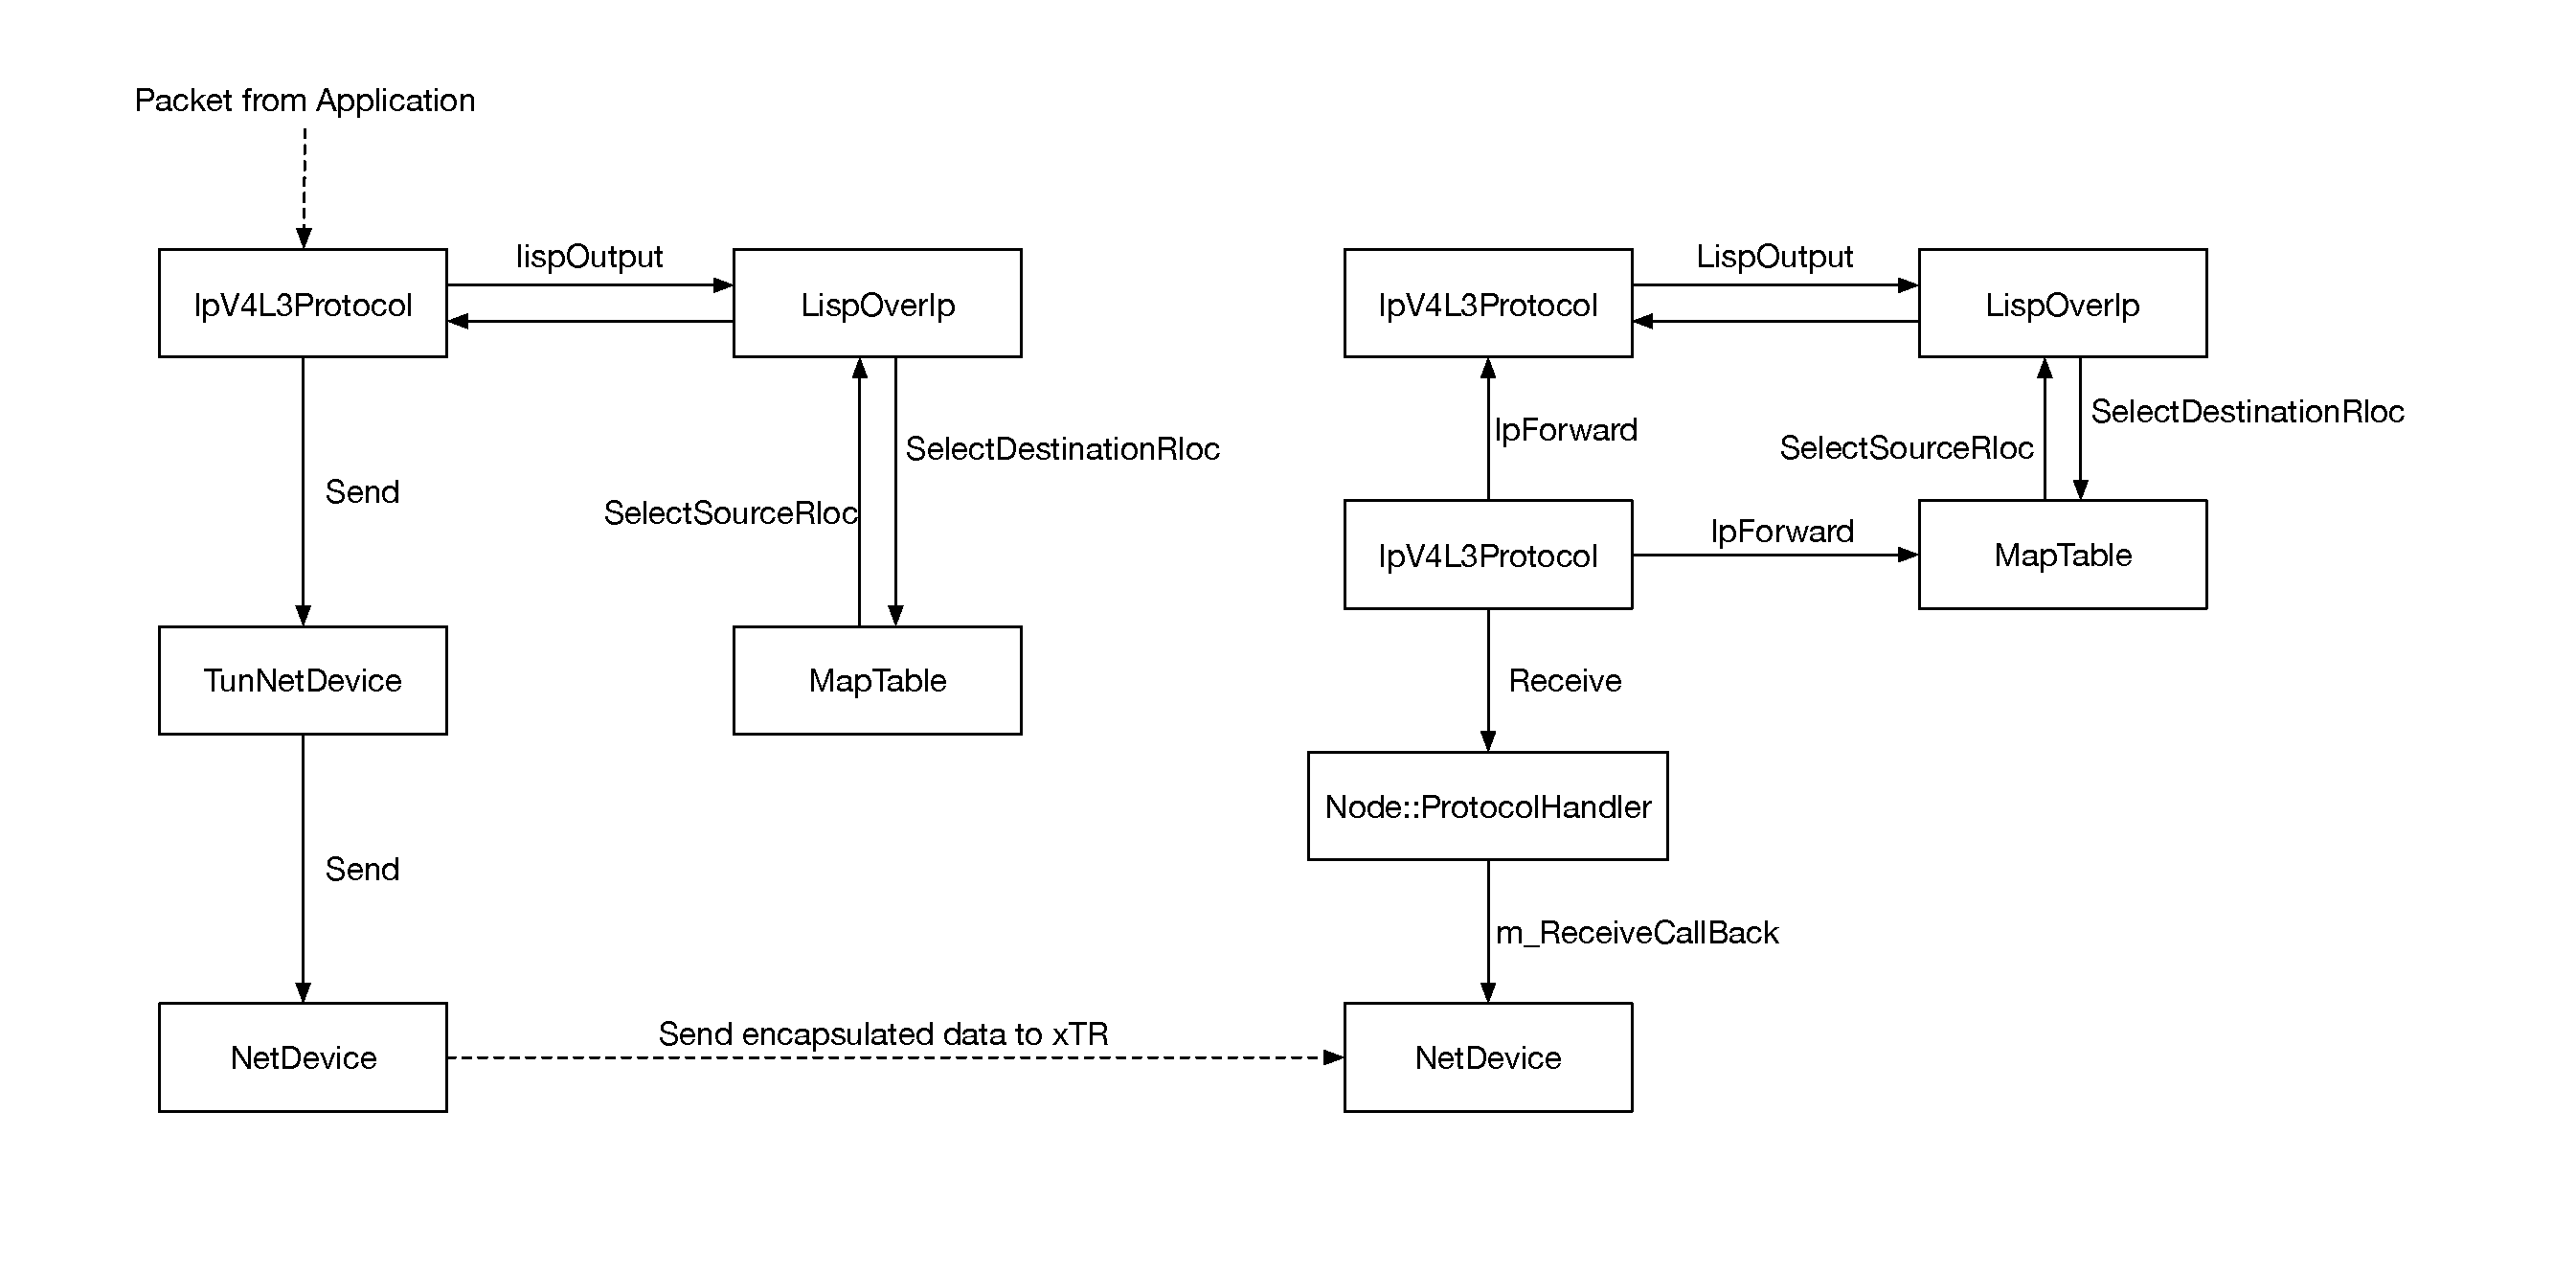
\includegraphics[width=\textwidth]{Pics/ns3_lisp_data_plane.eps}
%	\caption{Illustration of LISP encapsulation and decapsulation} 
%%	\yue{This figure is actually the process of MN, xTR1/2. I forgot to draw to the processing of xTR3 and CN. I will make a draft of the left part and send it to you as soon as possible.}
%	\label{fig:ns3-lisp-data-plane}
%\end{figure*}

We take the double encapsulation example shown in Fig.~\ref{LISP_archi_2encap} to illustrate how LISP encapsulation and decapsulation is implemented. We assume that the required mapping entries during LISP Data Plane operations are already in LISP-MN cache. A LISP-speaking node behind the $xTR_1$ needs to communicate with CN behind the $xTR_3$. Thus, a packet should be encapsulated within the considered node and forwarded to the $xTR_1$. Subsequently, the packet is further encapsulated and forwarded. At the $xTR_3$, % xTR which serves the CN, 
the received packet is decapsulated twice and forwarded. Thus, the example involves packet transmission, forwarding and reception 
%is illustrated in Fig.~\ref{fig:ns3-lisp-data-plane}. 

Within the LISP-MN node, when the upper layer of IP protocol calls the \emph{Send()} method of \emph{Ipv4L3Protcol}, a packet comes down to IP layer. The \emph{Send()} method is adapted so that it first verifies whether the \emph{LispOverIp} object is present. If yes, some checks are then conducted to determine that this packet should be processed by \emph{LispOutput()} (to encapsulate the packets) or by conventional packet transmission routine. For example, if both source and destination IP address of this packet belong to the same network, the LISP-related process (e.g., encapsulation) is skipped and this packet is processed as in a non-LISP network. Otherwise, EID-RLOC mapping information is searched from LISP cache and LISP database on LISP-MN node. 

After encapsulation and forwarding, the considered packet is forwarded to $xTR_1$. % This procedure is also illustrated in Fig.~\ref{fig:ns3-lisp-data-plane}. 
Low layer invokes the \emph{Receive()} method of \emph{Ipv4L3Protocol} to pass this packet to IP layer. Since this packet is destinated to a remote CN instead of itself, this packet is processed by patched \emph{IpForward()} method. % , \emph{IpForward} method of \emph{Ipv4L3Protocol} is called. 
With this method, LISP encapsulation is verified. \emph{LispOverIp} looks for the source RLOC (RLOC of $xTR_1$) and destination RLOC (RLOC of $xTR_3$) for the outer IP header building. Once this step is done, \emph{Ipv4L3Protocol}'s \emph{Send()} method transmits these encapsulated packet to MAC layer for transmission.

When this packet arrives at $xTR_3$ which servers CN, $xTR_3$ finds that the destination of this packet is the node itself, the packet is processed by \emph{LocalDelivery()} method in \emph{Ipv4L3Protocol}. Before passing to transport layer, \emph{LocalDelivery} checks if the packet should be decapsulated. If yes, it is passed to \emph{LispInput()} method, in which the packet is decapsulated and re-injected into the IP stack. That is to say, \emph{Receive()} method is called again after decapsulation operation. If the packet still has LISP header, the aforementioned procedure will repeated until it has no need to be decapsulated. Finally, the packet with source address of LISP-MN and destination address of CN is forwarded to CN.

%-< SUB SECTION >--------------------------------------------------------------------
\subsection{Implementation of LISP Control Plane}
\label{subsec:control-plane-impl}
%\begin{itemize}
%    \item Implementation of xTR under ns3
%    \item Implementation of MS under ns3
%    \item Socket communication between control plan and data plan
%\end{itemize}
The implementation of LISP Control Plane at least should provide ITR/ETR, MR and MS. In practice, ITR and ETR functionalities are usually placed on a same router called xTR. In our implementation, they are included into class \emph{LispEtrItrApplication}. The functionalities of MR and MS are respectively implemented by class \emph{MapResolver} and \emph{MapServer}. The LISP Control Plane messages (Map-Register, Map-Request, etc.) are represented by the derived classes of \emph{LispControlMsg}. In addition, to communicate with LISP Data Plane, a socket class \emph{LispMappingSocket} is proposed.

\subsubsection{Implementation of xTR functionalities}
A ns-3 node that runs \emph{LispEtrItrApplication} is a LISP-compatible router. It should be able to communicate with \emph{LispOverIp} on the same node (e.g. inform cache missing event) and other LISP-compatible routers (e.g. Map-Request/Map-Reply). 
\begin{figure*}[!t]
	\centering
	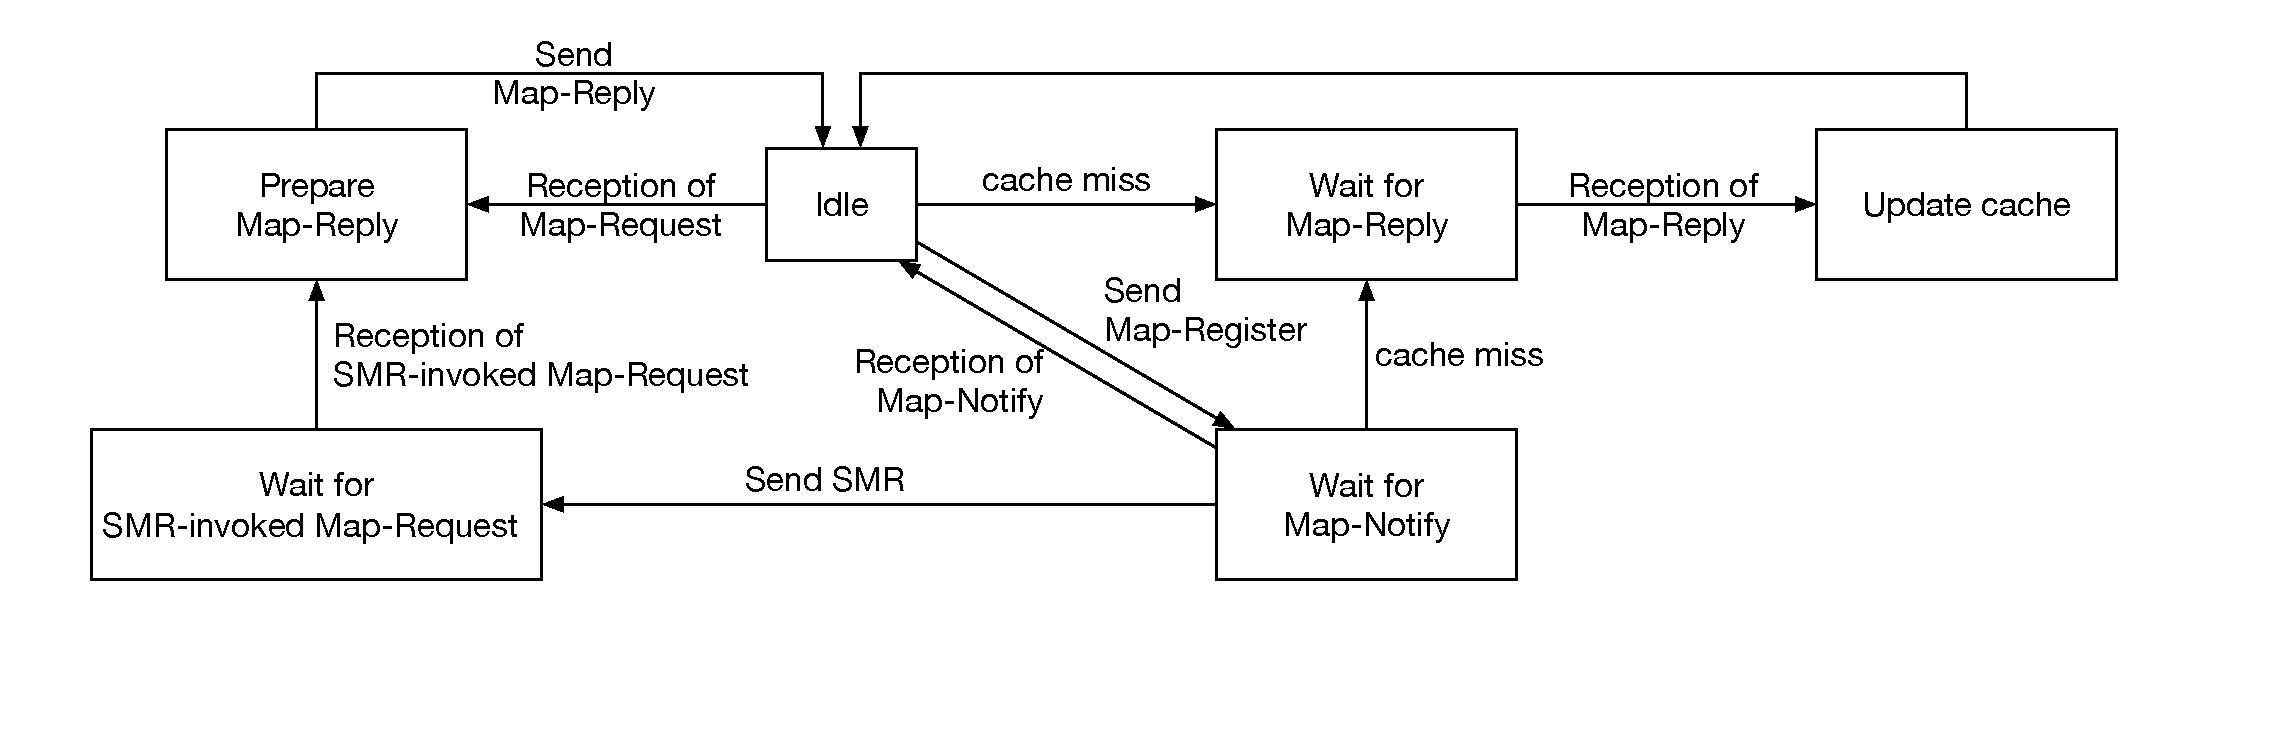
\includegraphics[width=\textwidth]{Pics/xTR_state_transition.eps}
	\caption{State transition diagram of xTR application} % \yue{Good remark. First in a state transition diagram, a block refers to a `state' and an arrow refers to a certain action leading to state change. A state transition diagram identifies all possible states and reflects how a state is transited to another one. Back to this diagram, this state transition diagram is questionable, because this digram reflects the behaviors of the xTR running within LISP-node and the SMR-invoked Map-Request will be sent back to the xTR which previously initiates one SMR. For this scenario, when in state of `Wait for Map-Notify', it has 2 possible actions: if the required EID-RLOC mapping (to xTR2 for example) is known, it can switch to state of `Wait for SMR-invoked' map request by action of 'Send SMR'. Otherwise, a cache miss event occurs and this makes the xTR sends Map-Request message and enter into state of `Wait for Map-Reply'. Conclusion: to be more clear, maybe first change the legend of this figure to "State transition diagram of xTR application running on LISP-MN node. SMR-invoked Map-Request is sent back to the xTR which initiates.". Second, if you think, `cache miss' is misleading. You can change it as `Send Map-Request'. In addition, I think modify the state name `Idle' to `Listening' is better, because xTR is always listening to a UDP port for the incoming LISP control messages. Up to you to make the change. }
	\label{fig:xTR-state-transition}
\end{figure*}
The state transition diagram is illustrated in Fig.~\ref{fig:xTR-state-transition}. When destination RLOC is not found in the cache of xTR (here indicates the xTR functionalities on LISP-MN) for a processed packet, the cache miss event occurs and LISP Data Plane (e.g. \emph{LispOverIp}) notifies \emph{LispEtrItrApplication} on the same LISP-MN node of this event via a \emph{LispMappingSocket} socket. Once reception of cache missing event from LISP Data Plane (i.e. \emph{LispOverIp} object), \emph{LispEtrItrApplication} initiates a Map-Request message to LISP mapping system. Once reception of Map-Reply, the received EID-RLOC mapping is inserted into LISP cache. It should be noted that in our implementation, before the reception of Map-Reply message, all transmitted packets with the required RLOC as desination are dropped. There exists one reception: the processing of SMR-invoked Map-Request message. If the RLOC of xTR initiating the SMR (actually a local RLOC) is not found, SMR-invoked Map-Request message is buffered and sent again once the insertion of required mapping information into LISP cache. This is achievable thanks to a callback associated with LISP cache insert operation.

In case of reception of Map-Request, \emph{LispEtrItrApplication} executes a database look up on \emph{MapTable} and generates the corresponding Map-Reply containing EID-RLOC mapping.

When xTR application starts or LISP database on a node has information update (e.g. during a handover scenario), xTR application sends a Map-Register message and waits for a Map-Notify message. In case of LISP database update, xTR sends a SMR message to all xTR whose RLOC is present in its cache. %, upon the reception of Map-Notify message. 
According to RFC 6830~\cite{rfc6830}, the xTR receiving the SMR has two possibilities of reactions about sending SMR-invoked Map-Request:  towards a mapping system or the xTR initiating this SMR. Both cases are implemented in our work and this can be configured by an attribute of \emph{LispEtrItrApplication}. It should be noted that in double-encapsulation, if SMR-invoked Map-Request is directly sent to LISP-MN node whose LRLOC is unknown for xTR, the first SMR-invoked Map-Request cannot be sent due to cache miss. We implement a callback function within \emph{BasicMapTable} which allows to send immediately the buffered SMR-invoked Map-Request upon insertion of required EID-RLOC mapping into cache. Note that this mechanism is designed only for LISP Control Plane messages. LISP Data Plane is dropped in case of cache miss.

To support LISP-MN feature, \emph{LispEtrItrApplication} also communicates with DHCP client application. For example, once a LISP-MN obtains an IP address from DHCP server, \emph{LispEtrItrApplication} receives the corresponding EID-RLOC mapping and sends a Map-Register message to the Map Server.

\subsubsection{Implementation of MR and MS}
A node that runs a \emph{MapServer} application is the MS in a LISP-supported network. This class has a smart pointer pointing to a LISP database (i.e.~\emph{MapTables}) to store the all EID-RLOC mapping information. This application is always listening to UDP port 4342. Once reception of Map-Register message, it retrieves the EID-RLOC mapping inside, inserts the latter into LISP database and sends a Map-Notify message as response if necessary. %\yue{Because only a certain flag of LISP header is set as 1, a Map-Notify message is sent as a response to Map-Register message. Otherwise, no map-notify is sent. This is defied by RFC 6830.}
Each time MS receives a Map-Request message, it looks up the required EID within its database. If the EID-RLOC mapping is found, map server forwards this request to the corresponding xTR otherwise sends a Negative Map-Reply message to the querying xTR. It is worth to indicating that class \emph{MapServer} is actually an abstract base class. The real functionalities are implemented by its subclasses, which is \emph{MapServerDdt} in our implementation. This design allows the researchers to easily integrate and test their own implementations of MS. In current implementation, the role of MR is to receive the Map-Request message from xTR and forward it to the MS.

\subsection{Modification of DHCP client to support LISP mobility}
\label{subsec:DHCP}
%\begin{itemize}
%    \item LISP-MN, in case of IPv4, need the intervention of DHCP procedure
%    \item The current version of DHCPv4 is not compatible with LISP
%    \item Implementation of LISP-compatible DHCPv4 based on conventional DHCPv4
%\end{itemize}
To support LISP mobility for IPv4, the intervention of DHCP is indispensable. From ns-3.27, DHCP client and server have been implemented in module \emph{internet-apps}. However, the DHCP client of ns-3 is not compatible with LISP. Thus, conventional DHCP client is adapted to support LISP.
\begin{figure*}[!t]
	\centering
	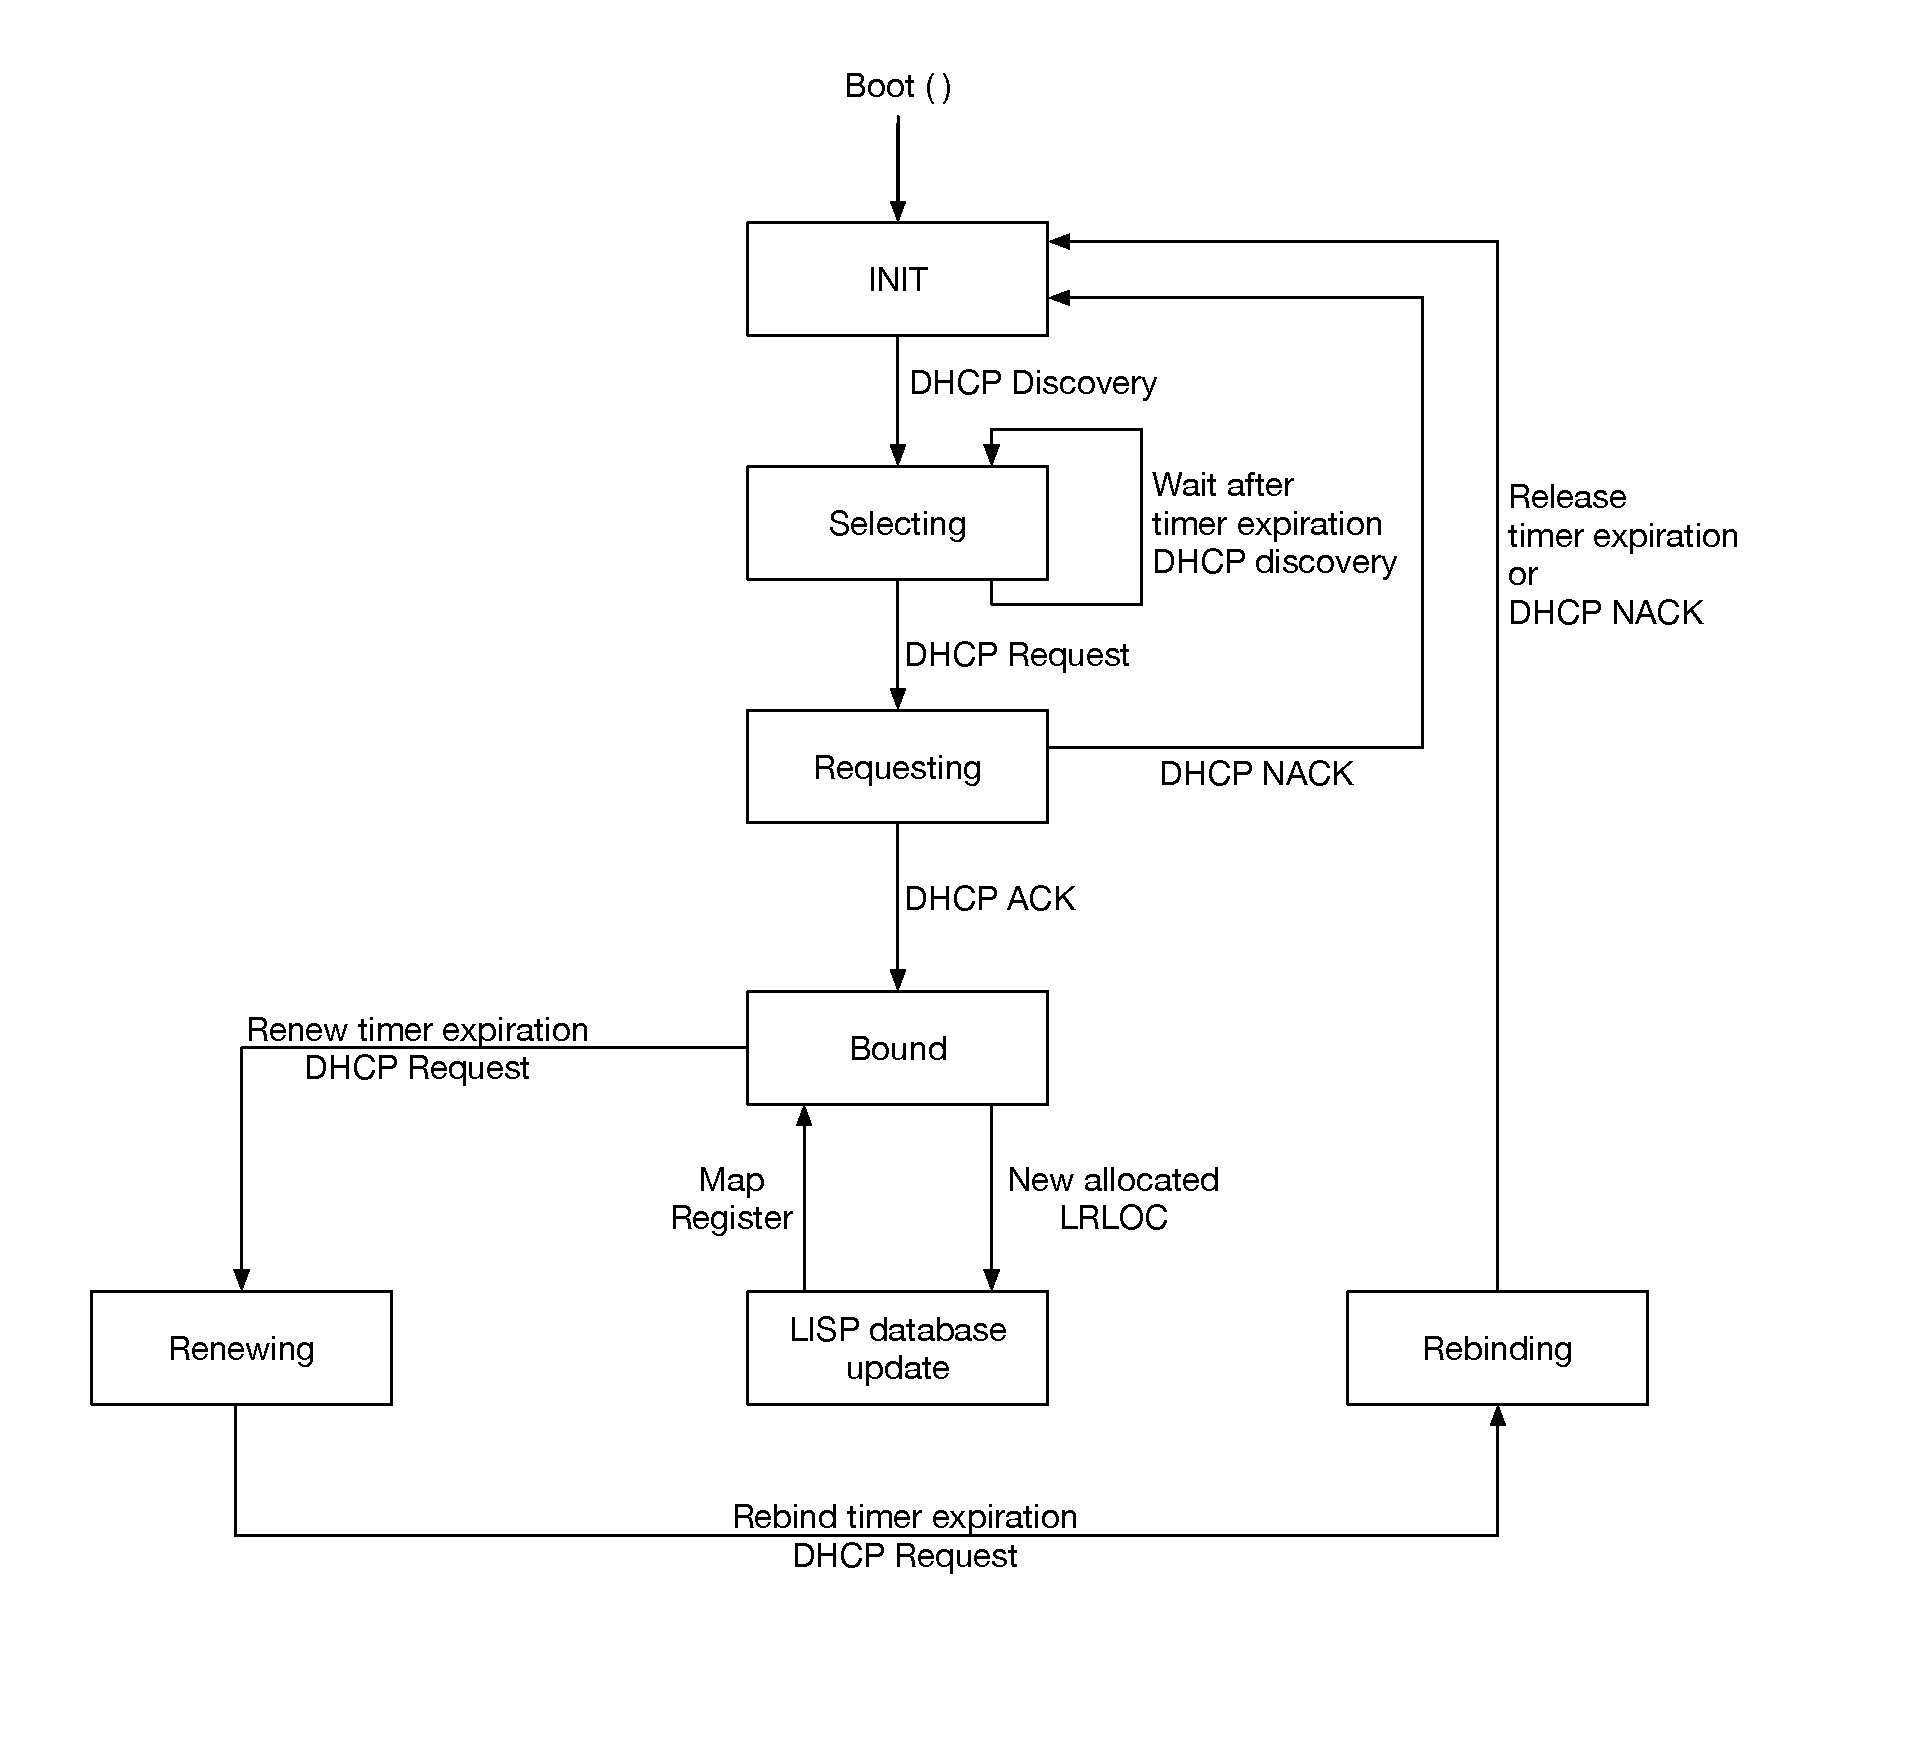
\includegraphics[width=0.9\textwidth]{Pics/DHCP_transition_state.eps}
	\caption{LISP-compatible DHCP client state transition diagram}
	\label{fig:DHCP-state-transition}
\end{figure*}
The state transition diagram of DHCP client is illustrated in Fig.~\ref{fig:DHCP-state-transition}. When a LISP-MN node roams into the area covered by another xTR, the boot procedure of DHCP client is triggered once that the link state is changed. Afterwards, the DHCP client sequentially pass 'INIT', 'Selecting', 'Requesting' states and enter into 'Bound' state after the reception of DHCP ACK message from DHCP server. In 'Bound' state, apart from saving the newly obtained IPv4 address (namely LRLOC) and default gateway, DHCP client should be able to check if the LRLOC is different from the one associated with its EID in its LISP database. If LRLOC is changed, DHCP client enters into state of 'LISP database update'. DHCP client is equipped with a dedicated socket of type \emph{LispMappingSocket}. By this socket, DHCP client notifies the \emph{LispEtrItrApplication} by sending a dedicated message that contains the EID-LRLOC mapping. \emph{LispEtrItrApplication} is in charge of populating the received mapping entry into LISP database and sending a Map-Register message to the Map Server.

To be compatible with DHCP, conventional LISP-related process is also modified. For example, to transmit a DHCP Discovery message (application layer message), its source IP address is set as $0.0.0.0$. The \emph{Send()} method of \emph{Ipv4L3Protocol} should be modified so that this message is not processed \emph{LispOverIp}.

%-< SUB SECTION >--------------------------------------------------------------------
\subsection{Integration of TUN net interface card}
\label{subsec:tundevice}
To support mobility, a LISP-speaking node actually can be regarded as a small LISP-Site. The xTR functionalities and DHCP service should be implemented on the LISP-speaking node. The address of MR and MS should be configured. As a LISP-MN, it has a static permanent EID and dynamic RLOC assigned by the DHCP server. To differentiate with conventional RLOC of xTR interface, such kind of RLOC is referred to as the local RLOC (LRLOC). 
%There exist several possibilities about on which \acrlong{nic}s (\acrshort{nic}s) EID is configured: IP aliasing, loop back device and TUN device. IP aliasing consists of associating more than one IP address to a network interface. In case of LISP mobility, the supplementary IP address is EID. Loop back device can be also configured with EID to support LISP encapsulation. 
As a design choice, we use the solution based on TUN device, which is also applied by Lispmob~\cite{LISPmob}. In our implementation, different from a conventional LISP node, at least two \acrshort{nic}s should be installed into the node. One is normal \acrshort{nic} such as~\emph{WifiNetDevice}. The DHCP client application runs on this kind of card and thus the LRLOC is allocated to this card. The other is a TUN type card. The TUN \acrshort{nic} is a virtual card which should actually invoke~\emph{Send()} of another real \acrshort{nic}. The permanent EID is assigned to TUN device. 

Recall that after DHCP procedure, the node will be configured a default gateway provided by DHCP server. Routing table of LISP-MN are modified so that the packets from application layer always use EID as the source IP address of inner IP header.
%\begin{table}[]
%	\centering
%	\caption{Static route table of LISP-MN}
%	\label{tab:static-route-table}
%	\begin{tabular}{@{}c|c@{}}
%		\hline\hline
%		Destination Prefix & Interface \\ \hline
%		0.0.0.0/1          & TUN       \\ \hline
%		128.0.0.1/1        & TUN      \\  \hline \hline           
%	\end{tabular}
%\end{table}


%-< SUB SECTION >--------------------------------------------------------------------

%-< SECTION >--------------------------------------------------------------------
\section{Theoretical analysis}
\label{sec:ns3_analysis}
IP mobility leveraging on LISP can be implemented either on the border router or the end host. To explore the characteristics of each scheme, we propose the following three different scenarios and analyze the overall handover delay and LISP Control Plane overhead. 
\begin{enumerate}[noitemsep,topsep=0pt]
	\item LISP-MN in the non-LISP-Site (i.e., only the end host supports LISP). 
	\item MN in the LISP-Site (i.e., only the border router supports LISP). 
	\item LISP-MN in the LISP-Site (i.e., both the border router and the end host support LISP). 
\end{enumerate}	
%-< FIGURE >--------------------------------------------------------------------
\begin{figure}[!t]
	\centering
	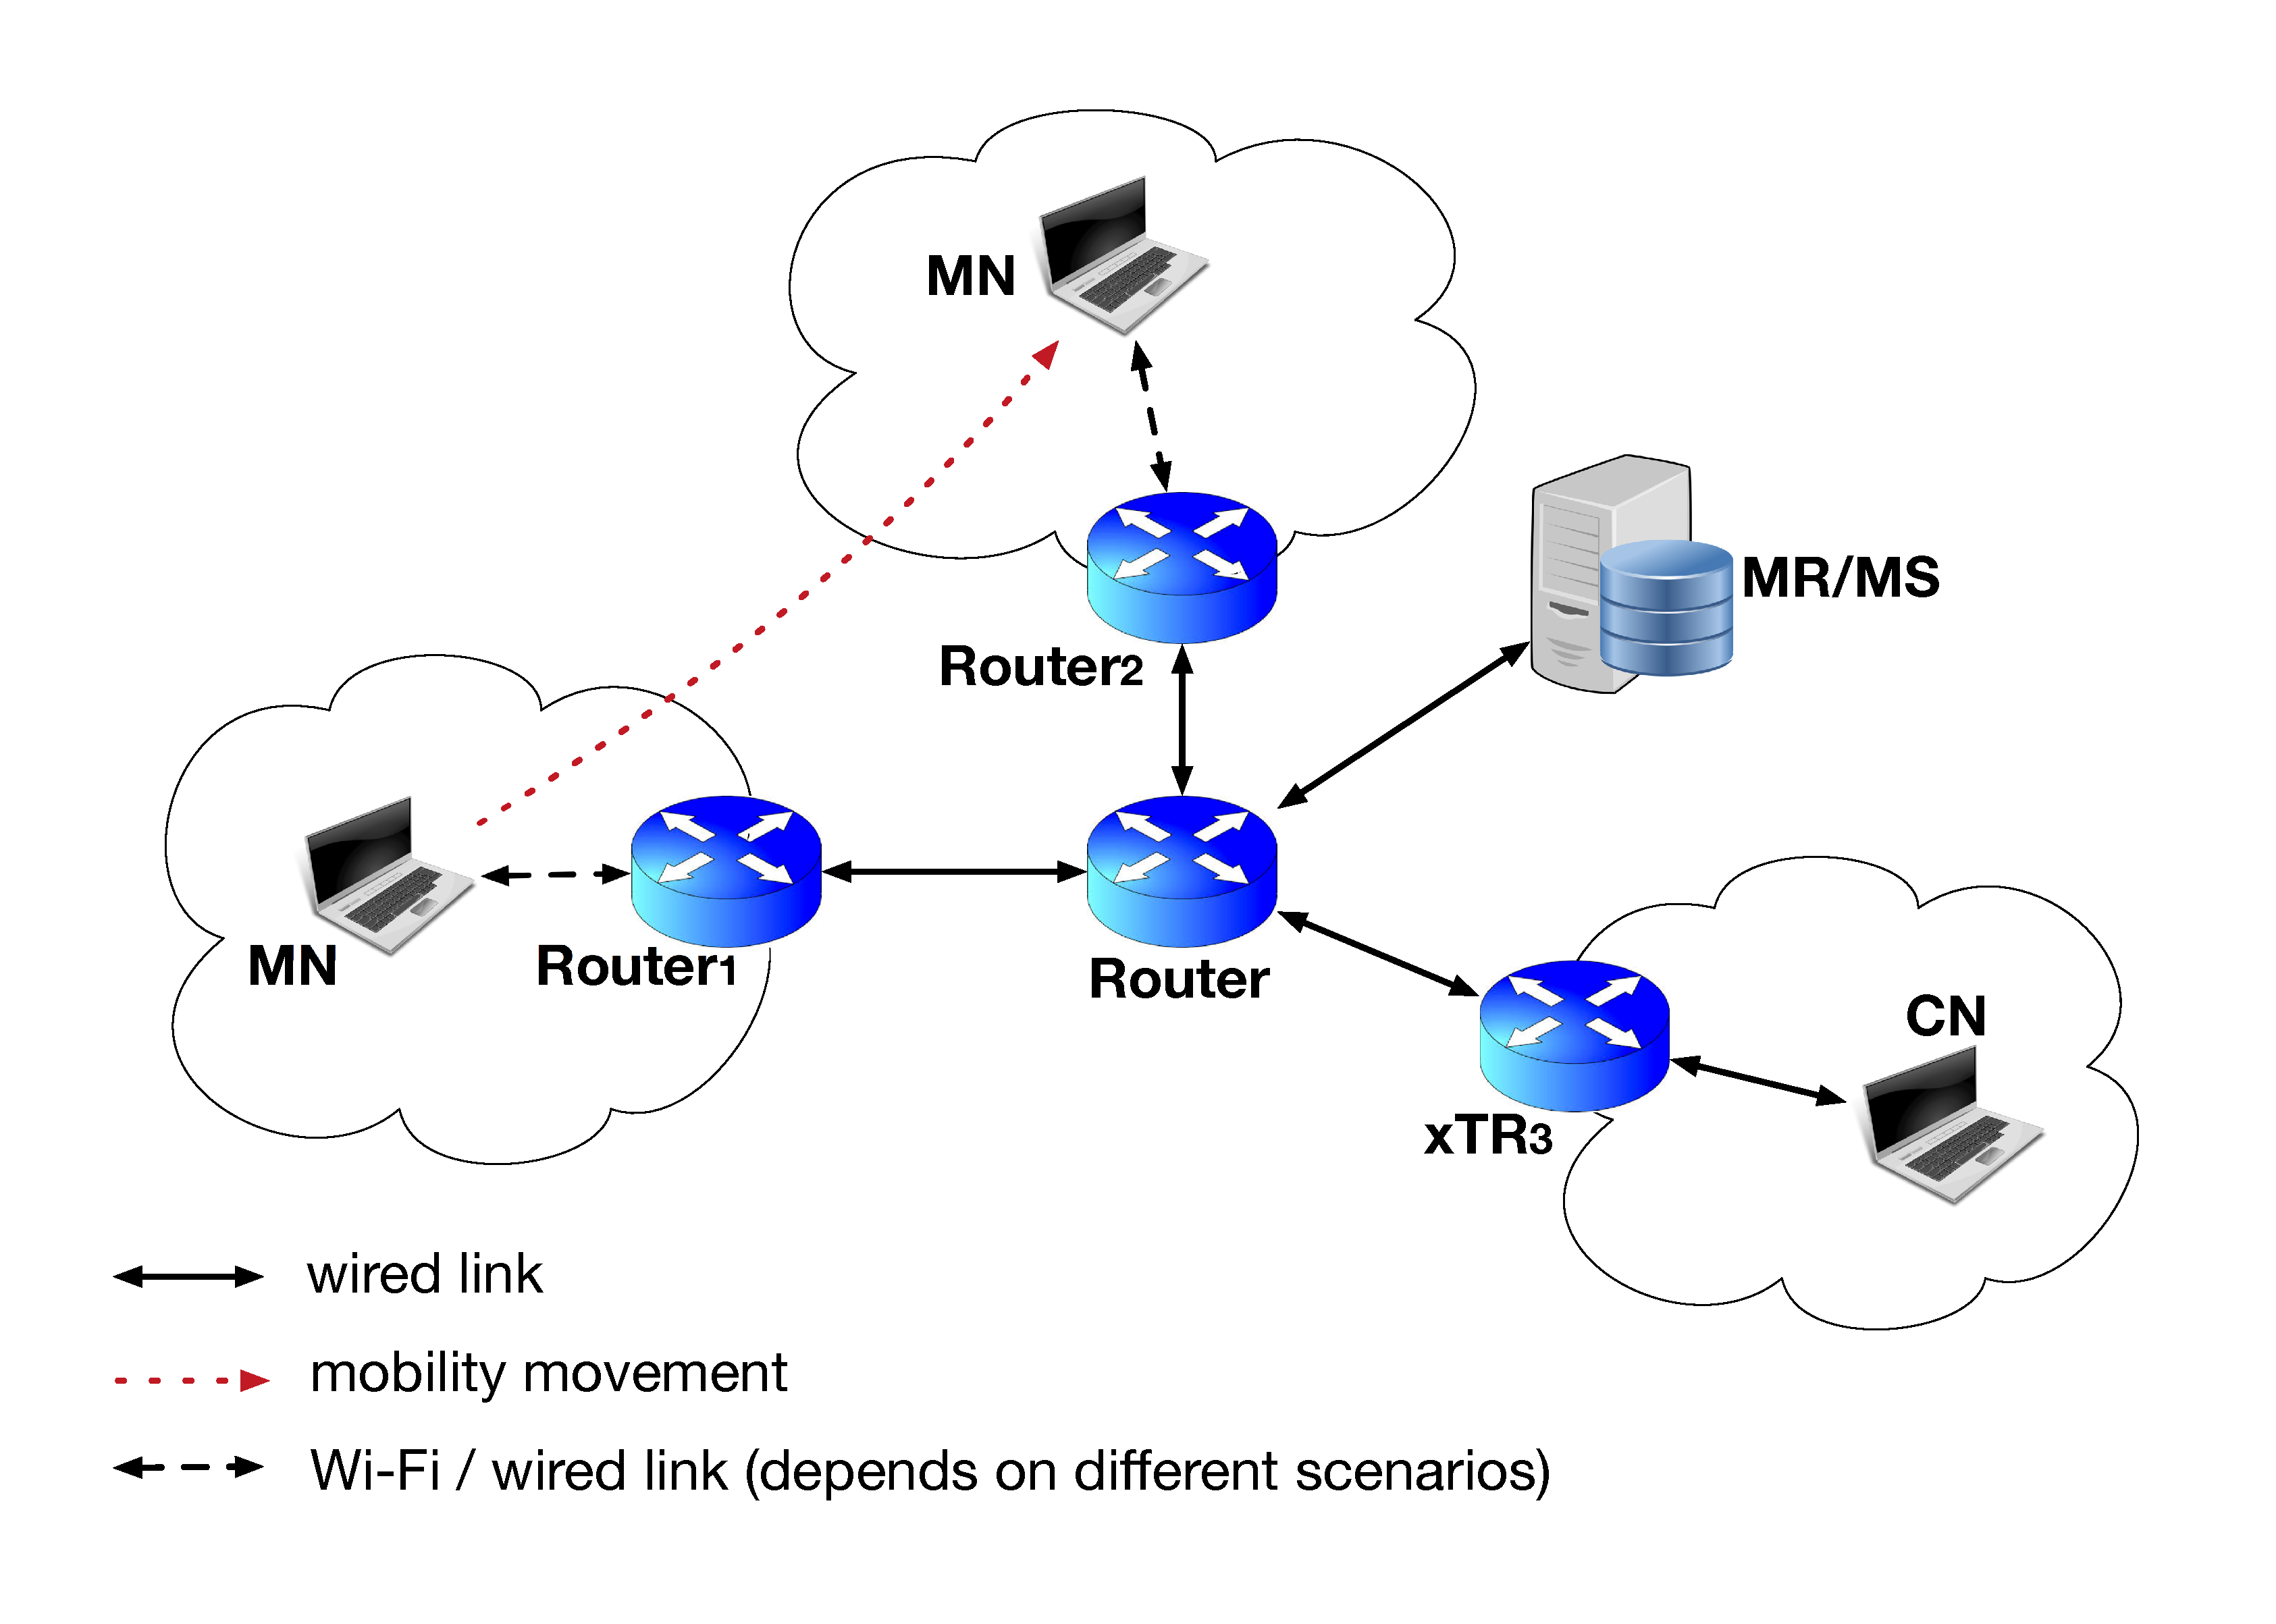
\includegraphics[width=0.8\textwidth]{Pics/LISP_mobility_archi}
	\caption{General scenario for LISP mobility architecture}
	\label{sim_archi}
\end{figure}
%-< END FIGURE >--------------------------------------------------------------------

% -<Descriptions with parameters>--------------------------------------------------------------------
% All the scenarios are based on a same simulation architecture shown in Fig.~\ref{sim_archi}, but with some slight differences, which will be respectively specified in the following parts from Sec.~\ref{sec:ns3_analysis_lispmn} to Sec.~\ref{sec:ns3_analysis_lispmn_xTR}. In our designed architecture, an MN is initially in the subnet of $Router_1$. An \emph{echo} application on MN sends packets to a remote stationary node CN in the LISP-Site of $xTR_3$. The distance between xTR\_1 and xTR\_2 is $170 m$. The connection between MN and xTR\_1 can be either Wi-Fi or wired link. If they use Wi-Fi, MN will move into the subnet of $Router_2$ at speed of $7.07 m/s$ after several seconds when the simulation begins. The start time of movement is a random value in the range of $[x, x] s$. At a certain moment during the moving, the Wi-Fi link between MN and $Router_1$ is down, which triggers the handover procedure. Afterwards, MN connects to $Router_2$ and reestablishes the communication with CN node. If they use wired link, the connection of MN with $Router_1$ will be down and the one with $Router_2$ will be up at the same time. This action also triggers the handover procedure. Every link between two network entities in this simulation architecture is set to $20 ms$.

The network topology for all the scenarios is shown in Fig.~\ref{sim_archi}. An MN is initially in the subnet of $Router_1$. It exchanges packets with a remote stationary node CN situated in the LISP-Site of $xTR_3$. The roles of $Router_1$ and $Router_2$ are slightly different in different scenarios. This will be respectively specified in the following parts (Sec.~\ref{sec:ns3_analysis_lispmn} to Sec.~\ref{sec:ns3_analysis_lispmn_xTR}). To obtain the estimation of LISP mobility handover, we do not consider the delay due to wireless link switch and use an intermediate router to connect all three routers and the mapping system. The connection between MN and $Router_1$ can be either Wi-Fi or wired link. If Wi-Fi link is used, MN will move into the subnet of $Router_2$ at a constant speed. At a certain moment, the Wi-Fi link between MN and $Router_1$ is down, which triggers the handover procedure. Afterwards, MN connects to $Router_2$ and re-establishes the communication with CN node. If they use wired link, the handover procedure can be simulated as follows. The MN have two interfaces respectively connected to $Router_1$ and $Router_2$. At a certain time, the connection to $Router_1$ set to be down and the one with $Router_2$ is set to be up. At the same time, the DHCP client on the interface connected to $Router_2$ is run and this triggers the handover procedure. By using wired link between MN and its routers is just to test the different mechanisms in an ideal situation, and it is not a real scenario.

In this chapter, the overall handover delay related to LISP $D_{overall}$ is defined as the time interval between the first and the last LISP packets during the handover procedure. % last packet received by MN from CN via $Router_1$ and the first packet received by MN from CN via $Router_2$ after the link reestablishment. 
The overall handover overhead $C_{overall}$ is defined as the number of LISP Control Plane messages exchanged during handover procedure.
According to the three following scenarios, the handover delay and overhead consist of different parts. All the necessary delay and LISP overhead of LISP Control Plane during the mobility are listed in Tab.~\ref{Symbols_numerical_analysis}.
%-< TABLE >-----------------------------------------------------------------
\begin{table}[!tb]
	\centering
	\caption{Symbols for numerical analysis}
	\label{Symbols_numerical_analysis}{
		% \resizebox{0.9\textwidth}{!}{%
		\begin{tabular}{@{}|c|c|@{}}
			\hline\hline
			Symbols & Explanations   \\ \hline
			$D_{overall}$ & Overall handover delay related to LISP	\\  \hline    
			$D_{DHCP}$ &  DHCP address configuration delay \\  \hline    
			$D_{Register}$ &  Delay of sending Map-Register      	\\  \hline
			$D_{Notify}$ &  Delay of receiving Map-Notify      	\\  \hline           
			$D_{Request}$ &  Delay of sending Map-Request to MDS      	\\  \hline   
			$D_{Reply}$ &  Delay of receiving Map-Reply      	\\  \hline      
			$D_{Resolve}$ &  Delay of resolving mapping information in MDS      	\\  \hline               
			$D_{SMR}$ &  Delay of sending SMR       	\\  \hline 
			$D_{Request_{SMR}}$ &  Delay of sending a SMR-invoked Map-Request \\  \hline 
			$D_{Link}$ &  Link delay between two network entities \\  \hline 
			$T_{A-B}$ &  Delay of packet transmission between A and B     	\\  \hline
			$T_{timeout_SMR}$ &  Timeout of SMR \\  \hline  \hline    
		\end{tabular}
	}
\end{table}
%-< END TABLE >-----------------------------------------------------------------



%-< SUBSECTION >--------------------------------------------------------------------
\subsection{LISP-MN in non-LISP-Site}
\label{sec:ns3_analysis_lispmn}
The first scenario is the LISP-MN in non-LISP-Site, where the border routers are the conventional routers and LISP is only implemented on the mobile end host MN. In our simulation, the LISP-MN with permanent EID is initially placed in the subnet of $Router_1$, with the IP address distributed by $Router_1$ as its RLOC. The remote CN is a conventional stationary end host, residing in a LISP-Site of $xTR_3$. % The LISP-MN communicates with CN by encapsulating the packets on itself and decapsulating the packets on $xTR_3$. If we use Wi-Fi, the LISP-MN moves into subnet of $Router_2$ after the simulation begins. At a certain moment during the moving, the Wi-Fi link between LISP-MN and $Router_1$ is down, whereas LISP-MN detects $Router_2$, which triggers the handover procedure. If we use wired link, after a certain time that the simulation begins, we turn down the wired link between LISP-MN and $Router_1$, while set the link between LISP-MN and $Router_2$ up at the same time. 
LISP-MN first has a DHCP procedure when MN moves to $Router_2$, so that the later allocates a new IP address as RLOC. Then LISP-MN needs register its new mapping information to the mapping system, and also send a $SMR$ to its communicating nodes in its cache (there is only CN in our scenario). $xTR_3$ sends an SMR-invoked Map-Request to the mapping system, so to obtain the new mapping information of LISP-MN. Afterwards, LISP-MN re-establishes  the communication with CN node via $Router_2$. The detailed traffic schema related to the handover procedure is illustrated in Fig.~\ref{sim_schema_LISPMN}.  % The total simulation time is set to $45s$ and the DHCP procedure delay is set to $1s$. We conduct many times of simulations with the various beacon interval of Wi-Fi channel in the range of $0.05s$ to $2s$.
%-< FIGURE >--------------------------------------------------------------------
\begin{figure}[!t]
	\centering
	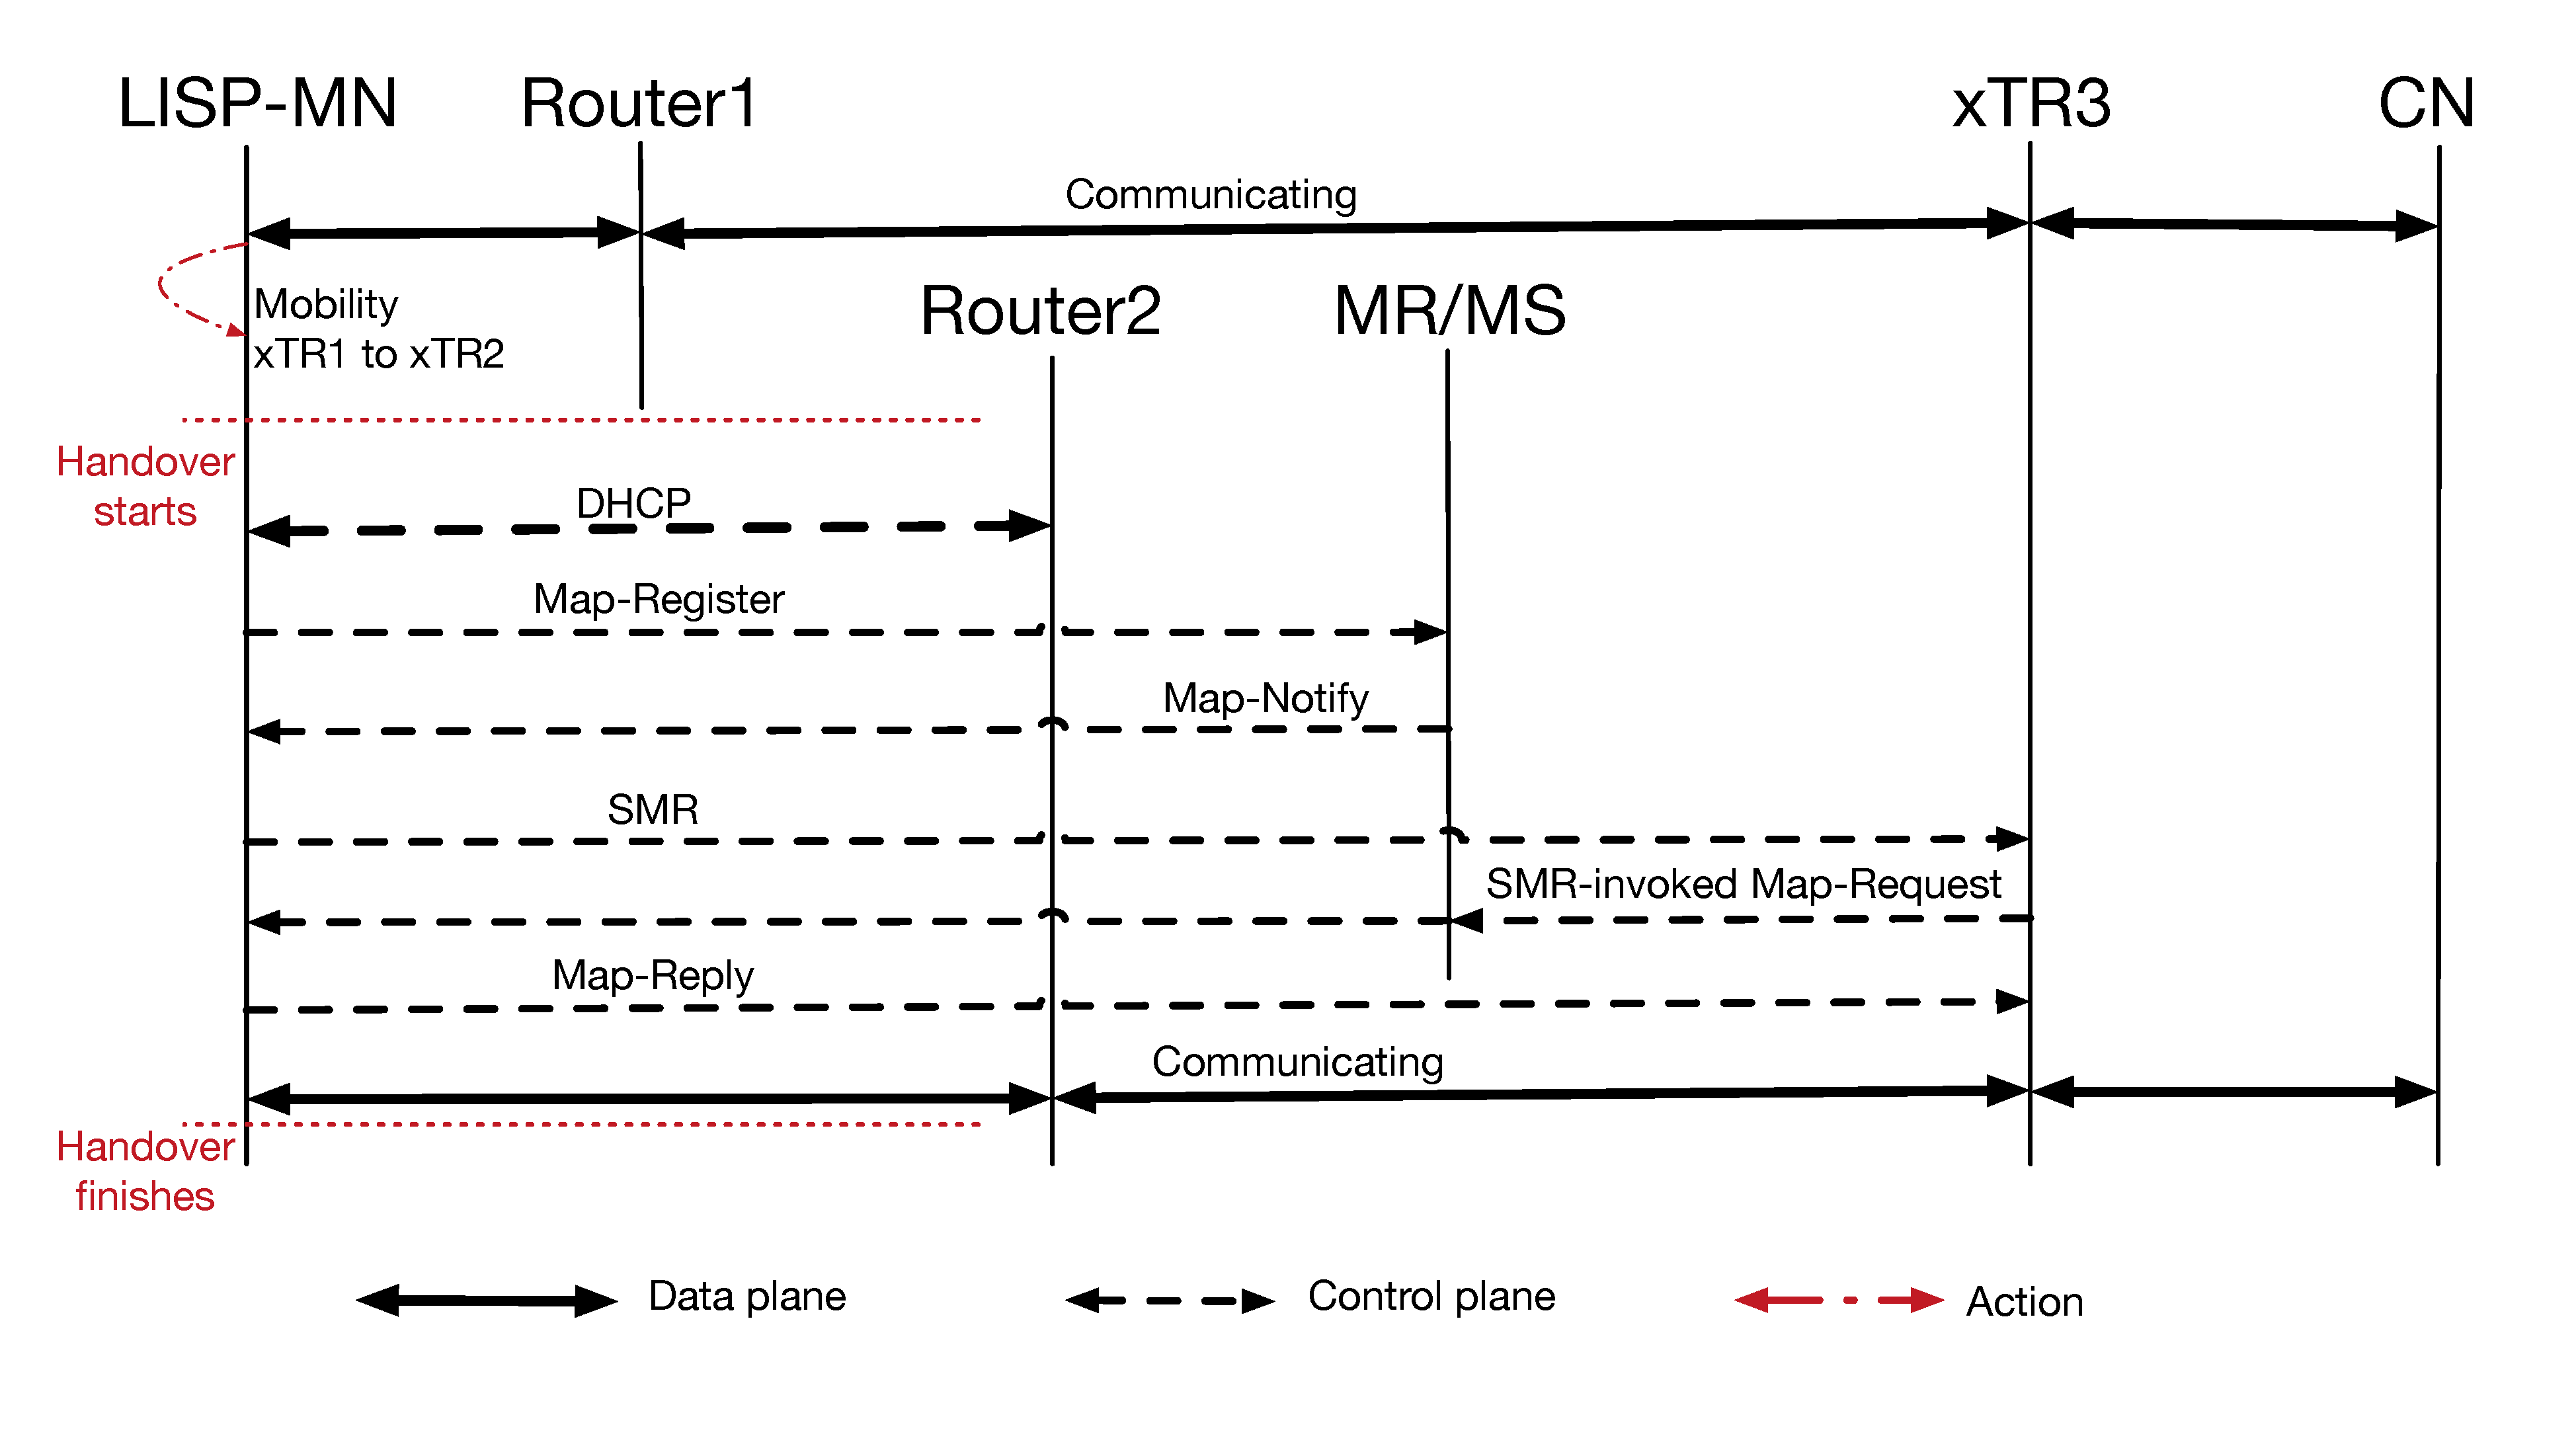
\includegraphics[width=0.8\textwidth]{Pics/Mobility_LISPMN_schema_SMR_simplify}
	\caption{Schema for LISP-MN mobility in non-LISP-Site (SMR-invoked Map-Request is sent to the mapping system)}
	\label{sim_schema_LISPMN}
\end{figure}
%-< END FIGURE >--------------------------------------------------------------------

The overall handover delay in this scenario is composed by two parts: the DHCP related delay and LISP related delay. The delays of DHCP procedures consist of LISP-MN sending DHCP Discovery message to $Router_2$, receiving DHCP Offer message, sending DHCP Request message, and receiving DHCP ACK message. The delays of all the LISP procedures are presented in Fig.~\ref{sim_schema_LISPMN}. This chapter only focus on the delay caused by LISP. Thus, the overall handover delay $D_{overall}$ related to LISP of LISP-MN in non-LISP-Site is:
\begin{eqnarray}
D_{overall} &=& D_{Register} + D_{Notify} + D_{SMR} + D_{Request_{SMR}} + D_{Reply} 
\end{eqnarray}
To facilitate the comparison between each scenario, we provide the numerical results for the designed topology as shown in Fig.~\ref{sim_archi}. Every link between two network entities in this architecture is set to $1 ms$. According to the experimental results of Coras et al.'s paper~\cite{coras2014performance}, we set the resolving time in the mapping system as $200 ms$. Thus, the $D_{overall}$ of the first scenario in our designed architecture is:
\begin{eqnarray}
% &=& T_{MN-MDS} + T_{MDS-MN} + T_{MN-xTR_3} + (T_{xTR_3-MDS} + D_{Resolve} + T_{MDS-MN}) + T_{MN-xTR_3} \nonumber \\
D_{overall} &=& 3T_{MN-MDS} + 2T_{MN-xTR_3} + T_{xTR_3-MDS} + D_{Resolve} \nonumber \\
&=& 3* (3*D_{Link}) + 2*(3*D_{Link}) + 2*D_{Link} + D_{Resolve}\nonumber \\
% &=& 3* (3*1ms) + 2*(3*1ms) + 2*1ms + D_{Resolve} \nonumber \\
&=& 17D_{Link} + D_{Resolve} \nonumber \\
&=& 217 ms \nonumber
\end{eqnarray}
% (Min value of handover delay = 1.073031 s, where packet sending interval = 0.01 s)

The handover overhead is 6 messages of LISP Control Plane. It includes 2 signalings of registration when LISP-MN connects to $Router_2$ (Map-Register and Map-Notify), and 4 signalings related to SMR procedure: 1 SMR from LISP-MN to $xTR_3$, 1 SMR-invoked Map-Request from $xTR_3$ to the mapping system, 1 Map-Request forwarded by mapping system to LISP-MN, and 1 Map-Reply from LISP-MN to $xTR_3$.
%\begin{eqnarray}
%C_{overall} &=& C_{Register} + C_{Notify} + C_{SMR} + C_{Request_{SMR}} + C_{Reply} \nonumber \\
%&=& C_{Register} + C_{Notify} + C_{SMR} + 2C_{Request} + C_{Reply} \nonumber \\
%&=& 6 C
%\end{eqnarray}

There are two options when $xTR_3$ receives $SMR$. It can send the SMR-invoked Map-Request to the mapping system as we described before, or it can directly send the SMR-invoked Map-Request to the source locator address of $SMR$~\cite{rfc6830}. In this scenario, the source of $SMR$ is LISP-MN. Thus, the overall handover delay $D_{overall}$ in this scenario is as follows:
\begin{eqnarray}
D_{overall} &=& D_{Register} + D_{Notify} + D_{SMR} + D_{Request_{SMR}} + D_{Reply} 
\end{eqnarray}
The numerical result is:
\begin{eqnarray}
% &=& T_{MN-MDS} + T_{MDS-MN} + T_{MN-xTR_3} + T_{xTR_3-MN} + T_{MN-xTR_3} \nonumber \\
&=& 2T_{MN-MDS} + 3T_{MN-xTR_3}  \nonumber \\
&=& 2* (3*D_{Link}) + 3*(3*D_{Link}) \nonumber \\
% &=& 2* (3*1ms) + 3*(3*1ms) \nonumber \\
&=& 15D_{Link} \nonumber \\
&=& 15 ms \nonumber
\end{eqnarray}
Compared with solution of sending SMR-invoked Map-Request to the mapping system, the overall handover delay of sending the SMR-invoked Map-Request back to the source of $SMR$ is smaller, since there is no resolving delay in the mapping system. % This solution is more interesting for the case that the distance to mapping system is much longer than that to the source of $SMR$.

In this scenario, the handover overhead associated to LISP Control Plane is 5 messages. Since the SMR-invoked Map-Request is directly sent from $xTR_3$ to LISP-MN instead of passing the mapping system, it has 1 signaling less than the one sent to the mapping system.
%\begin{eqnarray}
%C_{overall} &=& C_{Register} + C_{Notify} + C_{SMR} + C_{Request_{SMR}} + C_{Reply} \nonumber \\
%&=& C_{Register} + C_{Notify} + C_{SMR} + C_{Request} + C_{Reply} \nonumber \\
%&=& 5 C
%\end{eqnarray}

The advantages of this scenario, i.e., LISP-MN in non-LISP-Site, are: 
\begin{inparaenum}[1)]
	\item it is able to achieve handover through different subnets;
	\item the numerical analysis indicates that the overall handover delay is small;
	\item so to the overall overhead. Compared to the other two scenarios, which will be described in details in the following sections, the mobility in this scenario does not cause lots of traffic in LISP Control Plane.
\end{inparaenum}
However, since the routers are still the normal routers in this scenario, it cannot help to reduce the BGP routing table size, which is the initial purpose to motivate LISP. Moreover, each LISP-MN needs a permanent IP address as its EID, which increases the burden of IPv4 address allocation. Each permanent EID and its LRLOC needs register to the mapping system, which also increases the size of LISP mapping table.

%-< SUBSECTION >--------------------------------------------------------------------
\subsection{MN in LISP-Site}
\label{sec:ns3_analysis_xTR}
The second scenario is the MN in LISP-Site, where the mobile node MN is conventional and LISP are only implemented on the border routers. In our simulation, the MN is initially placed in the subnet of $xTR_1$, with the assigned IP address as its EID. The remote CN is same to the first scenario. The MN communicates with CN by encapsulating the packets on $xTR_1$ and decapsulating the packets on $xTR_3$, and the MN moves into the coverage of $xTR_2$ after the simulation begins. Since the communication should not be interrupted during the mobility, this scenario limits the movement of MN being only within the same subnet, i.e., one of the EID-prefixes of $xTR_1$ is same to one of $xTR_2$'s. % At a certain moment during the moving, the Wi-Fi link between MN and $xTR_1$ is down, whereas MN detects $xTR_2$, which triggers the switching connection procedure. If we use wired link, after a certain time that the simulation begins, the wired link between MN and $xTR_1$ is down, meanwhile the link between MN and $xTR_2$ is up. 
Similar to the first scenario, the DHCP procedure is necessary so to trigger the registration of new mapping information, but MN still keeps the former IP address as its EID, instead of $xTR_2$ distributing a new one to it. Then $xTR_2$ registers the new mapping information to the mapping system. As the mapping system finds out that the EID of MN has been registered and associated by $xTR_1$, it sends a Map-Notify to both xTRs. The reason for sending to $xTR_2$ is the acknowledgment of the reception of its Map-Register. Whereas the purpose to $xTR_1$ is to tell it that the MN is now mapping with $xTR_2$ and inform the remote CN to update its mapping information. Since MN used $xTR_1$ to communicate with CN in the past time, only $xTR_1$ stored in its cache that to whom MN was exchanging the packets instead of $xTR_2$. Thus, $xTR_1$ sends a $SMR$ to $xTR_3$, and $xTR_3$ sends an SMR-invoked Map-Request to the mapping system, so to obtain the new mapping information of MN. Afterwards, MN re-establishes the communication with CN node via $xTR_2$. The detailed traffic schema related to the handover procedure is shown in Fig.~\ref{sim_schema_xTR}.
%-< FIGURE >--------------------------------------------------------------------
\begin{figure}[!t]
	\centering
	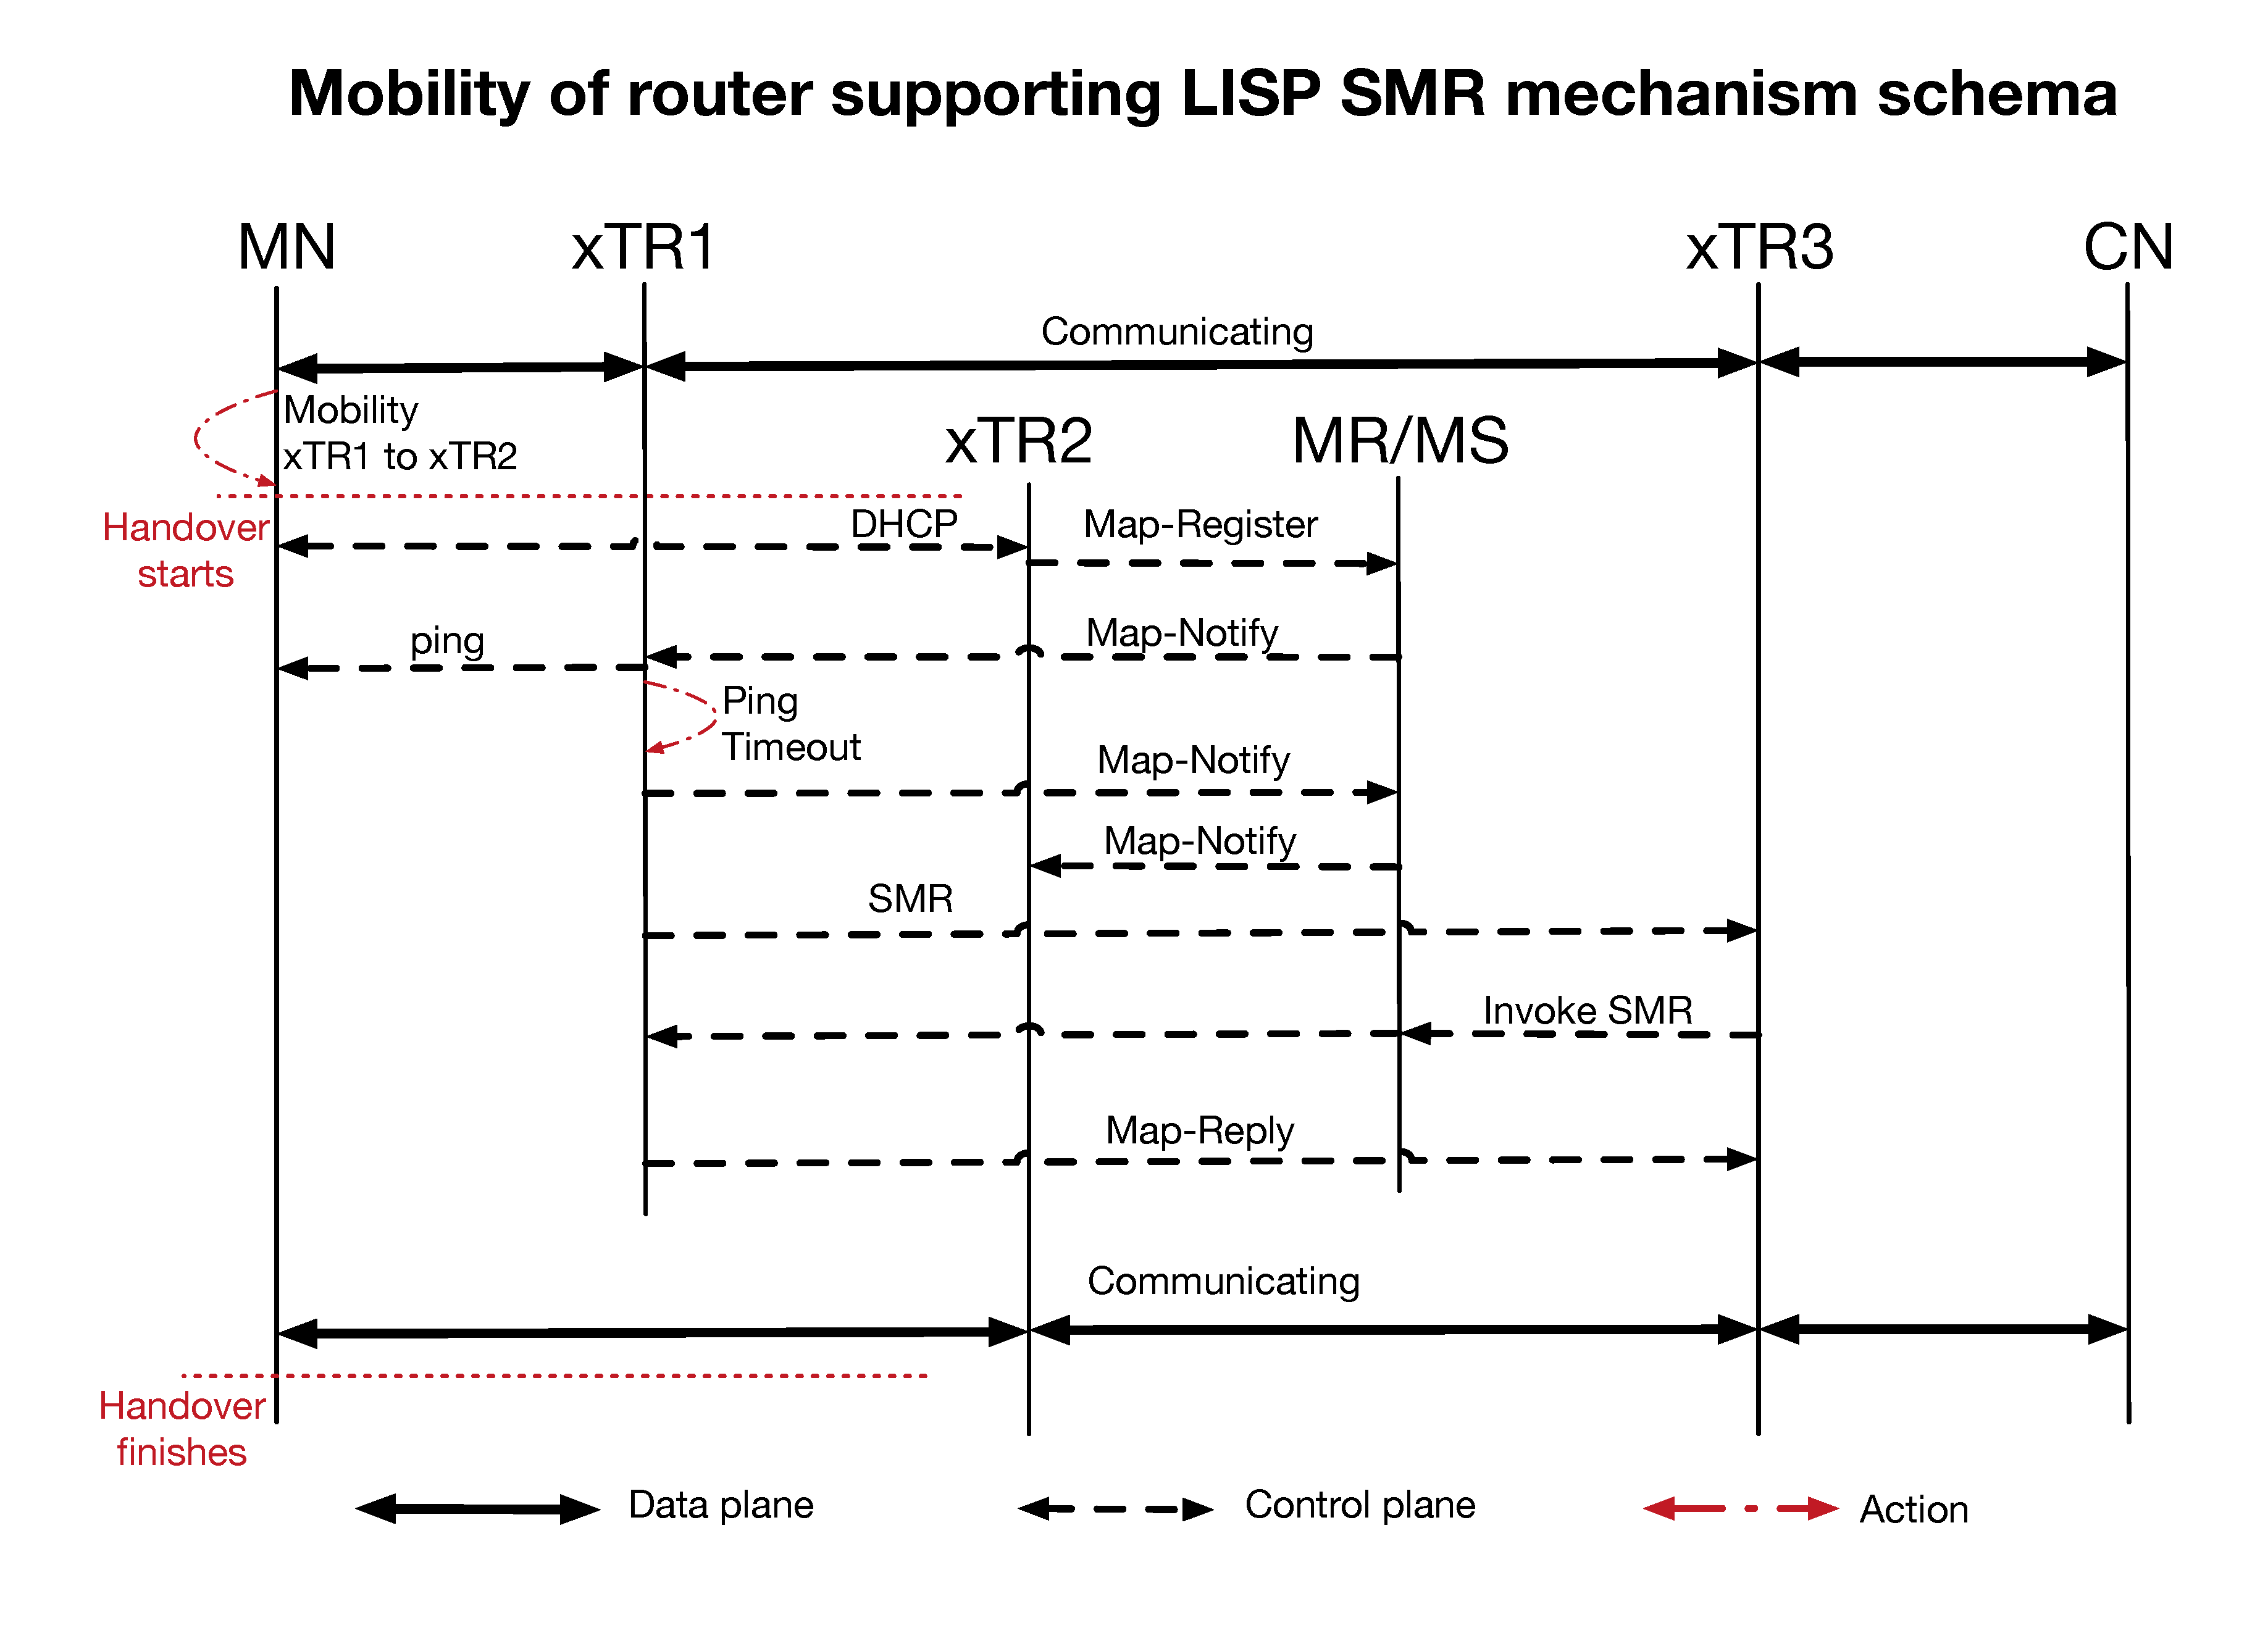
\includegraphics[width=0.8\textwidth]{Pics/Mobility_xTR_schema_SMR_simplify}
	\caption{Schema for MN mobility in LISP-Site (SMR-invoked Map-Request is sent to the mapping system)}
	\label{sim_schema_xTR}
\end{figure}
%-< END FIGURE >--------------------------------------------------------------------

The overall handover delay $D_{overall}$ in this scenario is almost same to the first one:
\begin{eqnarray}
D_{overall} &=& D_{Register} + D_{Notify} + D_{SMR} + D_{Request_{SMR}} + D_{Reply} 
\end{eqnarray}
The numerical result is as follows:
\begin{eqnarray}
% &=& T_{xTR_2-MDS} + T_{MDS-xTR_1} + T_{xTR_1-xTR_3} + T_{xTR_3-MDS} + D_{Resolve} + T_{MDS-xTR_2} + T_{xTR_2-xTR_3} \nonumber \\
D_{overall} &=& 2T_{xTR_2-MDS} + T_{MDS-xTR_1} + T_{xTR_1-xTR_3} + T_{xTR_3-MDS} + \nonumber \\
& & D_{Resolve} + T_{xTR_2-xTR_3} \nonumber \\
&=& 2* (2*D_{Link}) + 2*D_{Link} + 2*D_{Link} + 2*D_{Link} + D_{Resolve} + 2*D_{Link} \nonumber \\
% &=& 2* (2*1ms) + 2*1ms + 2*1ms + 2*1ms + D_{Resolve} + 2*1ms \nonumber \\
&=& 12D_{Link} + D_{Resolve}  \nonumber \\
&=& 212 ms \nonumber
\end{eqnarray}
% $CheckAlive$ is the delay that xTR\_1 checks if MN still connects to it. For example, xTR\_1 can simply \emph{ping} MN. If MN still connects to it, it will reply to mapping system that itself is still RLOC of MN. Otherwise, if \emph{ping} meets timeout, xTR\_1 will tell the mapping system that MN has left, and sends SMR to the CNs in its cache. The later situation has higher delay, because xTR\_1 needs to wait until timeout of \emph{ping}. % (Min value of simulation = 1.067679 s, where includes 1 s of DHCP delay)

The handover overhead in this scenario is 7. Besides 4 messages used for SMR procedure, it needs 3 signalings to complete the registration. There are 1 Map-Register from $xTR_2$ to the mapping system and 2 messages of Map-Notify: 1 to the $xTR_2$ and 1 to the $xTR_1$.
%\begin{eqnarray}
%C_{overall} &=& C_{Register} + 2C_{Notify} + C_{SMR} + C_{Request_{SMR}} + C_{Reply} \nonumber \\
%&=& C_{Register} + 2C_{Notify} + C_{SMR} + 2C_{Request} + C_{Reply} \nonumber \\
%&=& 7 C
%\end{eqnarray}

Same to the first scenario having two options, when $xTR_3$ receives the $SMR$ from $xTR_1$, it can also directly send SMR-invoked Map-Request back to $xTR_1$, which implies that the $xTR_1$ puts the new mappings into its database. The overall handover delay $D_{overall}$ is as follows:
\begin{eqnarray}
D_{overall} &=& D_{Register} + D_{Notify} + D_{SMR} + D_{Request_{SMR}} + D_{Reply}
\end{eqnarray}
The numerical result is:
\begin{eqnarray}
% &=& T_{xTR_2-MDS} + T_{MDS-xTR_1} + T_{xTR_1-xTR_3} + T_{xTR_3-xTR_2} + T_{xTR_2-xTR_3} \nonumber \\
&=& T_{xTR_2-MDS} + T_{MDS-xTR_1} + T_{xTR_1-xTR_3} + 2T_{xTR_2-xTR_3} \nonumber \\
&=& 2*D_{Link} + 2*D_{Link} + 2*D_{Link} + 2*(2*D_{Link}) \nonumber \\
% &=& 2*1ms + 2*1ms + 2*1ms + 2*(2*1ms) \nonumber \\
&=& 10D_{Link}  \nonumber \\
&=& 10 ms \nonumber
\end{eqnarray}
Since the SMR-invoked Map-Request is not sent to the mapping system, there is no resolving delay. %, and the overall handover delay is much smaller than the former solution. 
However, in this scenario, as $xTR_1$ is no longer in charge of MN, how long it stores the CNs for MN in its cache is an important point to discuss. If the expired time is set too long, it wastes the source of $xTR_1$ and is not necessary. % Whereas if the time is too short, there is the risk that remote xTRs of CNs like $xTR_3$ in our scenario, do not have enough time to request the new mapping information. Thus, an optimal value of timeout that offers an appropriate tradeoff between saving the sources and effectively updating the new mapping information of remote remains an open question.
Thus, it still remains as an open issue to seek for an optimal value of timeout that offers an appropriate tradeoff between resources saving and effectively providing the new mapping information.

Same to the first scenario that directly responding to the source locator of SMR has 1 signaling less than the one requesting to the mapping system first. Thus, the overall handover overhead in this case is 6.
%\begin{eqnarray}
%C_{overall} &=& C_{Register} + 2C_{Notify} + C_{SMR} + C_{Request_{SMR}} + C_{Reply} \nonumber \\
%&=& C_{Register} + 2C_{Notify} + C_{SMR} + C_{Request} + C_{Reply} \nonumber \\
%&=& 6 C
%\end{eqnarray}

Since the routers support LISP, i.e., are the xTRs in this scenario, it can help to reduce the BGP routing table size, which is the initial motivation of proposing LISP. Besides, the analysis hints that the overall handover delay of this scenario is the shortest. However, it can only provide the mobility within a same subnet, which means that it is not able to offer the handover through different subnets. Thus, this scenario is more suitable to be applied for the mobility of virtual machines in the Data Center.

%-< SUBSECTION >--------------------------------------------------------------------
\subsection{LISP-MN in LISP-Site}
\label{sec:ns3_analysis_lispmn_xTR}
The third scenario is the LISP-MN in LISP-Site, where both the border routers and the mobile node MN are implemented LISP. In our simulation, the LISP-MN with permanent EID is initially placed in the subnet of $xTR_1$, with the IP address allocated by $xTR_1$ as its LRLOC. The remote CN is still same to the first two scenarios, which is a conventional stationary end host, residing in a LISP-Site of $xTR_3$. The LISP-MN communicates with CN by double encapsulation. The first encapsulation is on itself and the second time is on the $xTR_1$. When the LISP packets arrive at $xTR_3$, it needs decapsulate them twice. % If we use Wi-Fi, the LISP-MN moves into subnet of $xTR_2$ after the simulation begins. At a certain moment during the moving, the Wi-Fi link between LISP-MN and $xTR_1$ is down, whereas LISP-MN detects $xTR_2$, which triggers the handover procedure. If we use wired link, after a certain time that the simulation begins, we turn down the wired link between LISP-MN and $xTR_1$, while set the link between LISP-MN and $xTR_2$ up at the same time. 
LISP-MN first has a DHCP procedure with $xTR_2$, so that the later assigns it a new IP address as its LRLOC. Then LISP-MN needs register its new mapping information to the mapping system, and also send a $SMR$ to all the xTRs of CNs in its cache (actually is to the xTR of CN, i.e., $xTR_3$ in our scenario). Once $xTR_3$ receives a $SMR$, it sends an SMR-invoked Map-Request to the mapping system, so to obtain the new mapping information of LISP-MN. Actually, this mapping information that $xTR_3$ obtains is the $<EID_MN, LRLOC>$ for LISP-MN. It is not able to send the packets to LISP-MN at the moment, since it does not know how to route the packets to the $LRLOC$ of LISP-MN, i.e., it lacks the mapping information for $LRLOC$. Only until $xTR_3$ receives the packets from CN to LISP-MN, which triggers the Map-Request procedure to the mapping system, can $xTR_3$ know the mapping information of LRLOC $<LRLOC, RLOC_{xTR_2}>$. Now $xTR_3$ gets the double mapping information for LISP-MN. Afterwards, LISP-MN re-establishes  the communication with CN node by passing $xTR_2$. The detailed traffic schema related to the handover procedure is illustrated in Fig.~\ref{Mobility_double_encap_schema_SMR_askMDS_simplify}.

Since this scenario is double encapsulation that $xTR_3$ needs to know both inner and outer mapping information of LISP-MN for sending the packets. The overall handover delay $D_{overall}$ in this scenario is larger than the first two scenarios. The $D_{overall}$ is:
\begin{eqnarray}
D_{overall} &=& D_{Register} + D_{Notify} + D_{SMR} + D_{Request_{SMR}} + D_{Reply} +  \nonumber \\
& & D_{Request}+ D_{Reply} 
\end{eqnarray}
The numerical result is as follows:
\begin{eqnarray}
% &=& 2T_{MN-MDS} + T_{MN-xTR_3} + T_{xTR_3-MDS} + D_{Resolve} + T_{MDS-MN} + T_{MN-xTR_3} + T_{xTR_3-MDS} + D_{Resolve} + T_{MDS-xTR_2} + T_{xTR_2-xTR_3}   \nonumber \\
&=& 3T_{MN-MDS} + 2T_{MN-xTR_3} + 2T_{xTR_3-MDS} + 2D_{Resolve} +   \nonumber \\
& & T_{MDS-xTR_2} + T_{xTR_2-xTR_3}   \nonumber \\
&=& 3* (3*D_{Link}) + 2*(3*D_{Link}) + 2*(2*D_{Link}) + 2D_{Resolve} +  \nonumber \\
& & 2*D_{Link} + 2*D_{Link} \nonumber \\
% &=& 3* (3*1ms) + 2*(3*1ms) + 2*(2*1ms) + 2D_{Resolve} +  \nonumber \\
% & & 2*1ms + 2*1ms \nonumber \\
&=& 23D_{Link} + 2D_{Resolve}   \nonumber \\
&=& 423 ms \nonumber
\end{eqnarray}
%-< FIGURE >--------------------------------------------------------------------
\begin{figure}[!t]
	\centering
	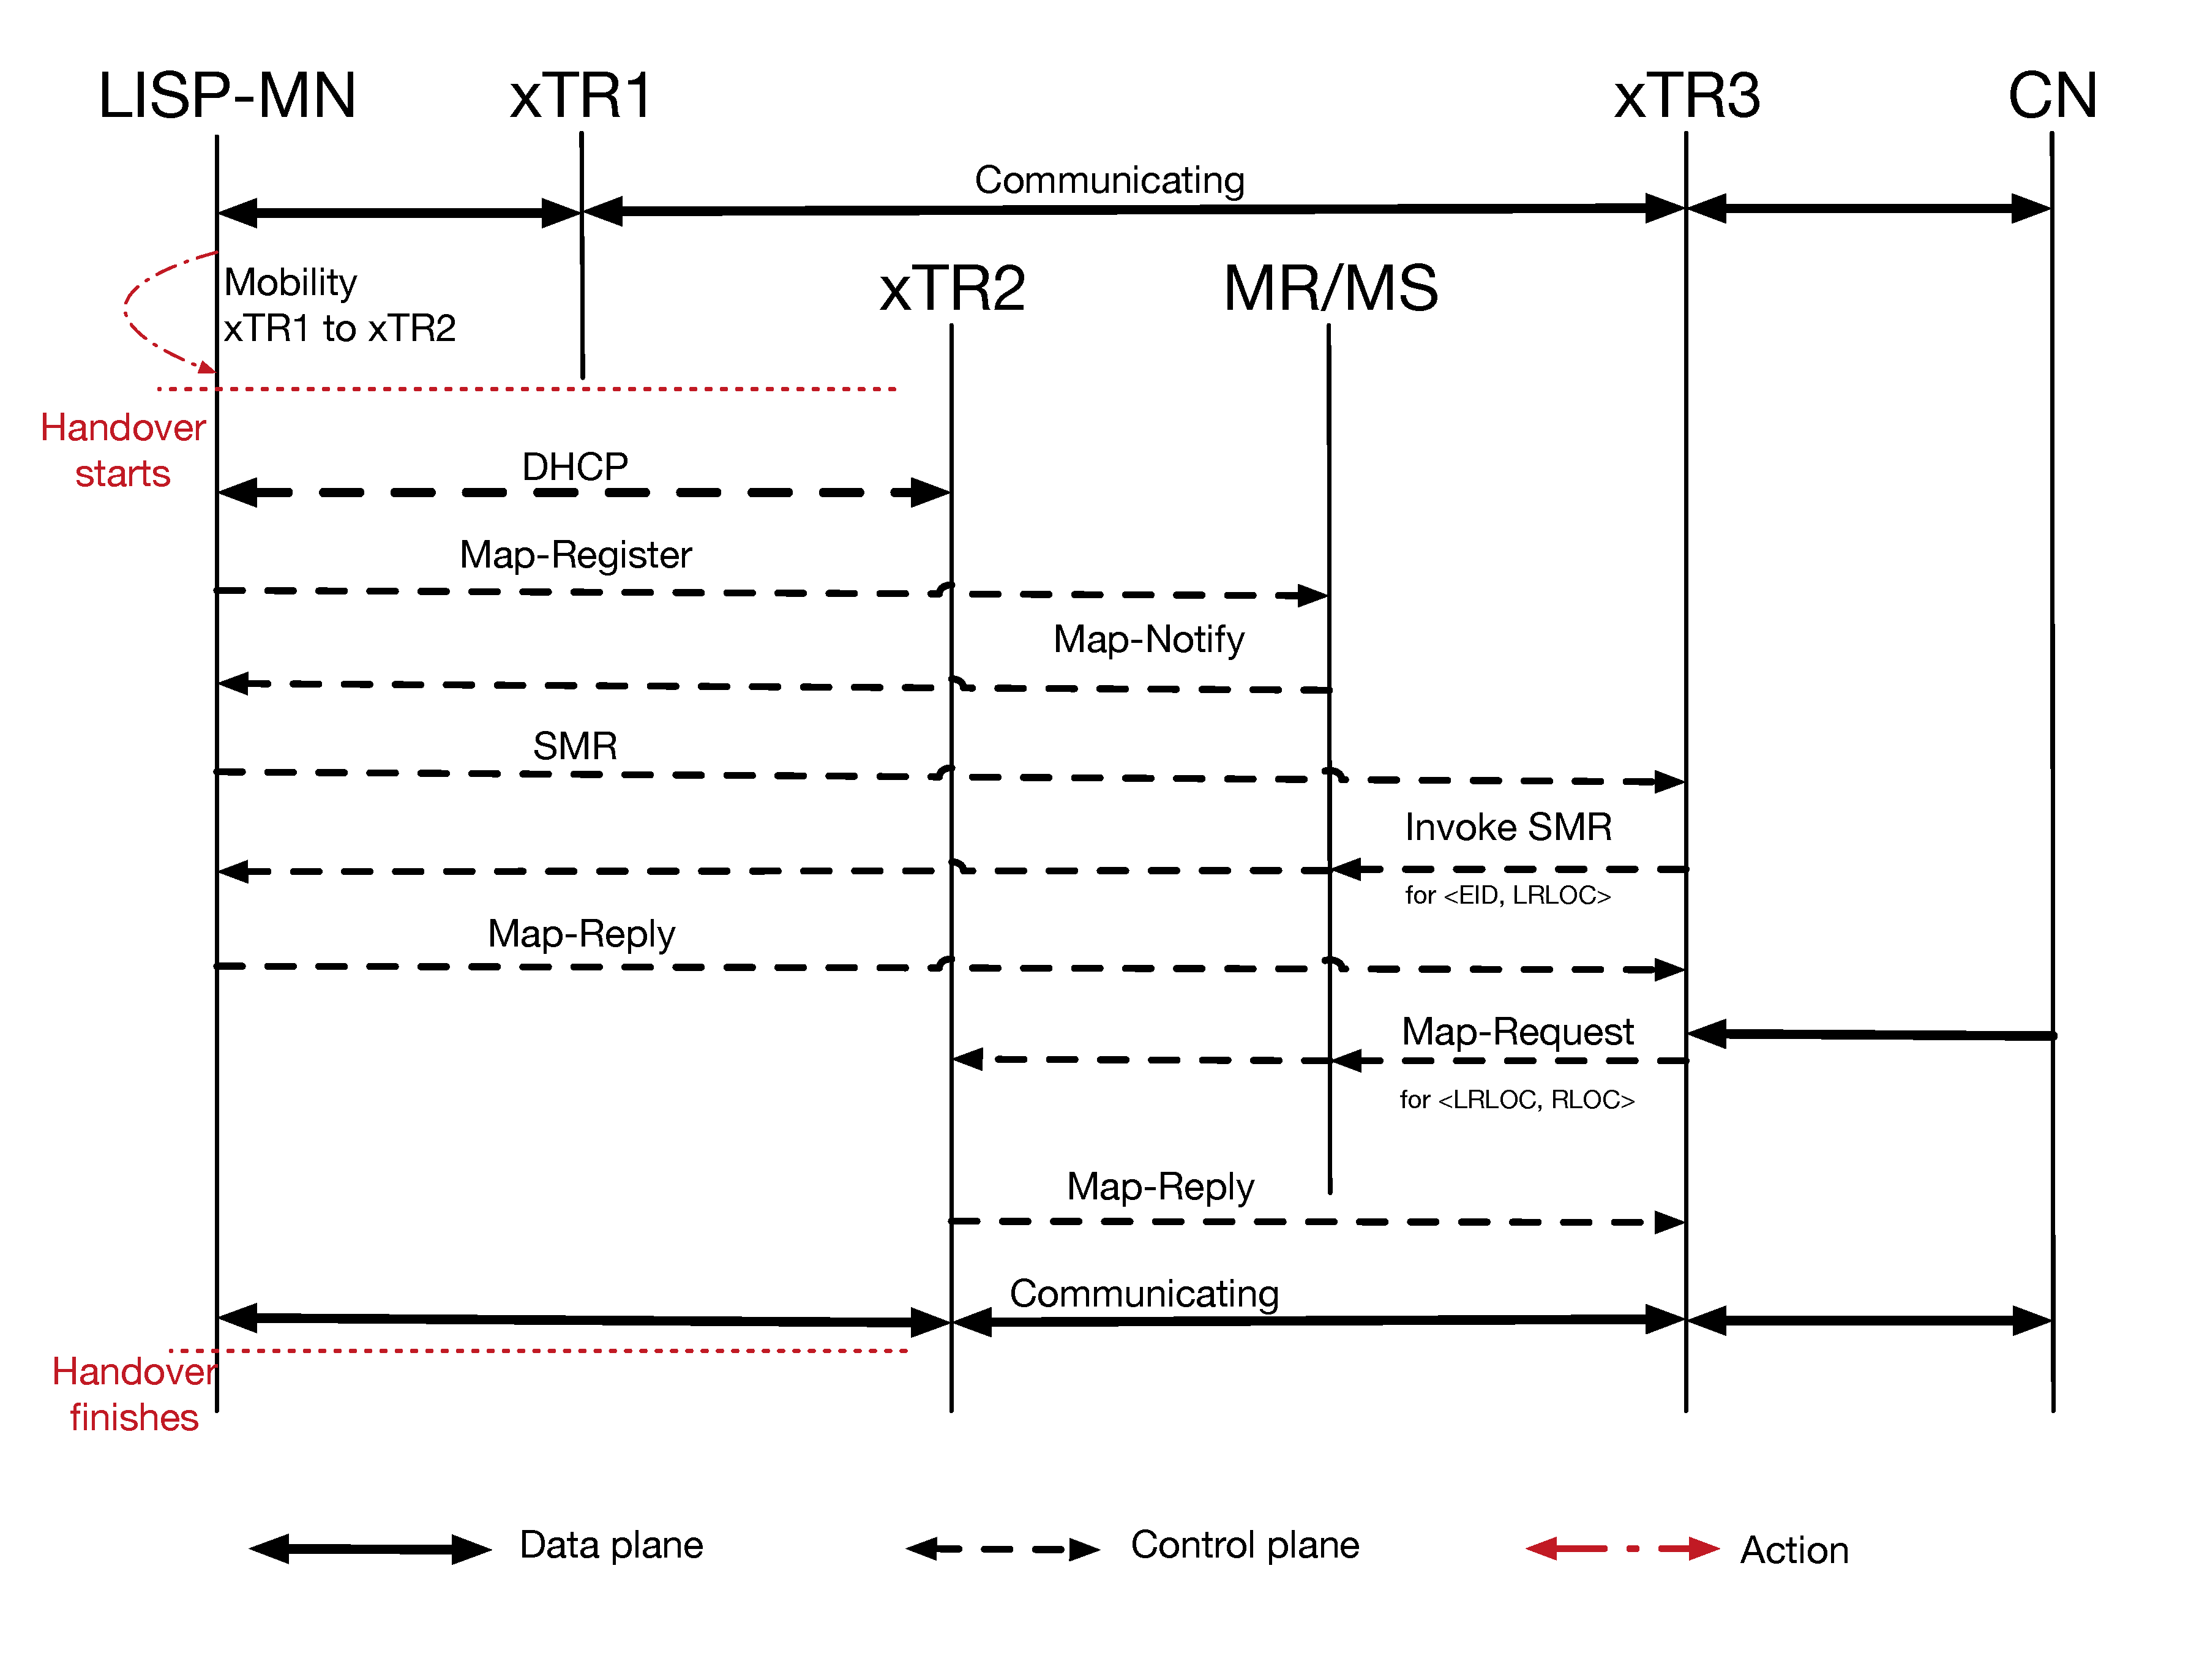
\includegraphics[width=0.8\textwidth]{Pics/Mobility_double_encap_schema_SMR_askMDS_simplify}
	\caption{Schema for LISP-MN mobility in LISP-Site (SMR-invoked Map-Request is sent to the mapping system)}
	\label{Mobility_double_encap_schema_SMR_askMDS_simplify}
\end{figure}
%-< END FIGURE >--------------------------------------------------------------------

The double encapsulation causes not only longer handover delay but also more handover overhead related to LISP Control Plane. Two messages are needed for the registration, 3 signalings are used to obtain the $LRLOC$ of $EID$. Besides, two more Map-Requests (one from $xTR_3$ to the mapping system, one from the mapping system to $xTR_2$) and one more Map-Reply are required to get the $RLOC$ of $LRLOC$. Thus, the handover overhead is 9, which has 3 messages more than the first scenario.
%\begin{eqnarray}
%C_{overall} &=& C_{Register} + C_{Notify} + C_{SMR} + C_{Request_{SMR}} + C_{Reply} + C_{Request} + C_{Reply} \nonumber \\
%&=& C_{Register} + C_{Notify} + C_{SMR} + 2C_{Request} + C_{Reply} + 2C_{Request} + C_{Reply} \nonumber \\
%&=& 9 C
%\end{eqnarray}

Differently from the first two scenarios, when $xTR_3$ directly sends the SMR-invoked Map-Request back to the source of $SMR$ has smaller overall handover delay, this solution for the third scenario has bigger delay instead. It is caused by the double encapsulation in this scenario while the first two scenarios have only single encapsulation. When $xTR_3$ receives the $SMR$ from LISP-MN, it wants to send SMR-Invoked Map-Request to the LISP-MN for the mapping information of $<EID_MN, LRLOC>$, but it does not know how to reach to LISP-MN, i.e., it lacks the mapping information of $<LRLOC, RLOC_{xTR_2}>$. Thus, it discards the $SMR$ and sends the Map-Request to the mapping system first. Then, the mapping information of $<LRLOC, RLOC_{xTR_2}>$ is stored in its cache. It waits for the next $SMR$ so to send the SMR-invoked Map-Request to the LISP-MN. The traffic schema is shown in Fig.~\ref{Mobility_double_encap_schema_SMR_askxTR_simplify}.
%-< FIGURE >--------------------------------------------------------------------
\begin{figure}[!t]
	\centering
	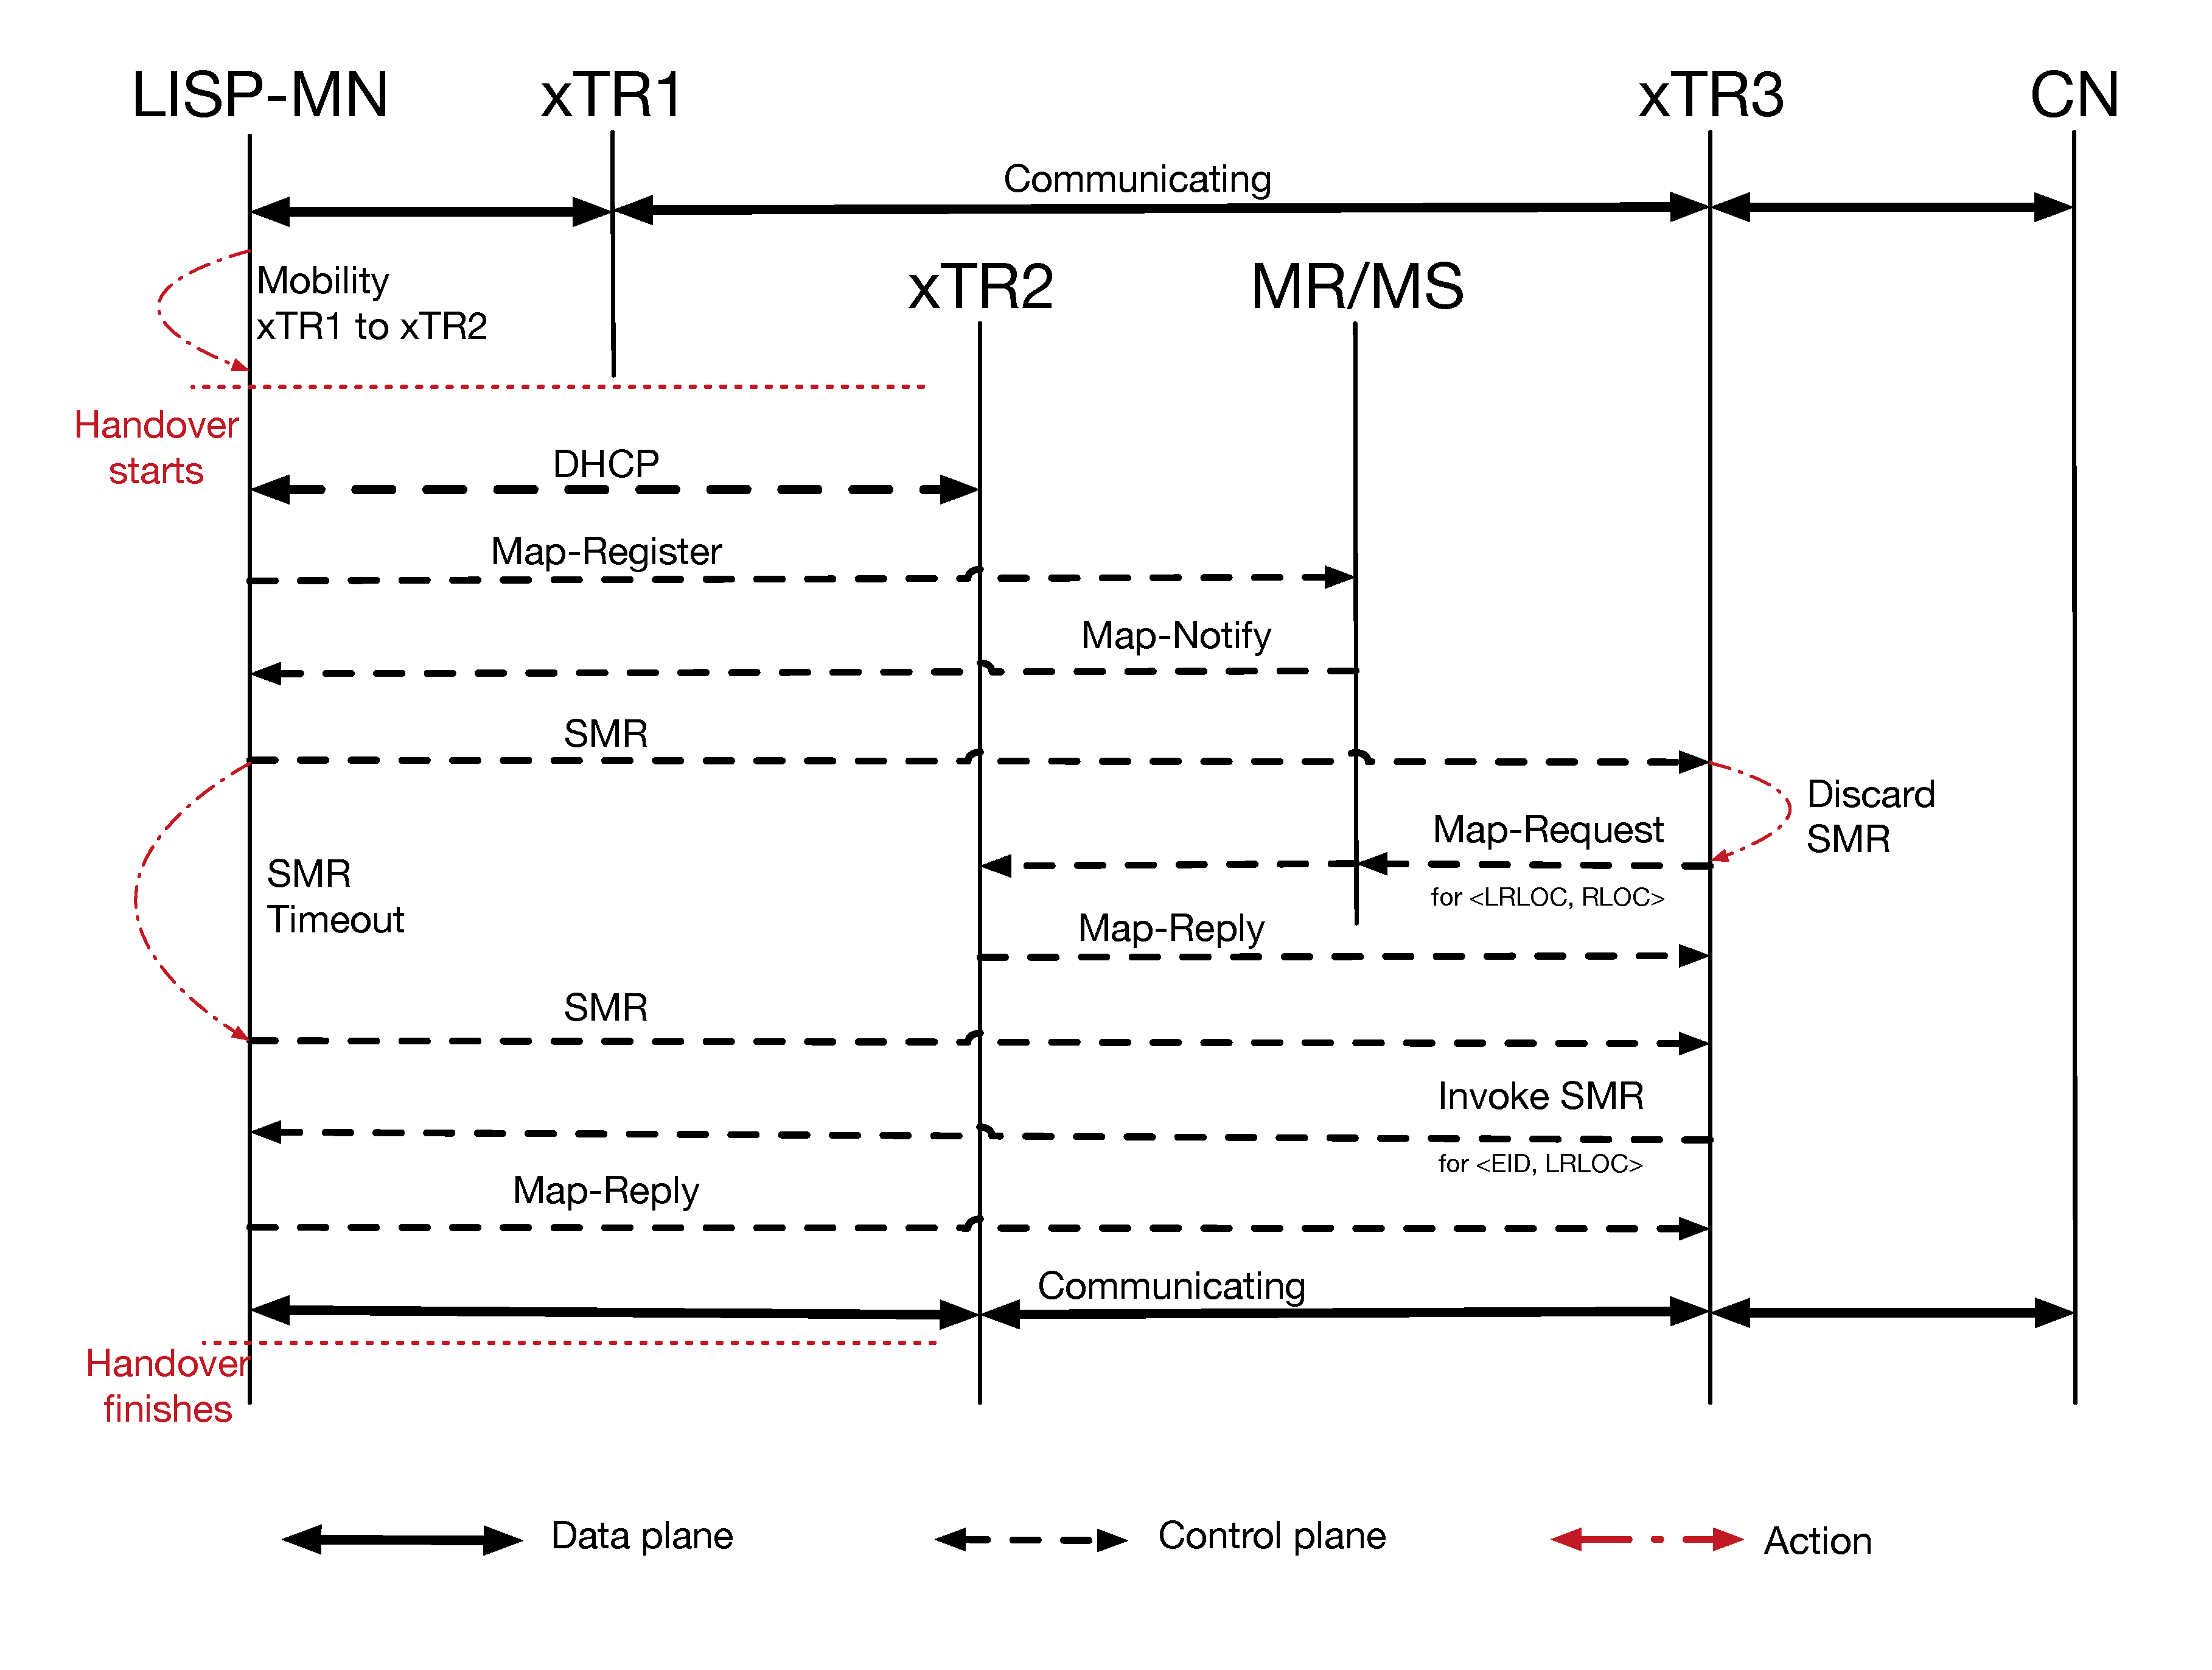
\includegraphics[width=0.8\textwidth]{Pics/Mobility_double_encap_schema_SMR_askxTR_simplify}
	\caption{Schema for LISP-MN mobility in LISP-Site (SMR-invoked Map-Request is sent to the source of SMR)}
	\label{Mobility_double_encap_schema_SMR_askxTR_simplify}
\end{figure}
%-< END FIGURE >--------------------------------------------------------------------

The overall handover delay $D_{overall}$ by sending the SMR-invoked Map-Request to the source of $SMR$ in this scenario is as follows, where $T_{timeout\_SMR}$ is the interval to re-send the $SMR$ in case of nothing received. We set it to $1 s$ in the simulation:
\begin{eqnarray}
D_{overall} &=& D_{Register} + D_{Notify} + D_{SMR} + T_{timeout_SMR} + D_{SMR} +  \nonumber \\
& & D_{Request_{SMR}} + D_{Reply}
\end{eqnarray}
The numerical result is as follows:
\begin{eqnarray}
&=& 2T_{MN-MDS} + 4T_{MN-xTR_3} + T_{timeout_SMR}\nonumber \\
&=& 2* (3*D_{Link}) + 4*(3*D_{Link}) + T_{timeout\_SMR} \nonumber \\
% &=& 2* (3*1ms) + 4*(3*1ms) + 1s \nonumber \\
&=& 18D_{Link} + T_{timeout\_SMR}   \nonumber \\
&=& 1018 ms \nonumber
\end{eqnarray}

Although when the SMR-invoked Map-Request directly sent to the source of SMR has the different traffic schema from the one sent to the mapping system, the overall handover overhead is still 9. The difference between them is only the order of getting mapping information on $xTR_3$, where this case is to obtain the outer mapping first but the last case is to get the inner mapping first.
%\begin{eqnarray}
%C_{overall} &=& C_{Register} + C_{Notify} + C_{SMR} + 2C_{Request} + C_{Reply} + C_{SMR} +  \nonumber \\
%& & C_{Request_{SMR}} + C_{Reply} \nonumber \\
%&=& C_{Register} + C_{Notify} + 2C_{SMR} + 3C_{Request} + 2C_{Reply}  \nonumber \\
%&=& 9 C
%\end{eqnarray}

%%-< FIGURE >--------------------------------------------------------------------
%\begin{figure}[!t]
%	\centering
%	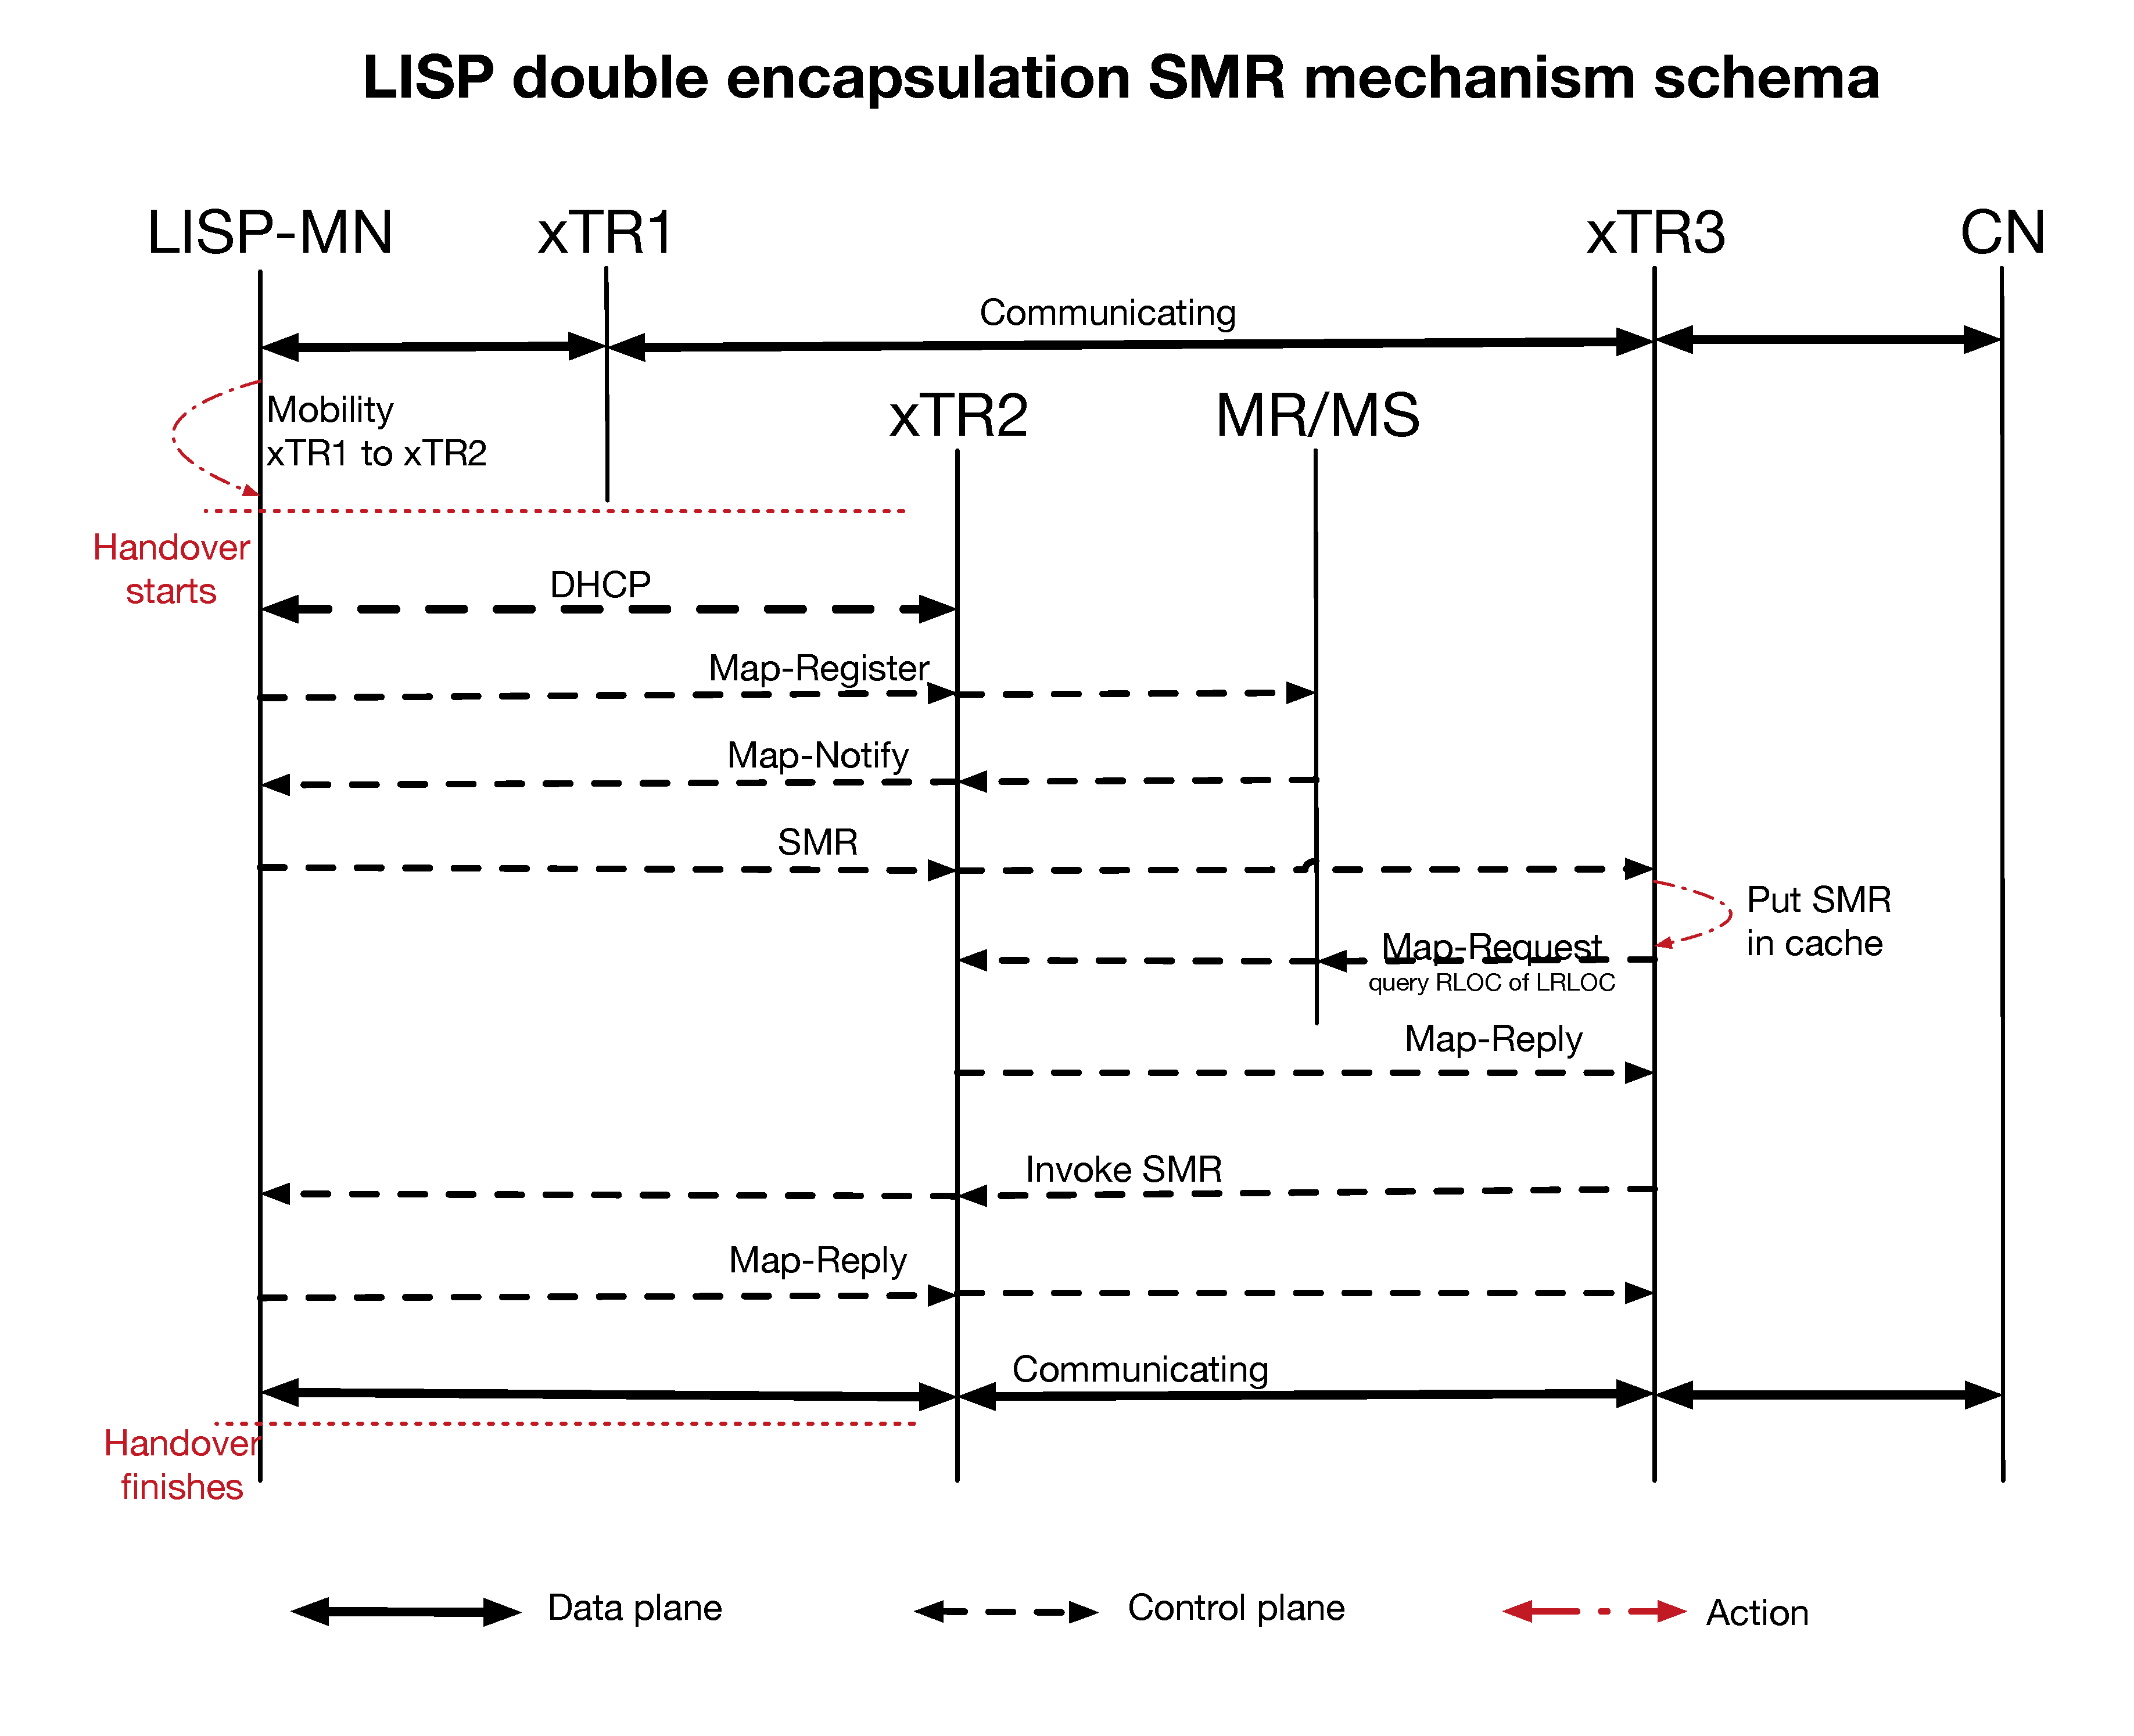
\includegraphics[width=0.8\textwidth]{Pics/Mobility_double_encap_schema_SMR_improving_simplify}
%	\caption{Schema for LISP-MN in LISP-Site mobility}
%	\label{Mobility_double_encap_schema_SMR_improving_simplify}
%\end{figure}
%%-< END FIGURE >--------------------------------------------------------------------
%If we do not consider the security issues, the handover schema can be simplified as shown in Fig.~\ref{Mobility_double_encap_schema_SMR_improving_simplify}.
%\begin{eqnarray}
%	D_{overall} &=& D_{DHCP} + D_{Register} + D_{Notify} + D_{SMR} + D_{Request} + D_{Reply} + D_{Request_{SMR}} + D_{Reply} \nonumber \\
%	&=& D_{DHCP} + 2T_{LISPMN-MDS} + D_{Resolve} + 3T_{LISPMN-xTR_3} \nonumber \\
%	&=& D_{DHCP} + 2* (3*2ms) + 200ms + 3*(3*2ms) \nonumber \\
%	&=& D_{DHCP} + 230 ms
%\end{eqnarray}
%where $D$ is the delay, $BI$ is Beacon Interval, subscriptions $Wi-Fi$, $DHCP$ and $SMR$ respectively refers to Wi-Fi association, DHCP procedure and LISP SMR. (Min value of handover delay = 1.300349, where packet sending interval = 0.02 s) 
%
%After several executions of simulation program, we observe that the overall handover delay changes by the various beacon intervals, in particular the Wi-Fi association delay depends on the different beacon intervals, whereas LISP SMR procedure always cost around $3s$. To get the lower bound of overall handover delay, we can ignore the Wi-Fi association delay when the beacon interval is $500ms$, and the latency due to DHCP procedure is always $1s$. Thus, adopting LISP-MN to conduct the host-based mobility takes at least $4s$. Compared to current most stable solution for host-based IP mobility management MIPv6, which latency including L2 and L3 in a real Wi-Fi testbed is around $3.68s$~\cite{vassiliou2010analysis}, LISP-MN has a higher delay caused by the double encapsulation mechanism introduced by LISP-MN behind LISP-Site. 
%
%During handover, CN can successfully receive packets from LISP-MN right after DHCP procedure being accomplished, but LISP-MN cannot receive the packets from CN until LISP SMR procedure is also finished. Thus, during DHCP procedure, all bi-directional transmitted packets are lost. To improve the performance, \cite{tang2017lisp} proposes a network-level LISP-MN solution, but has not validated their proposals neither in simulation nor in testbed. Our ns-3 implementation can be used to realize them.

Since both the MN and the border routers support LISP, the advantages of this scenario, i.e., LISP-MN in the LISP-Site, are: 
\begin{inparaenum}[1)]
	\item it can help to reduce the BGP routing table size;
	\item it is able to achieve handover through different subnets.
\end{inparaenum}
However, same to the shortcomings for the first scenario, each LISP-MN needs a permanent IP address as its EID, which increases the burden of IPv4 address allocation. Each permanent EID and its LRLOC needs register to the mapping system, which also increases the size of LISP mapping table. Besides, the numerical analysis indicates that the overall handover delay is much longer than the other two scenarios due to its double encapsulation.

Depend on our designed topology, all the aforementioned analyzed results are presented in Fig.~\ref{handover_delay_overhead_bar}. The left hand figure is the numerical overall handover delay related to LISP and right hand figure is about the handover overhead.
\begin{figure}[!t]
	\begin{minipage}[c]{.5\linewidth}
		\begin{center}
			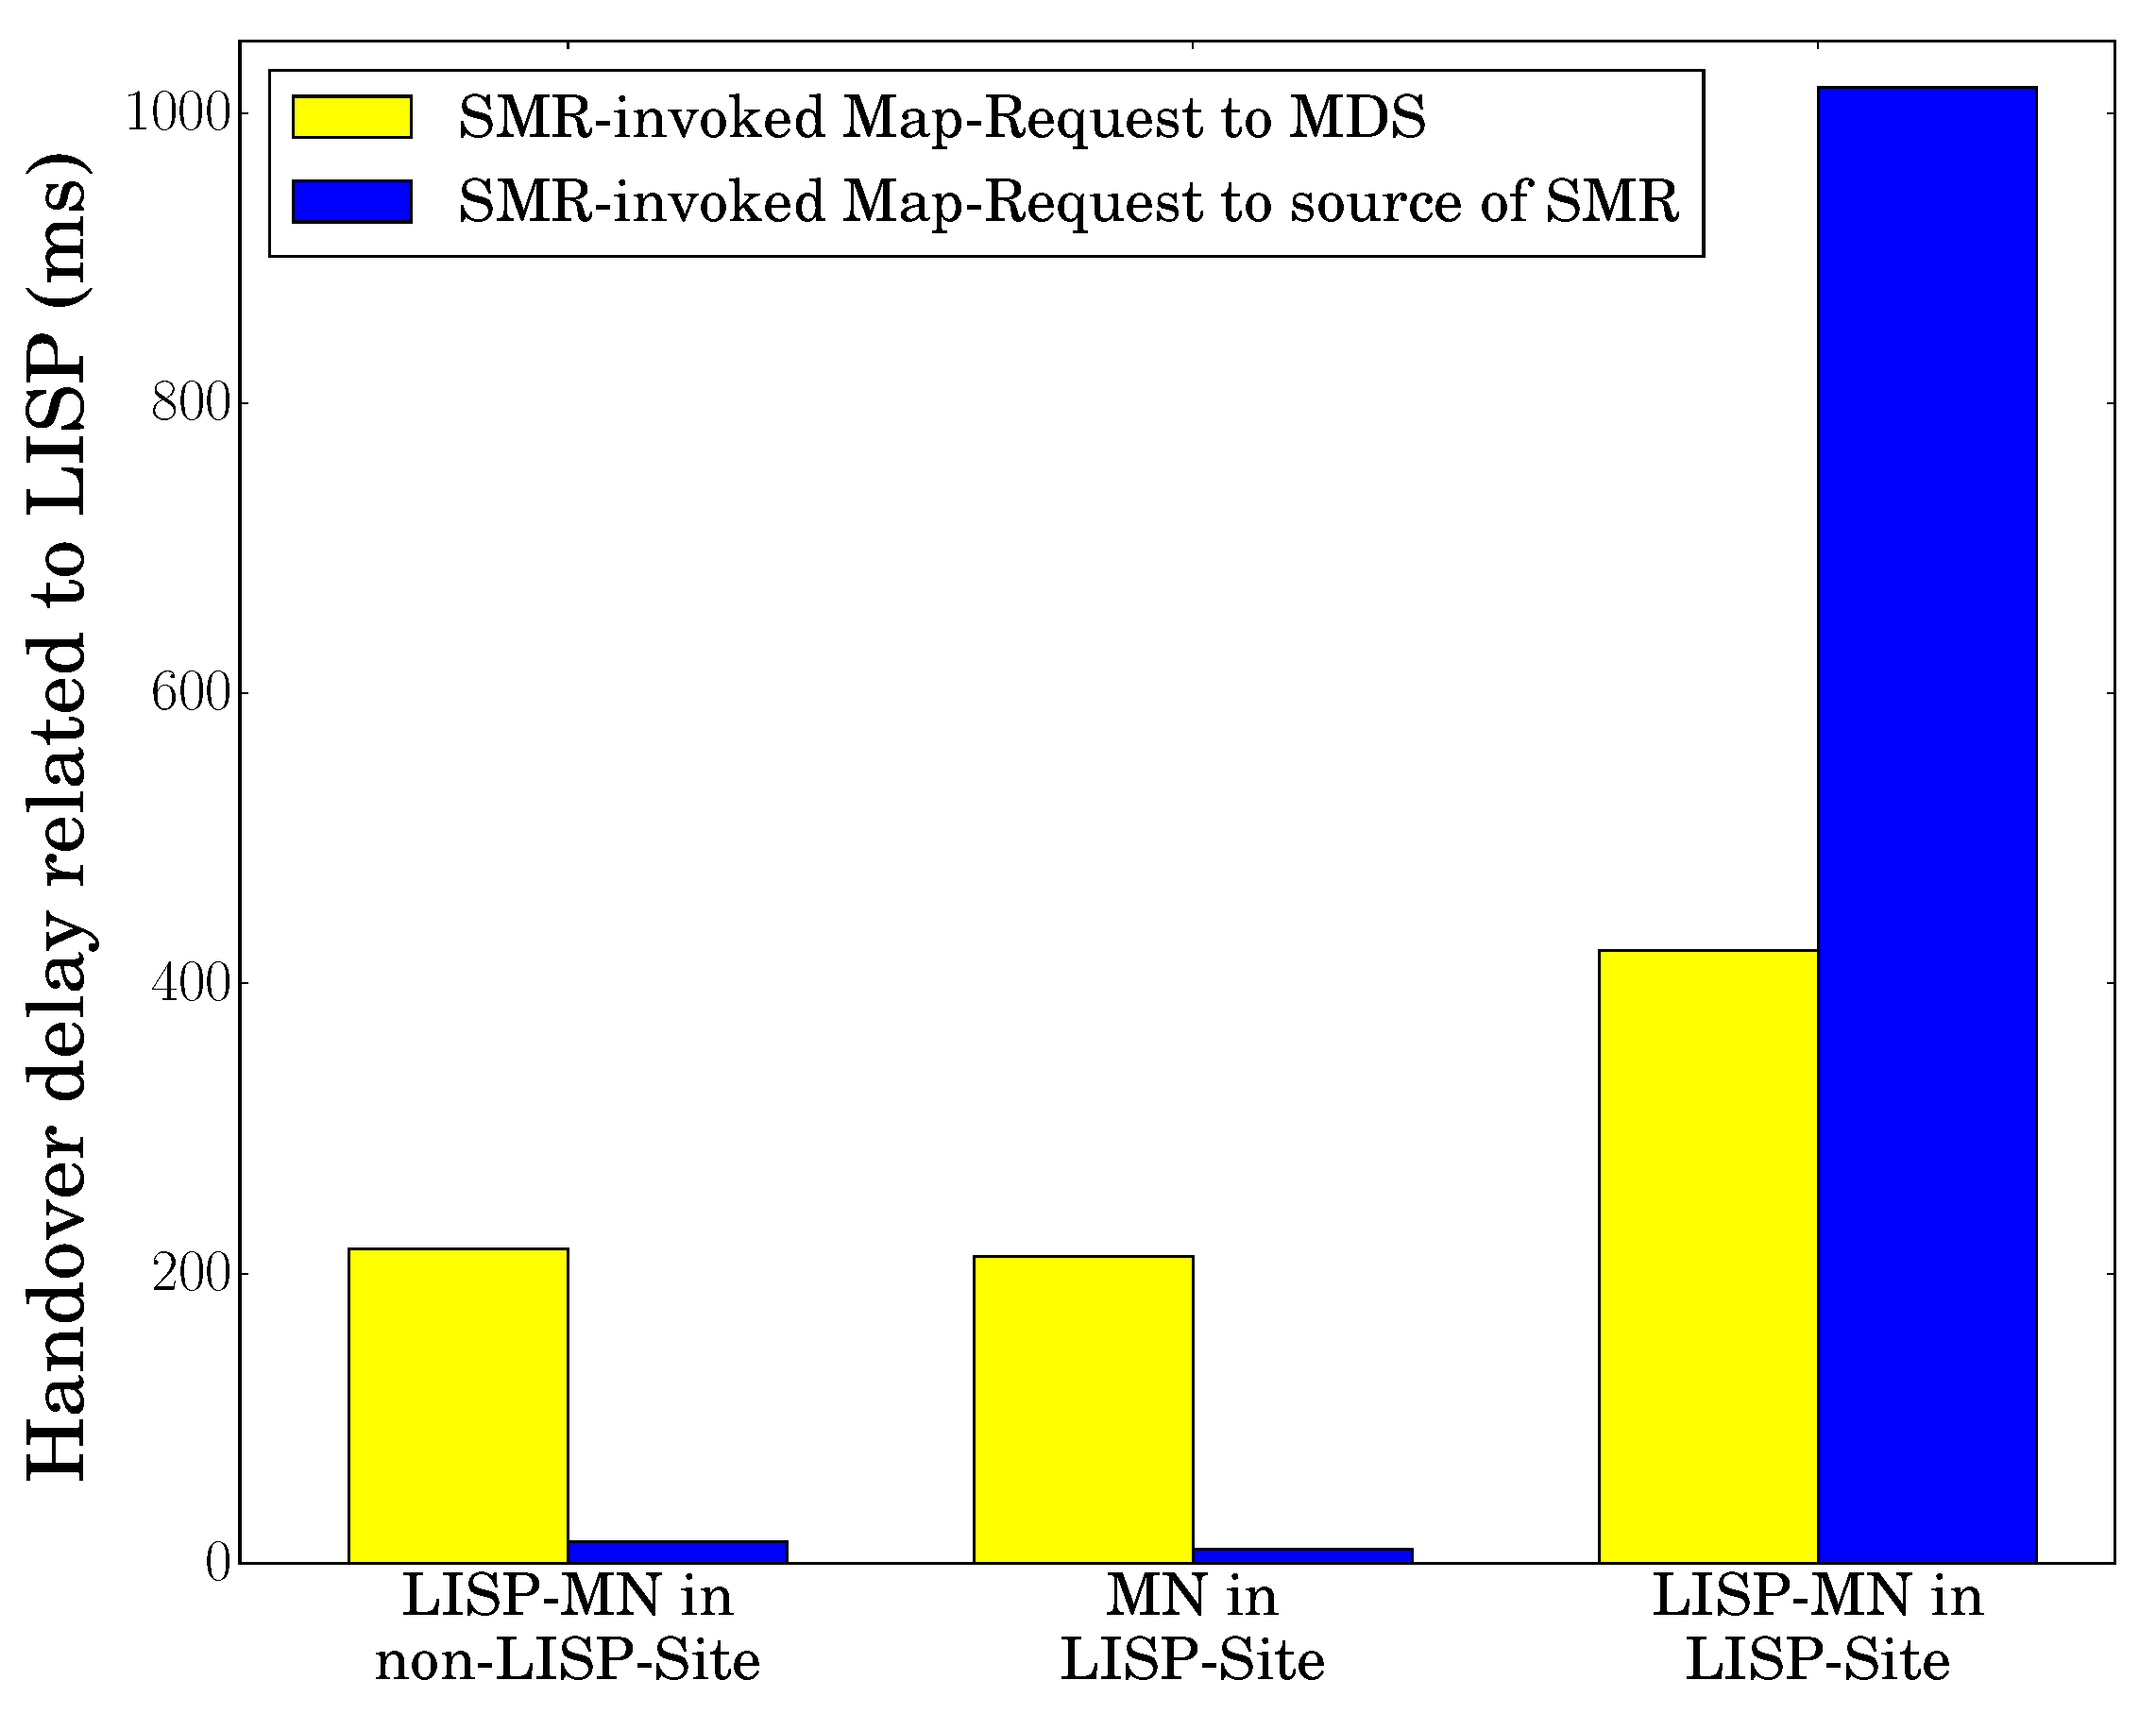
\includegraphics[width=\linewidth]{Pics/LISP_handover_delay_Bar.eps}
		\end{center}
	\end{minipage}
	\begin{minipage}[c]{.5\linewidth}
		\begin{center}
			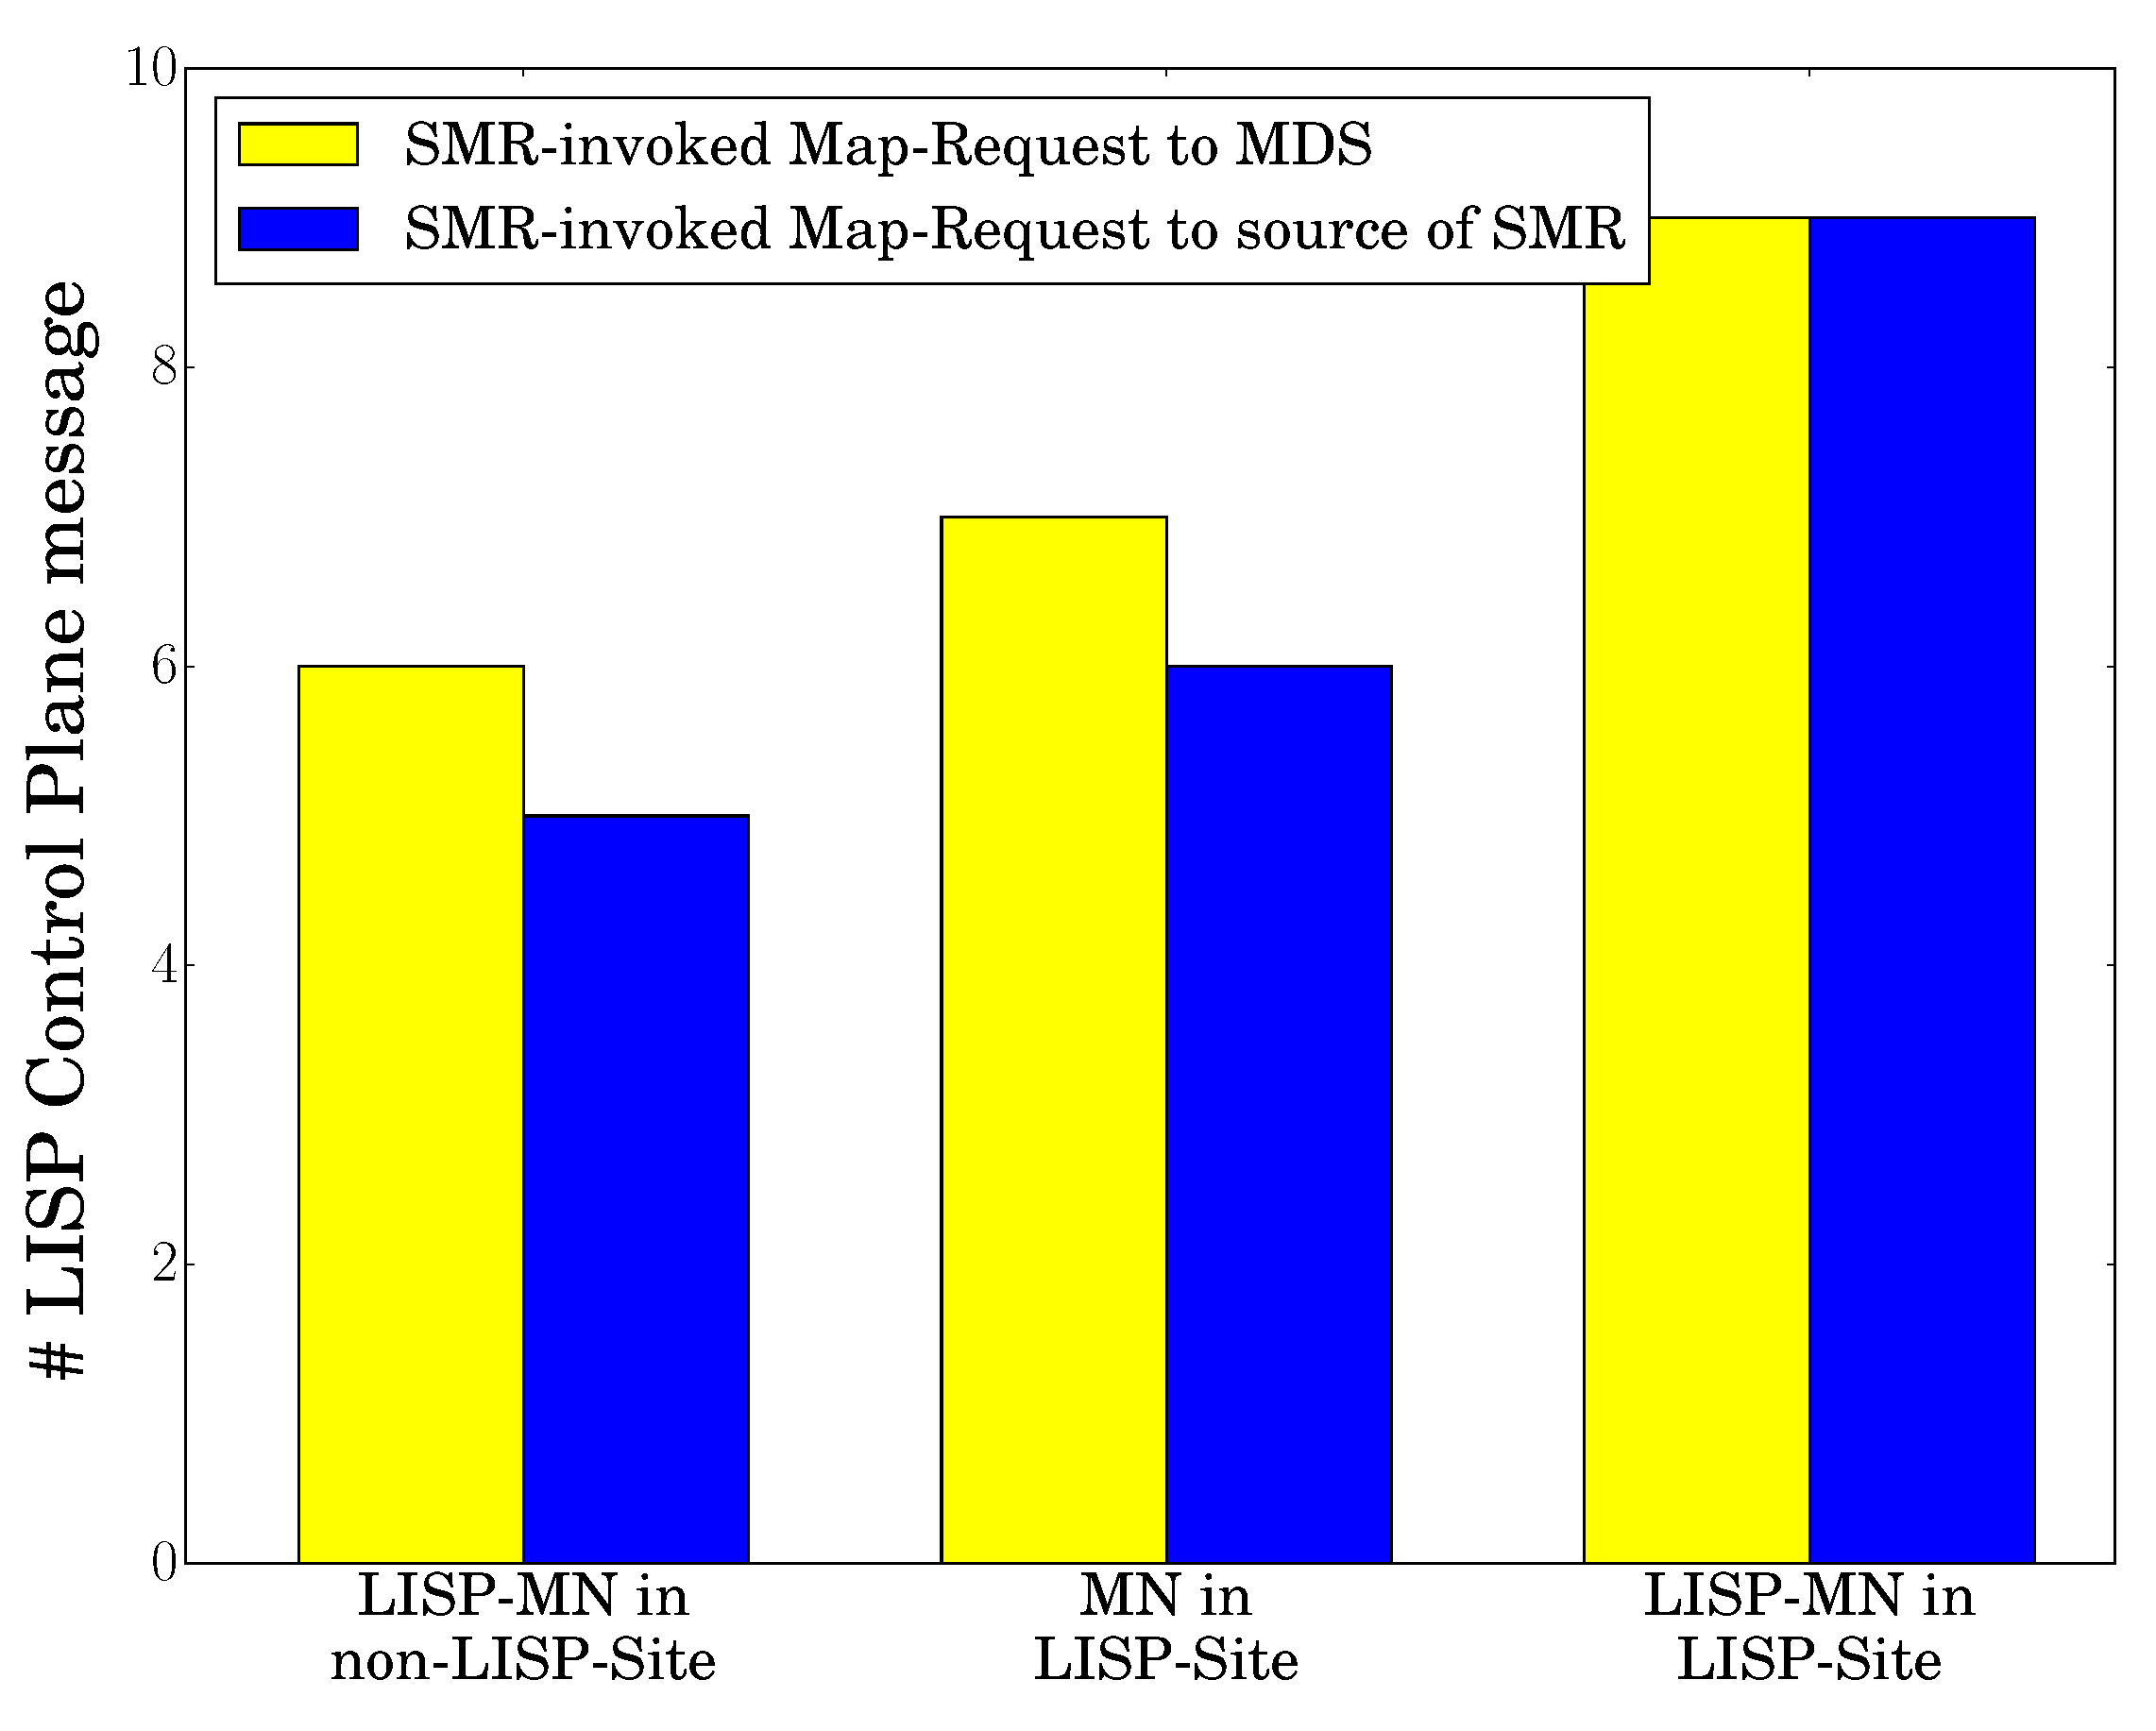
\includegraphics[width=\linewidth]{Pics/LISP_handover_overhead_Bar}
		\end{center}
	\end{minipage}
	\caption{The handover delay related to LISP (left) and the handover overhead (right) grouped by three LISP mobility scenarios.}
	\label{handover_delay_overhead_bar}
\end{figure}

%%-< SECTION >--------------------------------------------------------------------
%\section{Evaluations}
%\label{sec:ns3_evaluation}
% It runs an \emph{echo} application which sends packets to an \emph{echo} server on a remote stationary node CN situated in the LISP-Site of $xTR_3$.
% Every link between two network entities in this simulation architecture is set to $2 ms$. According to the experimental results in~\cite{coras2014performance}, we set the resolving time in the mapping system as $200 ms$.
%%-< FIGURE >--------------------------------------------------------------------
%\begin{figure}[!t]
%	\centering
%	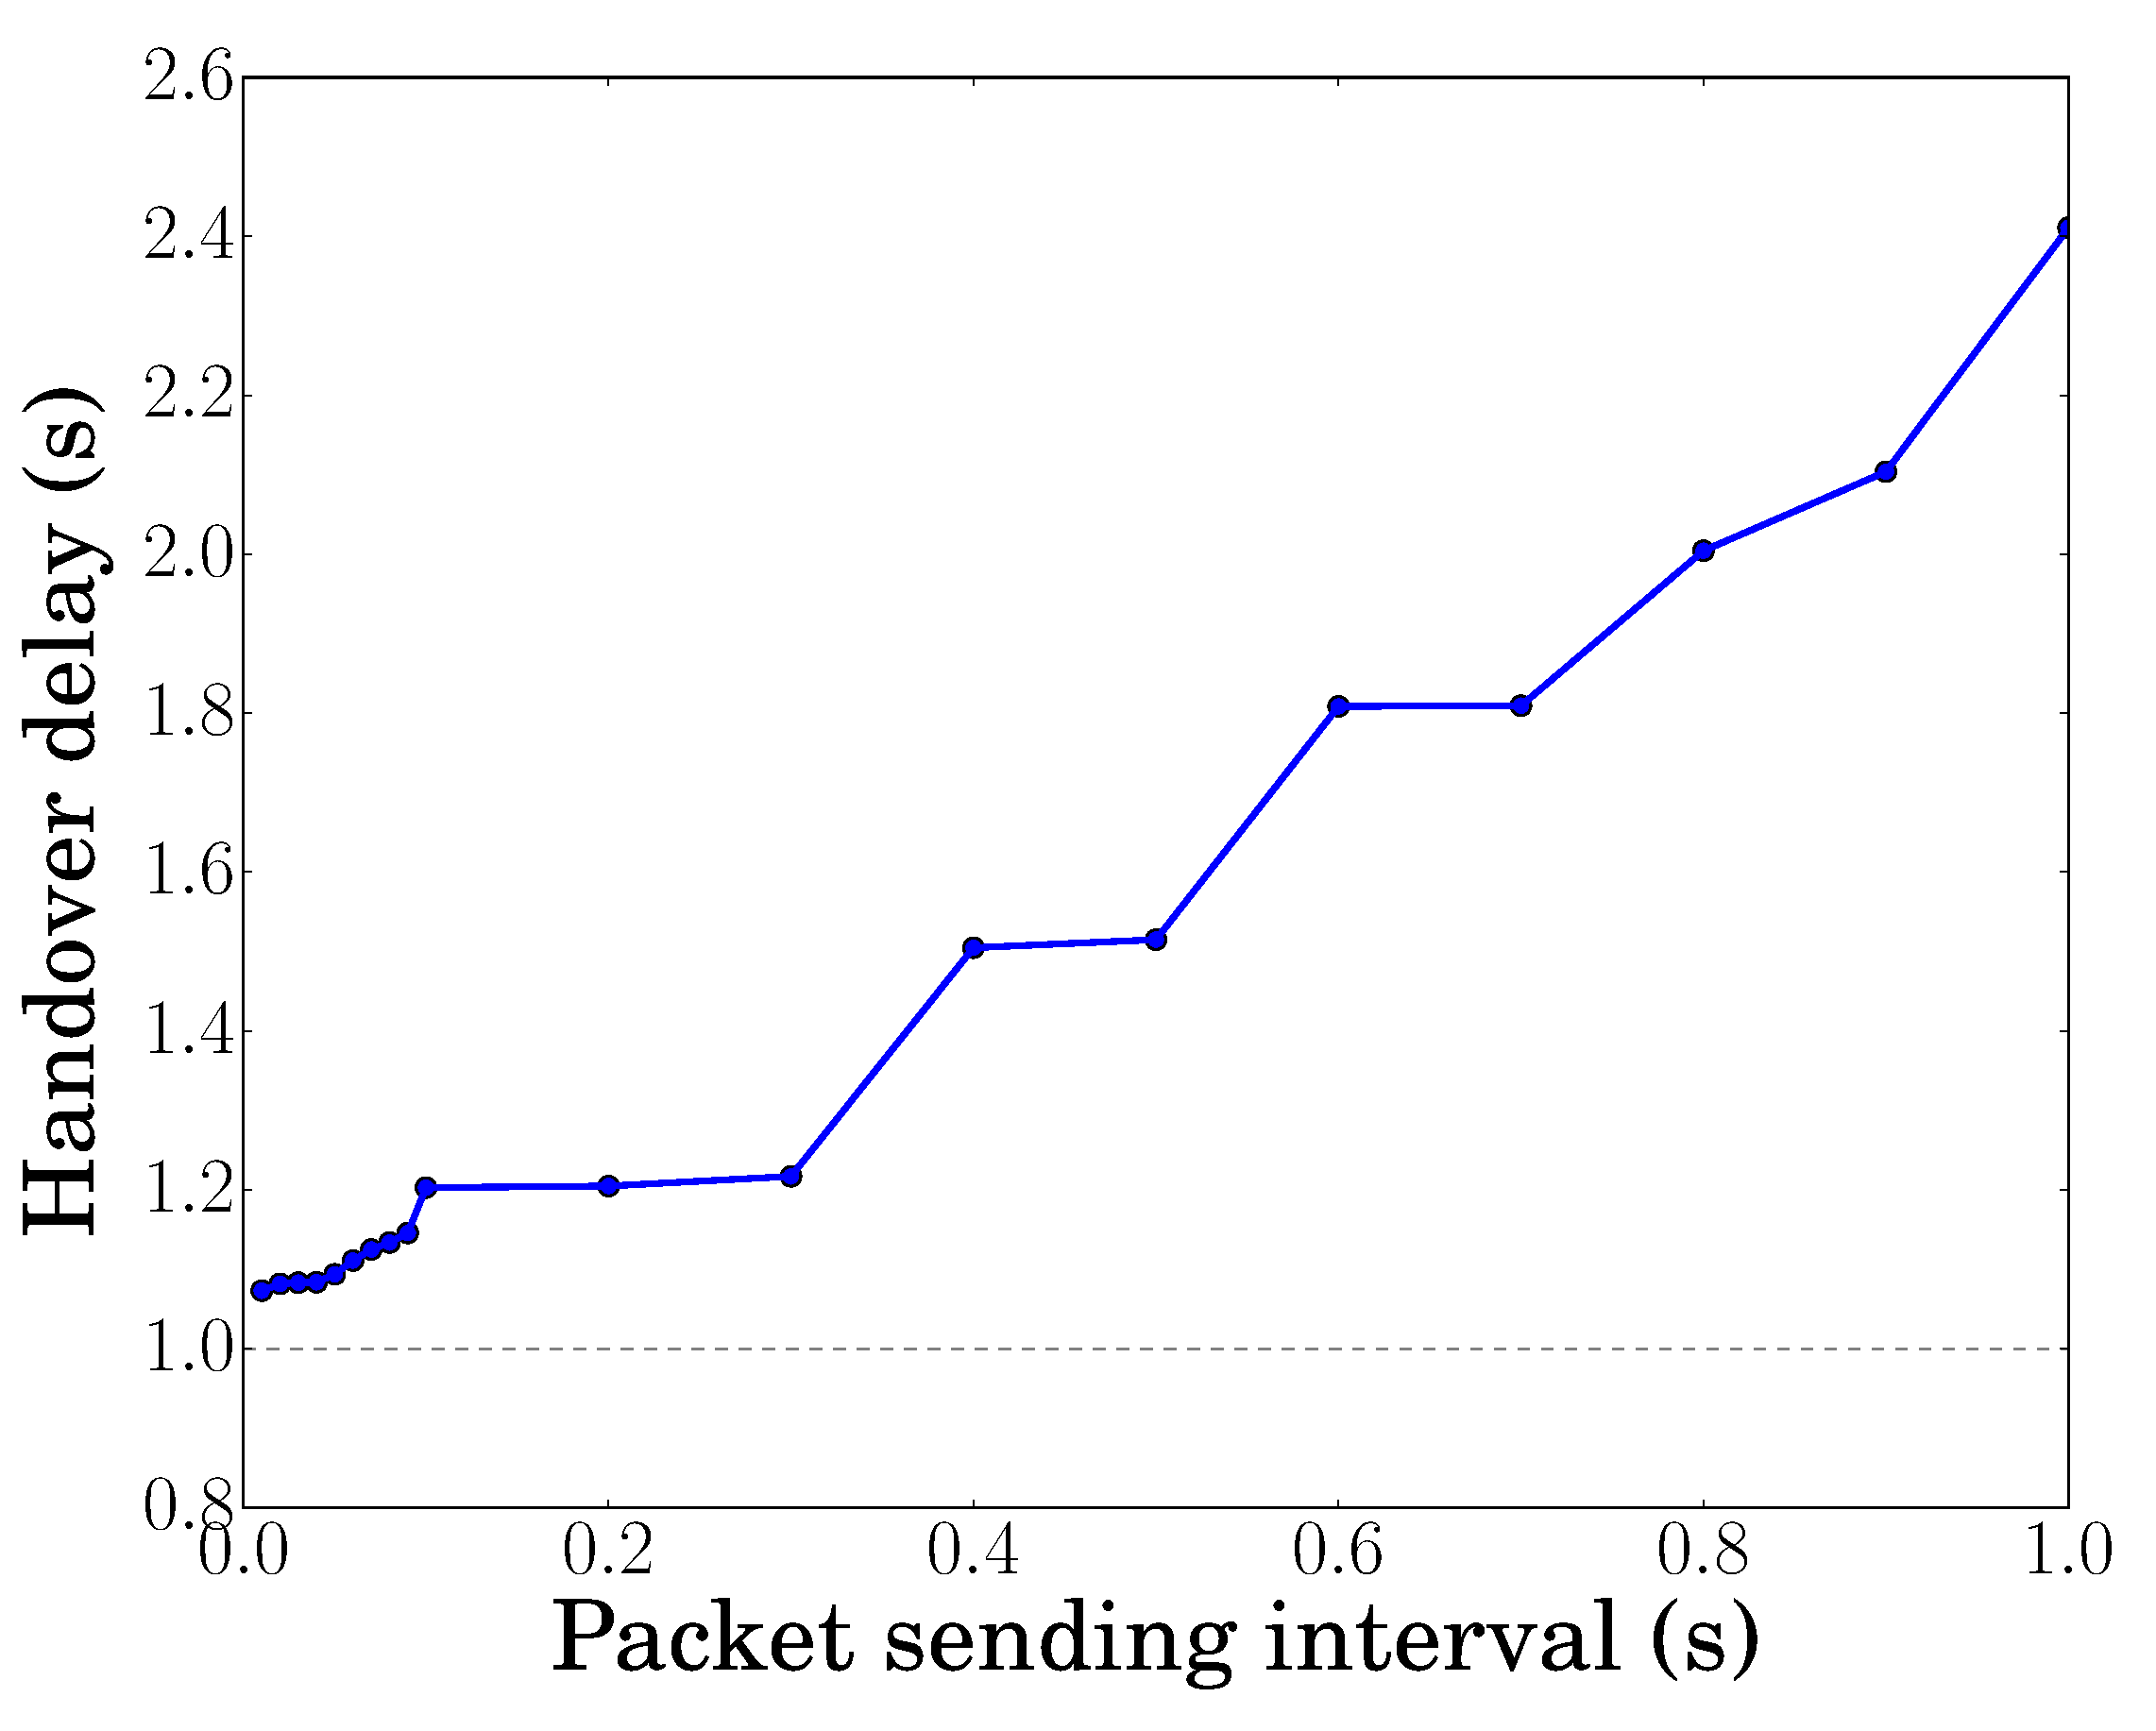
\includegraphics[width=0.7\textwidth]{Pics/LISP_mobility_LISPMN_PacketInterval}
%	\caption{Impact of packet sending interval on handover delay}
%	\label{LISP_mobility_LISPMN_PacketInterval}
%\end{figure}
%%-< END FIGURE >--------------------------------------------------------------------
%
%%-< FIGURE >--------------------------------------------------------------------
%\begin{figure}[!t]
%	\centering
%	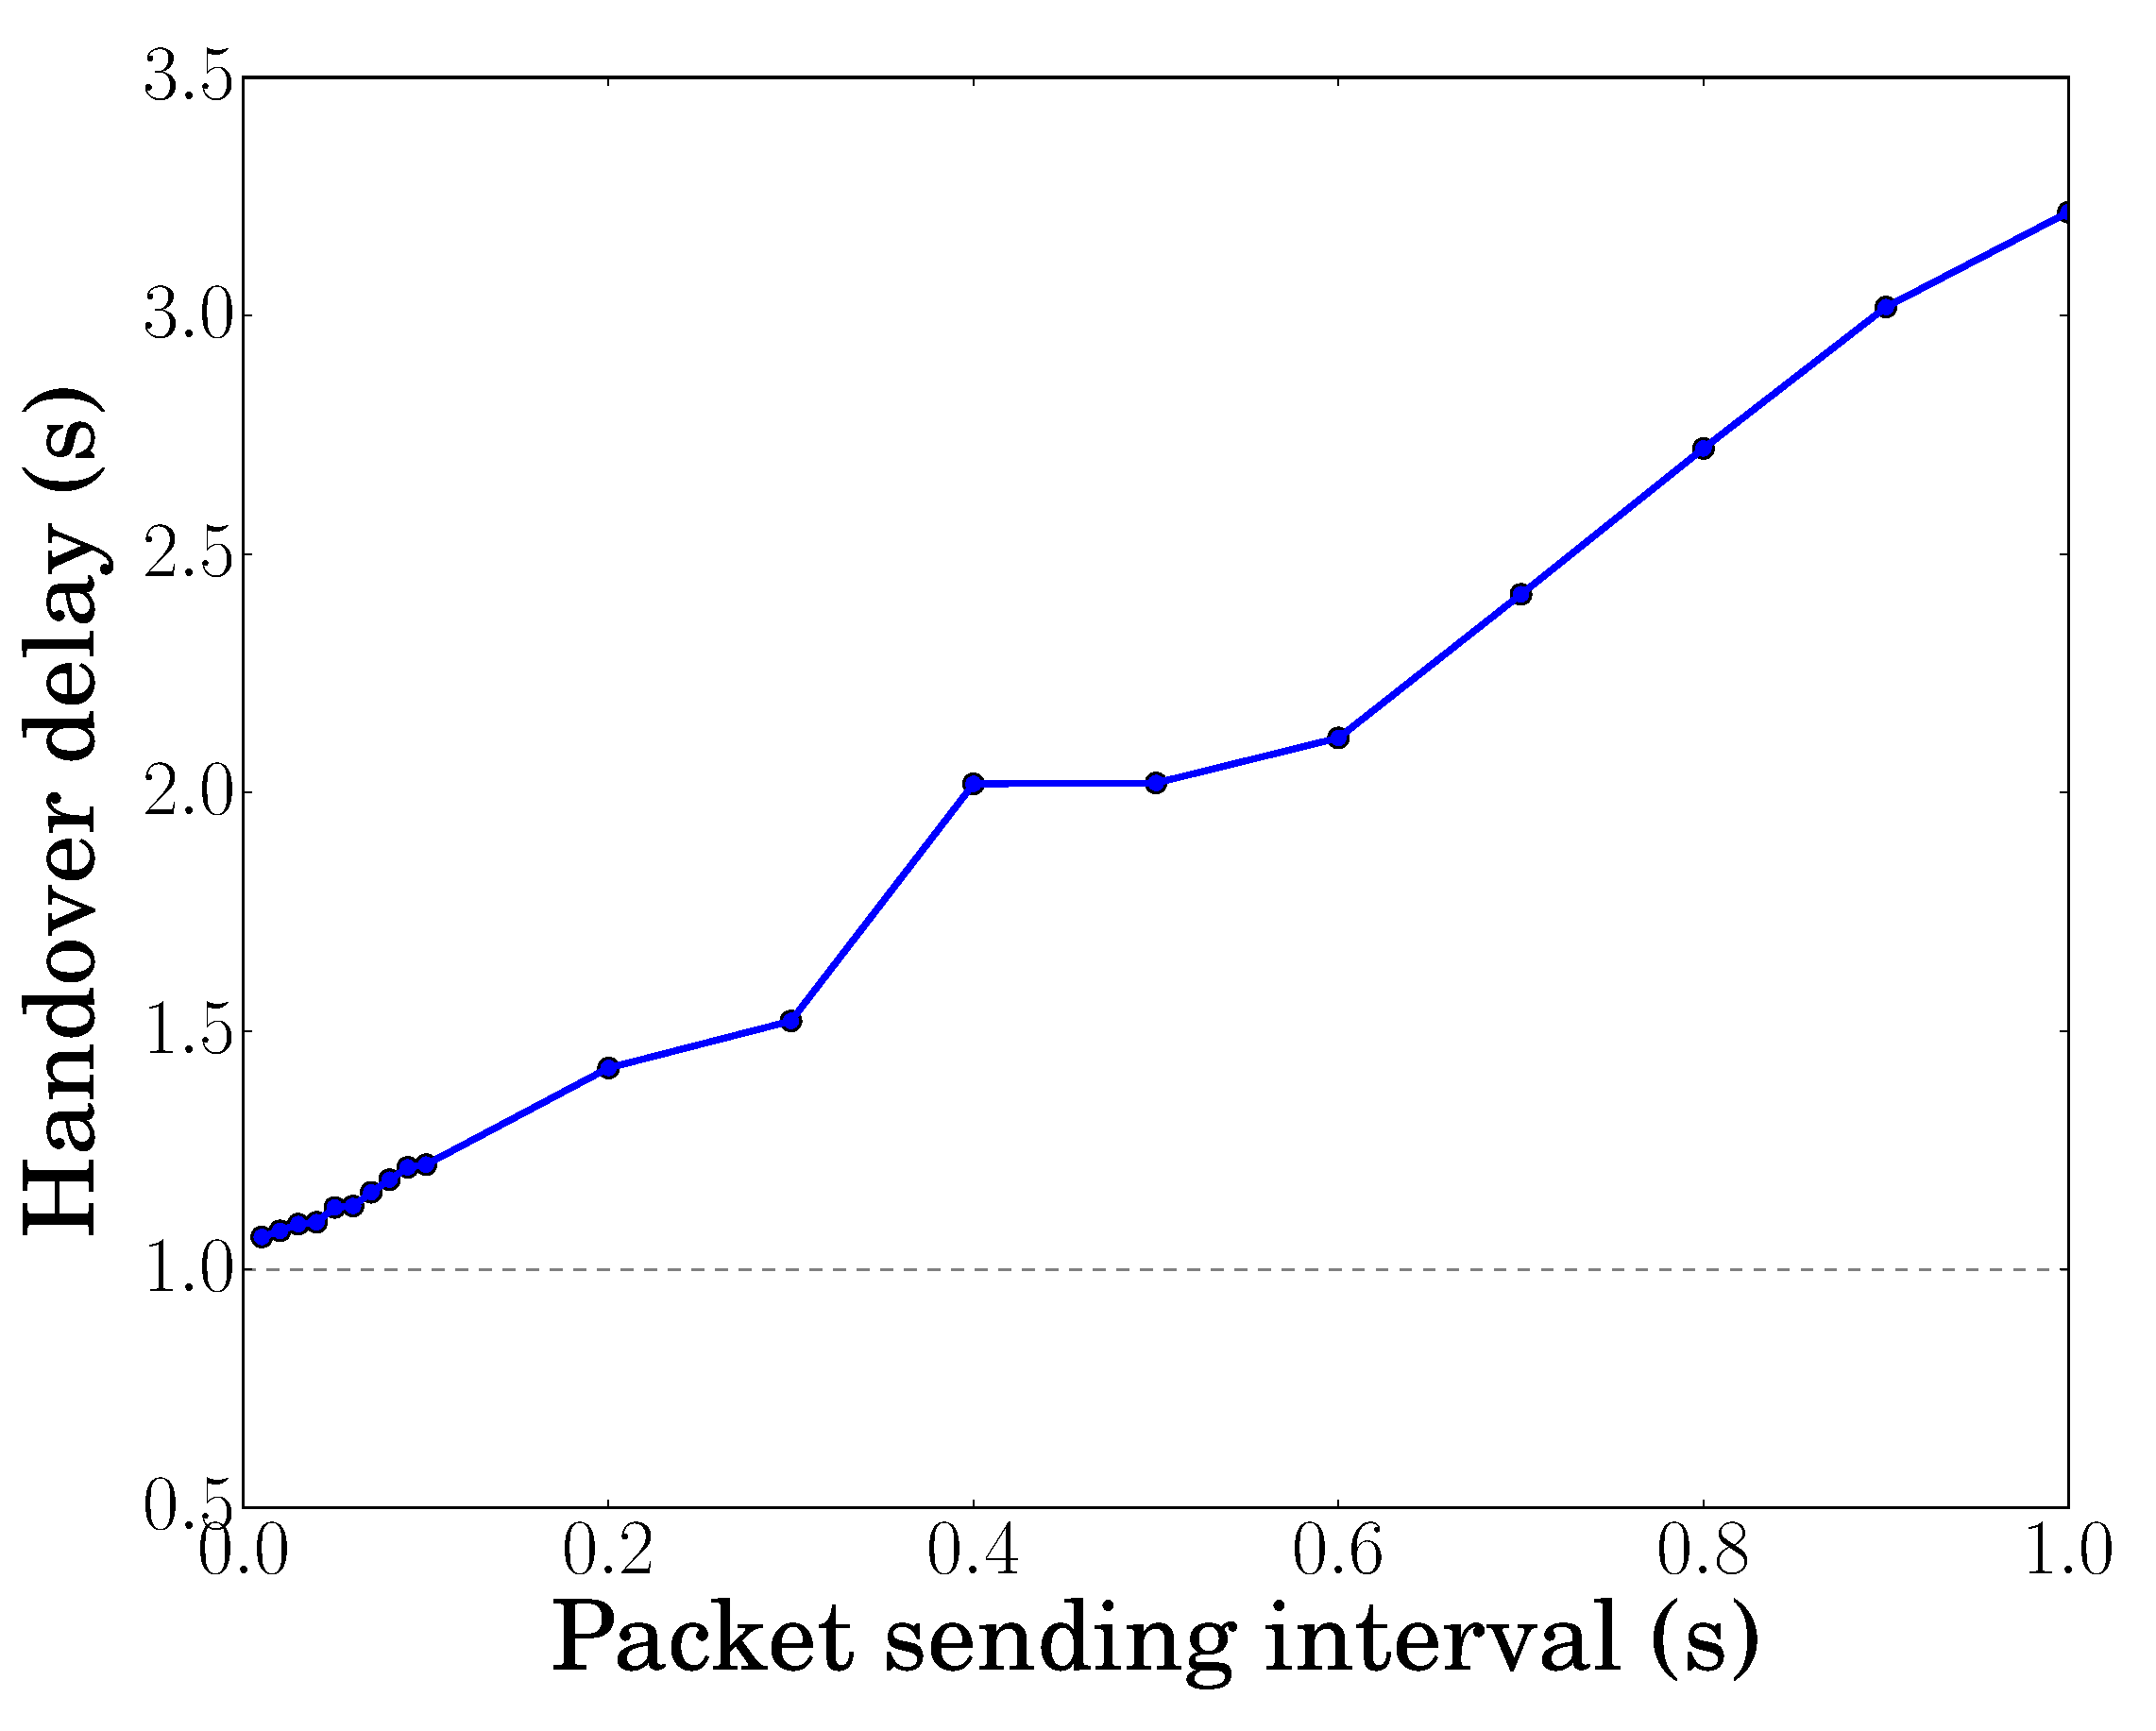
\includegraphics[width=0.7\textwidth]{Pics/LISP_mobility_xTR_PacketInterval}
%	\caption{Impact of packet sending interval on handover delay}
%	\label{LISP_mobility_xTR_PacketInterval}
%\end{figure}
%%-< END FIGURE >--------------------------------------------------------------------
%
%%-< FIGURE >--------------------------------------------------------------------
%\begin{figure}[!t]
%	\centering
%	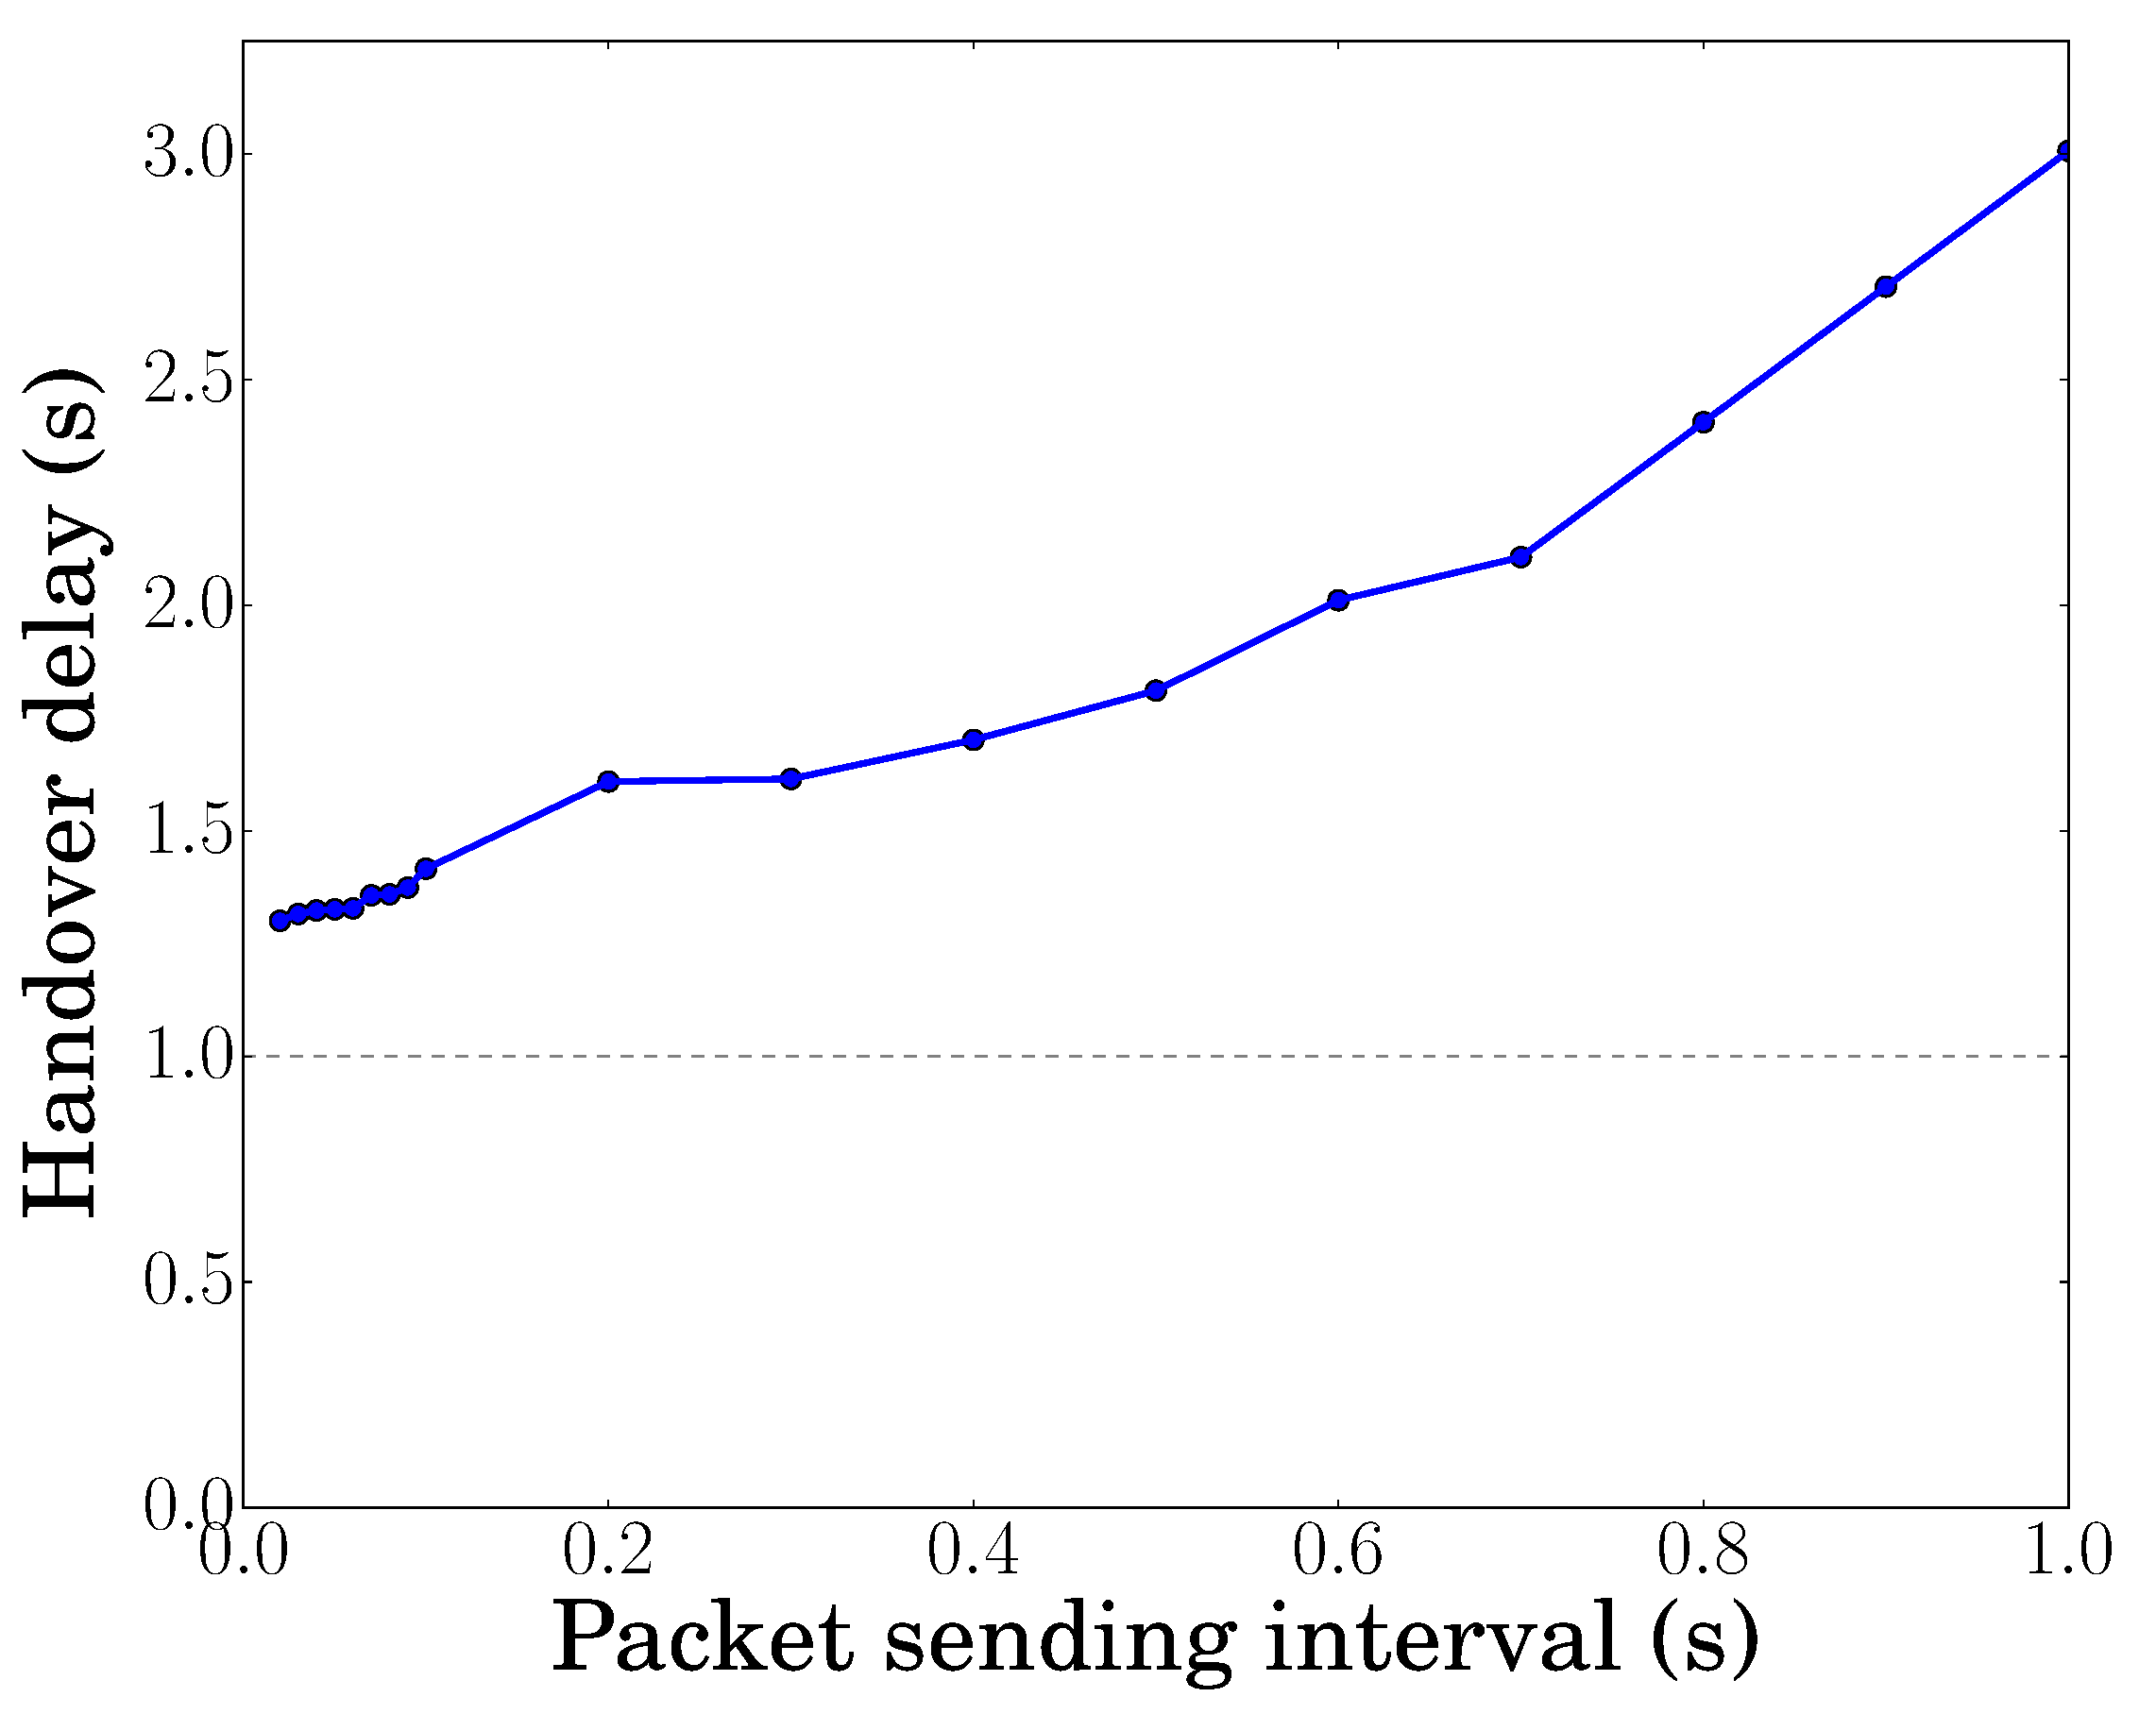
\includegraphics[width=0.7\textwidth]{Pics/LISP_mobility_double_encap_PacketInterval}
%	\caption{Impact of packet sending interval on handover delay}
%	\label{LISP_mobility_double_encap_PacketInterval}
%\end{figure}
%%-< END FIGURE >--------------------------------------------------------------------

%-< SECTION >--------------------------------------------------------------------

\section{Summary}
\label{sec:ns3_conclusion}
%\begin{itemize}
%    \item The validation of the implemented simulator
%    \item LISP-MN handover analysis
%    \item The potential of the implemented simulator
%\end{itemize}
% As a promising technology for the future Internet architecture, LISP attracts more and more attention. 
There exist some LISP simulation implementations, but they are proprietary or they do not support the extension of LISP mobility. Further, although measurements on LISP-testbeds can provide real time performance, due to the complicated topological structure, it is somewhat like a black box test, which hinders us to find the exact explanation for some results. This highlights the importance to have an open source simulator for LISP in particular to support LISP mobility functionality. In this chapter, based on an implementation of basic LISP on ns-3.24, we adapt it to ns-3.27 first (the latest version at the moment of writing). To facilitate the researchers to deeply track the exchange of LISP packets, we encode in LISP Data Plane packets so that the Wireshark can resolve them. Finally we implement the LISP mobility extensions on it. As there are three methods to support mobility in LISP: host-based (i.e. LISP-MN), network-based (i.e., xTR), both host-based and network-based (i.e., LISP-MN behinds xTR) mobility. We analyze the overall handover delay and the overhead of LISP Control Plane among them, compare the performance among them by listing their advantages and shortcomings. At the moment of writing, we are working on the simulation evaluation of the mobility scenarios. % The simulation results show that our implementation works well, and reveal the current LISP-MN proposal with a double encapsulation that has an high level delay during handover procedure. Our simulator can be a perfect choice to test the improvements of LISP-MN.


